% Options for packages loaded elsewhere
\PassOptionsToPackage{unicode}{hyperref}
\PassOptionsToPackage{hyphens}{url}
%
\documentclass[
]{article}
\usepackage{amsmath,amssymb}
\usepackage{iftex}
\ifPDFTeX
  \usepackage[T1]{fontenc}
  \usepackage[utf8]{inputenc}
  \usepackage{textcomp} % provide euro and other symbols
\else % if luatex or xetex
  \usepackage{unicode-math} % this also loads fontspec
  \defaultfontfeatures{Scale=MatchLowercase}
  \defaultfontfeatures[\rmfamily]{Ligatures=TeX,Scale=1}
\fi
\usepackage{lmodern}
\ifPDFTeX\else
  % xetex/luatex font selection
\fi
% Use upquote if available, for straight quotes in verbatim environments
\IfFileExists{upquote.sty}{\usepackage{upquote}}{}
\IfFileExists{microtype.sty}{% use microtype if available
  \usepackage[]{microtype}
  \UseMicrotypeSet[protrusion]{basicmath} % disable protrusion for tt fonts
}{}
\makeatletter
\@ifundefined{KOMAClassName}{% if non-KOMA class
  \IfFileExists{parskip.sty}{%
    \usepackage{parskip}
  }{% else
    \setlength{\parindent}{0pt}
    \setlength{\parskip}{6pt plus 2pt minus 1pt}}
}{% if KOMA class
  \KOMAoptions{parskip=half}}
\makeatother
\usepackage{xcolor}
\usepackage[margin=1in]{geometry}
\usepackage{longtable,booktabs,array}
\usepackage{calc} % for calculating minipage widths
% Correct order of tables after \paragraph or \subparagraph
\usepackage{etoolbox}
\makeatletter
\patchcmd\longtable{\par}{\if@noskipsec\mbox{}\fi\par}{}{}
\makeatother
% Allow footnotes in longtable head/foot
\IfFileExists{footnotehyper.sty}{\usepackage{footnotehyper}}{\usepackage{footnote}}
\makesavenoteenv{longtable}
\usepackage{graphicx}
\makeatletter
\def\maxwidth{\ifdim\Gin@nat@width>\linewidth\linewidth\else\Gin@nat@width\fi}
\def\maxheight{\ifdim\Gin@nat@height>\textheight\textheight\else\Gin@nat@height\fi}
\makeatother
% Scale images if necessary, so that they will not overflow the page
% margins by default, and it is still possible to overwrite the defaults
% using explicit options in \includegraphics[width, height, ...]{}
\setkeys{Gin}{width=\maxwidth,height=\maxheight,keepaspectratio}
% Set default figure placement to htbp
\makeatletter
\def\fps@figure{htbp}
\makeatother
\setlength{\emergencystretch}{3em} % prevent overfull lines
\providecommand{\tightlist}{%
  \setlength{\itemsep}{0pt}\setlength{\parskip}{0pt}}
\setcounter{secnumdepth}{5}
% definitions for citeproc citations
\NewDocumentCommand\citeproctext{}{}
\NewDocumentCommand\citeproc{mm}{%
  \begingroup\def\citeproctext{#2}\cite{#1}\endgroup}
\makeatletter
 % allow citations to break across lines
 \let\@cite@ofmt\@firstofone
 % avoid brackets around text for \cite:
 \def\@biblabel#1{}
 \def\@cite#1#2{{#1\if@tempswa , #2\fi}}
\makeatother
\newlength{\cslhangindent}
\setlength{\cslhangindent}{1.5em}
\newlength{\csllabelwidth}
\setlength{\csllabelwidth}{3em}
\newenvironment{CSLReferences}[2] % #1 hanging-indent, #2 entry-spacing
 {\begin{list}{}{%
  \setlength{\itemindent}{0pt}
  \setlength{\leftmargin}{0pt}
  \setlength{\parsep}{0pt}
  % turn on hanging indent if param 1 is 1
  \ifodd #1
   \setlength{\leftmargin}{\cslhangindent}
   \setlength{\itemindent}{-1\cslhangindent}
  \fi
  % set entry spacing
  \setlength{\itemsep}{#2\baselineskip}}}
 {\end{list}}
\usepackage{calc}
\newcommand{\CSLBlock}[1]{\hfill\break\parbox[t]{\linewidth}{\strut\ignorespaces#1\strut}}
\newcommand{\CSLLeftMargin}[1]{\parbox[t]{\csllabelwidth}{\strut#1\strut}}
\newcommand{\CSLRightInline}[1]{\parbox[t]{\linewidth - \csllabelwidth}{\strut#1\strut}}
\newcommand{\CSLIndent}[1]{\hspace{\cslhangindent}#1}
\usepackage{setspace}\linespread{1.25}
\usepackage[fontsize=12pt]{scrextend}
\usepackage[left]{lineno}
\usepackage[labelformat=empty]{caption}
\usepackage{longtable}
\usepackage{booktabs}
\ifLuaTeX
  \usepackage{selnolig}  % disable illegal ligatures
\fi
\usepackage{bookmark}
\IfFileExists{xurl.sty}{\usepackage{xurl}}{} % add URL line breaks if available
\urlstyle{same}
\hypersetup{
  hidelinks,
  pdfcreator={LaTeX via pandoc}}

\author{}
\date{\vspace{-2.5em}}

\begin{document}

\textbf{N-Methyl-D-aspartate receptor hypofunction causes recurrent and
transient failures of perceptual inference}\\
\strut \\

\textbf{Authors}:

Veith Weilnhammer\(^{1,2, 3,ec}\), Marcus Rothkirch\(^{1, 4, ec}\),
Deniz Yilmaz\(^{1,5,6,7, ec}\), Merve Fritsch\(^{1}\), Lena Esther
Ptasczynski\(^{1,5}\), Katrin Reichenbach\(^{1}\), Lukas
Rödiger\(^{1}\), Philip Corlett\(^{8}\), Philipp Sterzer\(^{9}\)\\
\strut \\
\textbf{Affiliations}:

\(^{1}\) Department of Psychiatry, Charité-Universitätsmedizin Berlin,
corporate member of Freie Universität Berlin and Humboldt-Universität zu
Berlin, Germany\\
\(^{2}\) Berlin Institute of Health, Charité-Universitätsmedizin Berlin
and Max Delbrück Center, Germany\\
\(^{3}\) Helen Wills Neuroscience Institute, University of California
Berkeley, USA\\
\(^{4}\) Medical School Berlin, Hochschule für Gesundheit und Medizin,
Germany\\
\(^{5}\) Berlin School of Mind and Brain, Humboldt-Universität zu
Berlin, Germany\\
\(^{6}\) Max Planck School of Cognition, Leipzig, Germany\\
\(^{7}\) Department of Psychiatry and Psychotherapy, LMU University
Hospital, Munich, Germany\\
\(^{8}\) Department of Psychiatry, Yale University School of Medicine,
New Haven, USA\\
\(^{9}\) Department of Psychiatry (UPK), University of Basel,
Switzerland\\
\strut \\
\textbf{Contributions}:

\(^{ec}\) Equal contribution\\
\strut \\
\textbf{Corresponding Author}:

Veith Weilnhammer, Helen Wills Neuroscience Institute, University of
California Berkeley, USA, email:
\href{mailto:veith.weilnhammer@gmail.com}{\nolinkurl{veith.weilnhammer@gmail.com}}\\

\textbf{Running Title}: Failures of inference under ketamine

\textbf{Keywords}: schizophrenia, psychosis, ketamine, predictive
processing, bistable perception, modes of inference

\newpage

\linenumbers

\section{Abstract}\label{abstract}

Perception integrates external sensory signals with internal predictions
that reflect prior knowledge about the world. Previous research suggests
that this integration is governed by slow alternations between an
external mode, driven by sensory signals, and an internal mode, shaped
by prior knowledge. Using a double-blind, placebo-controlled, cross-over
experiment in healthy human participants, we investigated the effects of
the N-Methyl-D-aspartate receptor (NMDAR) antagonist S-ketamine on the
balance between external and internal modes. We found that S-ketamine
causes a shift of perception toward the external mode. A case-control
study revealed that individuals with paranoid Scz, a disorder repeatedly
associated with NMDAR hypofunction, spend more time in the external
mode. This NMDAR-dependent increase in the external mode suggests that
the symptoms of schizophrenia are caused by recurring dissociations of
perception from prior knowledge about the world.

\section{Introduction}\label{introduction}

Imagine a dimly lit room at a crowded party, where unclear visual
signals, indistinct sounds, and complex social interactions allow for
multiple - and sometimes false - interpretations. In such ambiguity,
failures of perceptual inference, the ability to contextualize sensory
inputs with prior knowledge about the world, can lead to profound
departures from reality: Faces obscured in shadow may appear distorted,
random noise could be perceived as a whisper, and friendly smiles might
seem derogatory.

According to the canonical predictive processing
hypothesis\textsuperscript{1}, a disruption of perceptual inference is
likely to play a crucial role in schizophrenia (Scz), a severe mental
disorder characterized by psychotic symptoms such as delusions and
hallucinations\textsuperscript{1--3}. People with Scz may fail to apply
prior knowledge to the interpretation of ambiguous sensory signals,
causing erratic inferences that lead to hallucinatory experiences and
delusional beliefs\textsuperscript{1}. Yet despite considerable progress
in the computational understanding of psychosis, two key questions have
remained unanswered.

The first question concerns the neural mechanisms that cause perceptual
inference to fail in Scz. Formal predictive processing accounts of Scz
foreground the role of prediction errors in updating Bayesian beliefs
about the causes of sensory input\textsuperscript{4}. Most accounts
focus on a failure to predict or instantiate the precision afforded to
prediction errors at various levels of the cortical
hierarchy\textsuperscript{1--3}. Precision refers to the confidence
ascribed to prediction errors, and regulates how prior expectations are
updated in response to sensory information\textsuperscript{4}.
Mathematically, precision is equivalent to the (Kalman) gain or the
weighting of prediction errors in predictive processing models of
perceptual inference\textsuperscript{5}. Psychologically, the deployment
of sensory precision can be understood in terms of selective attention
(or sensory attenuation)\textsuperscript{6,7}. Physiologically,
precision corresponds to the postsynaptic gain or excitability of
neuronal populations that report prediction errors, commonly mediated by
N-Methyl-D-aspartate receptors\textsuperscript{8--11} (NMDARs).

Beyond predictive processing theory, several lines of evidence point to
NMDAR hypofunction as a key factor in the pathophysiology of
psychosis\textsuperscript{12}. NMDAR antibodies\textsuperscript{13} and
antagonists such as ketamine\textsuperscript{14} mimic the symptoms of
Scz, which is itself associated with a reduction of NMDAR density in the
prefrontal cortex\textsuperscript{15}. In addition to their role in
controlling the excitability of prediction error
neurons\textsuperscript{8--11} and their general function for
maintaining the cortical excitation-inhibition
balance\textsuperscript{16}, NMDARs play a critical role in cortical
feedback\textsuperscript{17}, support synaptic short-term
plasticity\textsuperscript{18}, and interact with neuromodulators such
as dopamine and serotonin via GABAergic
interneurons\textsuperscript{19}. While these NMDAR-dependent mechanisms
are likely critical for perceptual inference, it is yet to be determined
how NMDAR hypofunction may cause the symptoms of Scz.

The second unresolved question concerns the temporal dynamics of
psychotic experiences, which often unfold as short-lived events spanning
from seconds to minutes, especially at early stages of Scz. The
transient nature of psychotic experiences\textsuperscript{20--22}
challenges models that assume a constant disruption of perceptual
inference\textsuperscript{1--3}. A solution to this problem is suggested
by the recent observation that perceptual inference is subject to
spontaneous fluctuations over time\textsuperscript{23--25}. Such
fluctuations have been related to two opposing modes of inference, or
shifts in attentional sets, during which perception is driven
predominantly either by external inputs (external mode) or by internal
predictions that stem from recent experiences\textsuperscript{26}
(internal mode, Figure 1A). Although preliminary evidence indicates a
tendency toward the external mode in people with
Scz\textsuperscript{27}, the neural mechanisms of mode fluctuations and
their potential implications for computational models of Scz have
remained elusive.

The objective of the current study was therefore twofold: First, to test
whether NMDAR hypofunction causes changes in perceptual inference that
characterize Scz; and second, to explore the effect of NMDAR
hypofunction on ongoing fluctuations in perceptual inference that may
explain the transient nature of psychotic experiences. We addressed
these questions in a double-blind, placebo-controlled, cross-over
experiment with S-ketamine in healthy participants, and a case-control
study that compared patients with paranoid Scz to matched healthy
controls\textsuperscript{28}. Participants engaged in a task designed to
test how internal predictions derived from previous experiences modulate
the perception of sensory signals that varied in ambiguity. We found
that NMDAR antagonism and Scz were associated with a shift of perception
toward the external mode, a minute-long state of the brain during which
inference dissociates from prior knowledge. Our results suggest that
NMDAR hypofunction shifts the balance between external and internal
modes, and may thus contribute to the symptoms of Scz by causing
transient and recurring failures of perceptual inference.

\section{Materials and Methods}\label{materials-and-methods}

\subsection{S-ketamine vs.~placebo}\label{s-ketamine-vs.-placebo}

The S-ketamine experiment consisted in a total of three experimental
sessions. During the first session, we screened participants for
S-ketamine contraindications (arterial hypertension, prior psychiatric
or neurological diagnoses including substance use disorder, use of
psychoactive medication), and assessed psychosis proneness using the
40-item \emph{Peters Delusion Inventory} (PDI\textsuperscript{29}) and
the 32-item \emph{Cardiff Anomalous Perception Scale}
(CAPS\textsuperscript{30}). Moreover, we conducted three experimental
pre-test runs that tested the ability to process stereodisparity (run 1,
SAR = 1, cut-off: perceptual accuracy \textgreater{} 0.75), ensured the
experience of spontaneous switches during bistable perception (run 2,
SAR = 0, cut-off: perceptual stability \textless{} 0.96, corresponding
to phase durations \textless{} 40 sec), and familiarized participants
with the main experiment (run 3, see below for details).

In the subsequent two sessions, participants received a continuous
intravenous infusion of either S-ketamine at 0.1 mg/kg/h or a saline
placebo. Health screenings were repeated before each session to ensure
the participants remained eligible. At each day of testing, we checked
for alcohol intoxication using a breathalyzer and for recent illicit
substance use via a urine drug screen.

Our experimental protocol was double-blinded: The order of S-ketamine
and placebo administration was counter-balanced across participants,
with at least a two week interval between sessions. The participants, as
well as the experimenters tasked with collecting the behavioral and
psychometric data, were unaware of whether S-ketamine or placebo was
administered by an independent group of clinicians who excluded
undiagnosed psychotic illness using the \emph{Brief Psychiatric Rating
Scale} (BPRS\textsuperscript{31}), established the intravenous line,
started the infusion 15 min prior to the experiment, monitored the
participants for side effects (blood pressure, drowsiness, vasovagal
reactions, and psychotomimetic effects), and removed the intravenous
line at the end of the experiment, after which participants were
monitored for at least 30 min. Deblinding occurred after data collection
was complete.

\subsubsection{Sample characteristics}\label{sample-characteristics}

We screened a total of 87 right-handed individuals with (corrected-to-)
normal vision, who were naive to the purpose of the study and gave
written informed consent before participating. All experimental
procedures were approved by the ethics committee at Charité Berlin.

From the group of screened participants, 31 did not meet our pretest
criteria (6 due to perceptual accuracy \textless{} 0.75, 15 due to
perceptual stability \textgreater{} 0.96, 8 due to substance use, 1 due
to do a diagnosis of ADHD, and 1 due to medication with sertraline). Out
of the remaining 56 participants who were eligible for the S-ketamine
experiment, we aborted the main experiment in 1 participant due to high
blood pressure at baseline (RR \textgreater{} 140/80 mmHG), in 2
participants due to strong psychotomimetic effects (micropsia) or
dizziness under S-ketamine, and in 1 participant due to a vasovagal
syncope during intravenous insertion. 24 participants were not available
for the main experiment after successful pre-testing. We therefore
report the data from a total of 28 participants (mean age: 28.93 ± 1.35
years, 18 female) who met all inclusion criteria and completed all
experimental sessions.

\subsubsection{Experimental paradigm}\label{experimental-paradigm}

We presented the experiment using Psychtoolbox 3\textsuperscript{32}
running in Matlab R2021b (session 1: CRT-monitor at 85 Hz, 1280 x 1024
pixels, 60 cm viewing distance and 39.12 pixels per degree visual angle;
session 2 and 32: CRT-monitor at 85Hz, 1280 x 1024 pixels, 40 cm viewing
distance and 26.95 pixels per degree visual angle).

\textbf{Procedure}: Throughout the experiment, participants reported
their perception of a structure-from-motion (SFM) stimulus (Supplemental
Video S1). In this stimulus, random dots distributed on two intersecting
rings induce the perception of a spherical object (diameter: 15.86°,
rotational speed: 12 sec per rotation, rotations per block: 10,
individual dot size: 0.12°) that rotates around a vertical axis with the
front surface to the left or right\textsuperscript{33}. Stimuli were
presented in 120 sec blocks, separated by 10 sec fixation intervals.
Please note that we assessed participants' perception of the stimulus
based on a fixed response mapping. In our paradigm, perception and
reports are therefore inherently intertwined, with the participants'
reports serving as the sole indicators of their perceptual states.

Participants viewed the stimuli through a custom mirror stereoscope. In
the pretest experiment, we presented stimuli at complete disambiguation
(run 1, SAR = 1), full ambiguity (run 2, SAR = 0) and across five levels
ranging from full ambiguity to complete disambiguation across five
levels (run 3-5, \(SAR \in \{0, 0.1, 0.25, 0.5, 1\}\)). The
signal-to-ambiguity ratio (SAR), which was constant within blocks,
defines the fraction of stimulus dots that carried a disambiguating 3D
signal.

Participants were naive to the potential ambiguity in the visual
display, passively experienced the stimulus and reported changes in
their perception alongside their confidence via button-presses on a
standard USB keyboard (right middle-finger on k: rotation of the
front-surface to the right at high confidence; right index-finger on j:
rotation of the front-surface to the right at low confidence; left
middle-finger on s: rotation of the front-surface to the left at high
confidence; left index-finger on d: rotation of the front-surface to the
left at low confidence; thumb on space bar: unclear direction of
rotation). Unclear perceptual states occurred at a rate of 0.03 ± 0.01
and were excluded from further analyses.

The direction of rotation enforced by \(s_t\) (i.e., whether the
parametric 3D signal enforced leftward or rightward rotation of the
front surface) changed at a rate of 0.15 per overlap (i.e., on average
every 10 sec). Changes in \(s_t\) and the order of blocks, each
corresponding to one level of SAR, were pseudo-random.

In session 1 (pre-test), each run (runs 1 to 3) consisted of six blocks.
In session 2 and 3 (main experiment), each run (run 4 and 5) consisted
of 10 blocks. After every third block, the main experiment was paused to
allow for the monitoring of the participants' vital signs (blood
pressure and pulse rate) and dynamic changes in psychotomimetic
experiences. The latter was assessed using the 6 item
\emph{Clinician-Administered-Dissociative-States-Scale}
(CADSS\textsuperscript{34}) and three additional questions (Q1:
\emph{How awake do you feel?}, Q2: \emph{How intoxicated do you feel?},
Q3: \emph{How nervous do you feel?}) to which participants responded by
clicking on a continuous line that encoded responses from \emph{not at
all} to \emph{very much}. To measure global psychotomimetic effects of
S-ketamine vs.~placebo, participants completed the Questionnaire for the
\emph{Assessment of Altered States of Consciousness}
(5D-ASC\textsuperscript{35}) at the end of session 2 and 3. In addition,
we collected responses on a debriefing questionnaire, in which we asked
participants to describe whether they were able to accurately perceive
the two directions of rotation induced by the SFM stimulus, whether they
noticed any differences between blocks, whether they would guess that
they received S-ketamine or placebo, and whether they had experienced
any effects that they would attribute to a psychoactive substance.

\textbf{Stereodisparity thresholds:} At the beginning of the session 2
and 3, we conducted an independent stereo-acuity test to detect a
potential effect of S-ketamine on stereodisparity
thresholds\textsuperscript{28}. We presented 5000 dots (each at 0.15°
visual angle) within a square of 11° x 11° around a central fixation
cross (0.10°). We added a stereodisparity signal to all dots on a
Landolt C, i.e., a circle (1.37° radius, 2.06° width) with a 90° gap
located either at the left, top, right or bottom. Stimuli were presented
for 1 sec, after which participants reported the location of the gap by
pressing the up-, down-, left- or right-arrow key within a 2 sec
response interval, followed by 5 sec of fixation before the next trial.

We adjusted the stereodisparity of the Landolt C in a two-up-one-down
staircase across 40 trials (initial stereodisparity: 0.0045°, correct
response: decrease in the available stereodisparity by one step;
incorrect response: increase by two steps, initial step-size: 0.001°,
reduction to 0.0005° after first reversal). Stereodisparity thresholds
were defined by the average stereodisparity present at the last 10
trials of the staircase.

\textbf{Scores and Questionnaires:} Supplementary Table S2 provides an
overview of our psychometric data.

\subsection{Scz patients vs.~healthy
controls}\label{scz-patients-vs.-healthy-controls}

To test whether Scz patients show similar changes in perceptual
inference as healthy participants who receive the NMDAR-antagonist
S-ketamine, we re-analyzed data from a previously published case-control
study\textsuperscript{28} that compared Scz patients to healthy
participants in paradigm analogous to the S-ketamine experiment
described above.

\subsubsection{Sample characteristics}\label{sample-characteristics-1}

We report data from 23 patients diagnosed with paranoid Scz (ICD-10:
F20.0, 18 male, age = 37.13±2.42) and 23 controls (17 male, age =
33.57±1.74) that were matched for gender, age and
handedness\textsuperscript{28}.

\subsubsection{Experimental paradigm}\label{experimental-paradigm-1}

Stimuli were presented using Psychtoolbox 3\textsuperscript{32} running
in Matlab R2007b (CRT-Monitor at 60 Hz, 1042x768 pixels, 59.50cm viewing
distance, 30.28 pixels per degree visual angle).

\textbf{Main Experiment}: Throughout the experiment, participants
reported their perception of a SFM stimulus (see Supplemental Video S2)
via button-presses on a standard USB keyboard. In contrast to the
S-ketamine experiment, the 300 dots (0.05°) that composed the stimulus
(2.05°x 2.05°) were not placed on rings, but on a Lissajous band defined
by the perpendicular intersection of two sinusoids (\(x(p) = sin(A*p)\)
and \(y(p) = cos(B*p + \delta\)) with \(A=3\), \(B=6\), with \(\delta\)
increasing from \(0\) to \(2\pi\) at 0.15 Hz. Overlapping configurations
of the stimulus occurred in intervals of 3.33 sec.~Participants viewed
the stimuli through a mirror stereoscope. Fusion was supported by
rectangular fusion-frames and a background of random dot noise (700 dots
of 0.05° which moved at a speed of 1.98° per sec and changed their
direction at a rate of 1 Hz).

We presented participants with 3 sessions of the main experiment, each
consisting of 14 40.08 sec blocks that were separated by 5 sec of
fixation and differed with respect to the SAR, ranging from full
ambiguity to complete disambiguation in 8 levels
(\(SAR \in \{ 0, 0.01, 0.04, 0.9, 0.16, 0.26, 0.50, 1 \}\)). The
frequency of changes in the direction of the disambiguating signal
corresponded to the frequency of spontaneous changes that participants
perceived during full ambiguity\textsuperscript{28} (SAR = 0). In
contrast to the S-ketamine experiment, participants only reported the
perceived direction of rotation \(y_t\) (left vs.~rightward movement of
the front surface), with no additional assessment of confidence.

\textbf{Stereodisparity thresholds:} We measured stereodisparity
thresholds in Scz patients and controls using the procedure described
above.

\textbf{Scores and Questionnaires:} We used the PDI\textsuperscript{29}
and the CAPS\textsuperscript{30} to measure delusional ideation and
perceptual anomalies in Scz patients and controls. Clinical symptom
severity was assessed using the \emph{Positive and Negative Syndrome
Scale} (PANSS)\textsuperscript{36}.

\subsection{Quantification and statistical
procedures}\label{quantification-and-statistical-procedures}

This manuscript was written in RMarkdown. All data and summary
statistics can be reviewed by cloning the Github respository
\url{https://github.com/veithweilnhammer/modes_ketamine_scz} and running
the file \emph{modes\_ketamine\_scz.Rmd}.

The SFM stimuli used in the above studies share an important feature:
Even though physically ambiguous at all angles of rotation, spontaneous
changes in the perceived direction of rotation are limited to
overlapping configurations of the stimuli\textsuperscript{28,33} (see
also Supplemental Figure S2 and S4). This is because depth-symmetry,
which is a prerequisite for changes in subjective experiences during
bistable SFM\textsuperscript{28,33}, is limited to timepoints when the
bands that compose the stimuli overlap (Supplemental Video S1 and S2).

We therefore discretized the perceptual timecourse of all experiments
into a sequence of overlaps that occur at times \(t\) (1.5 sec
inter-overlap interval for the S-ketamine intervention, 3.33 sec
inter-overlap interval for the case-control study). We characterized
each inter-overlap interval the primary independent variable
\(s_t = [-1, 1] \times SAR\) (the SAR-weighted input ranging from
maximum information for leftward rotation to maximum information for
rightward rotation), and \(y_{t-1}\) (the perceptual experience
associated with the preceding overlap). As secondary independent
variables, we considered block and session index (reflecting the time
participants were exposed to the experiment), participant identifiers
and, if applicable, treatment or group identifiers. Primary dependent
variables were \(y_t = [0,1]\) (the experience of either leftward or
rightward rotation) and, if applicable, \(c_t = [0,1]\) (low vs.~high
confidence). As secondary dependent variables, we computed perceptual
accuracy (the probability of \(y_t \cong s_t\)) and perceptual stability
(the probability of \(y_t = y(t - 1)\)).

From the perspective of predictive processing, perceptual stability is
induced by internal predictions that bias perception toward previous
experiences\textsuperscript{37}. Stabilizing internal predictions are
most likely to be adaptive in natural environments, where the recent
past predicts the near future (much like successive frames captured by a
video camera are temporarily autocorrelated\textsuperscript{37}). Our
experiment differed from the temporal autocorrelation of natural
environments\textsuperscript{37} in that random changes in the direction
of disambiguation (i.e., whether the external stimulus supports left- or
rightward rotation of the sphere) occurred in average intervals of 10
sec.~We thereby created a situation in which strong stabilizing internal
predictions \emph{reduce} performance\textsuperscript{40}. In our
experiment, a shift of perception away from internal predictions toward
the external sensory data, which has been proposed to occur under
S-ketamine and in Scz\textsuperscript{1}, should therefore manifest as
an \emph{increase} in perceptual accuracy.

For SFM stimuli like those used in this study, changes in experience
occur at overlapping configurations of the
stimulus\textsuperscript{28,33,41,42} (i.e., when the bands that compose
the stimulus overlap; see Supplemental Video S1-2). Following previous
approaches\textsuperscript{28,33,42}, we defined response times \(r_t\)
as the time between a button press that indicates a change in the
perceived direction of rotation and the time of the preceding
overlapping configuration of the stimulus (see Figure 1C).

To assess differences in metacognitive performance, we correlated
perceptual confidence with perceptual accuracy. We computed meta-d', a
measure of metacognitive sensitivity that indicates how well confidence
ratings predict perceptual accuracy\textsuperscript{43}.

For all variables, we report and display averages as mean ± standard
error of the mean (s.e.m).

\subsubsection{Conventional statistics}\label{conventional-statistics}

The goal of our conventional statistics was to quantify the effect of
NMDAR hypofunction, whether due to pharmacological antagonism with
S-ketamine or due to a diagnosis of Scz, on the interpretation of
ambiguous sensory information. We performed standard logistic and linear
regression by fitting (general) mixed linear effects models using the
R-packages lmer, glmer and afex (see Supplemental Table S2). We
predicted \(y_t\), \(c_t\), perceptual accuracy and perceptual stability
in logistic regression, and \(r_t\) in linear regression. We estimated
random intercepts defined within participants in the S-ketamine
experiment and nested random intercepts for participants within groups
in the case-control study. We applied a Bonferroni-correction for the
number of main effects and interactions within models. Mixed effects
models are reported with the estimate (\(\beta\) without subscript),
followed by the T- or z-statistic for linear and logistic models,
respectively. Please note that parameter estimates with subscripts refer
exclusively to the GLM-HMM weights (see Computational modeling)
associated with the external input (\(\beta_S\)), the constant bias
(\(\beta_B\)), and the previous experience (\(\beta_P\)). For
non-normally distributed secondary dependent variables, we performed
rank-based tests to assess correlations (Spearman) and distribution
differences (Wilcoxon).

\subsubsection{Computational modeling}\label{computational-modeling}

Having established the effect of NMDAR hypofunction on the
interpretation of ambiguous sensory information, we used computational
modeling to arbitrate between two mechanistic explanations on how
S-ketamine and Scz may alter perceptual inference.

\textbf{Hypothesis H1: Unimodal inference.} In one scenario, NMDAR
hypofunction may induce a global increase in the sensitivity to external
inputs relative to stabilizing internal predictions. This unimodal
scenario, which corresponds to the canocical predictive processing
hypothesis of Scz\textsuperscript{1}, assumes S-ketamine- or Scz-related
changes in the weights \(w \equiv \{\beta_S, \beta_P, \beta_B\}\) of a
GLM that predicts percepts \(y_t\) from the input vector \(x_t\), which
consists in the SAR-weighted external input \(s_t\), the stabilizing
internal prediction \(y_{t-1}\) and a constant bias \(b\):

\[
P(y_t = 1 | x_t) = \frac{1}{1 + e^{-x_t \times w}} 
\]

\[
x_t \times w =  s_t \times \beta_S + y_{t-1} \times \beta_P  + b \times \beta_B  
\]

According to the unimodal hypothesis H1, NMDAR hypofunction increases
\(\beta_S\) at the expense of \(\beta_P\), leading to an increase of
\(\Delta_{S-P} = \beta_S - \beta_P\).

\textbf{Hypothesis H2: Bimodal inference.} In an alternative scenario,
NMDAR hypofunction does not change the weights of the GLM directly, but
modulates the transition between latent modes\textsuperscript{26} or
decision-making strategies\textsuperscript{25} that differ with respect
to the balance between external inputs \(s_t\) and the stabilizing
internal prediction provided by \(y_{t-1}\). In the bimodal scenario,
perceptual inference is characterized by two latent modes \(z_t\) (i.e.,
states in a HMM) that alternate at a probability per overlap that is
defined by a 2 x 2 transition matrix \(A\):

\[
P(z_t = k|z_{t-1} = j) = A_{kj} 
\]

Each state \(z_t\) is associated by an independent GLM defined by the
weights \(w_k\):

\[
P(y_t = 1 | x_t, z_t) = \frac{1}{1 + e^{-x_t \times w_k}} 
\]

\[
x_t \times w_k =  s_t \times \beta_{S,k} + y_{t-1} \times \beta_{P,k}  + b \times \beta_{B,k}  
\]

Hypothesis H2 differs from the unimodal hypothesis H1 in two ways:
First, the two-state GLM-HMM is characterized by two (as opposed to one)
GLMs that differ with respect to \(\Delta_{S-P}\): In the external mode,
\(\beta_S\) is increased relative to \(\beta_P\). Conversely, in the
internal mode, \(\beta_P\) is increased relative to \(\beta_S\). Second,
during bimodal inference, NMDAR hypofunction does not alter the weights
within the external and internal GLMs, but modulates the transition
probability between the two.

\textbf{Procedure:} To contrast hypotheses H1 and H2, we fitted unimodal
and bimodal GLM-HMMs using SSM\textsuperscript{44} (Supplemental Table
S2), compared models via Bayesian Information Criterion (BIC), and
assessed the effects of S-ketamine or Scz on the posterior model
parameters, i.e., HMM transition probabilities and the mode-dependent
GLM weights \(w_k\). Model fitting using SSM is governed by the
hyperparameters \(\sigma^2\) and \(\alpha\). \(\sigma^2\) denotes the
variance of a prior over the GLM weights \(w_k\). Smaller values of
\(\sigma^2\) shrink \(w_k\) toward 0, whereas \(\sigma = \infty\) leads
to flat priors. We set \(\sigma^2\) to 100 for GLMs that predicted
group-level data, and to 1 for GLMs that predicted participant- or
session-level data, which were initialized with group-level estimates of
\(w_k\). \(\alpha\) defines the Dirichlet prior over the transition
matrix \(A\) and is flat for \(\alpha\) = 1. We set \(\alpha\) to 1 for
all group-level and participant-level fits.

For each experiment, computational modeling was carried out in a
sequence of 3 steps: In a first step, we fitted a unimodal GLM
initialized with noisy weights to the group-level data (i.e., data
pooled across participants within an individual experiment) for a total
of n = 100 iterations and computed the average posterior weights
\(w_n\). In a second step, we fitted the group-level data with the
unimodal and the bimodal GLM-HMM initialized by \(w_n\), extracted the
posterior parameters \(w_k\), and compared the models using BIC.

In a third step, we fitted the unimodal and the bimodal GLM-HMM to
session-level data (S-ketamine experiment) and participant-level data
(case-control experiment). Models were initialized by the average
weights \(w_n\) of the corresponding group-level model. For all bimodal
group-, participant- and session-level GLM-HMMs, we defined the latent
mode associated with the higher posterior \(\beta_S\) estimate as
external. For summary statistics, we extracted the posterior weights
\(w_k\) (separately for external and internal mode) and the dynamic
posterior probability of external mode \(z_t = e\).

The GLM-HMM used in this study predicts experiences \(y_t\) in a GLM
defined by the stimulus \(s_t\), the preceding experience \(y_{t-1}\),
and a constant bias \(b\). The HMM component of the model identifies
alternations between two states that differ with respect to the weights
of any combination of \(s_t\), \(y_{t-1}\), and \(b\). We used the
GLM-HMM to test our primary hypothesis that ketamine and Scz alter the
balance between two states that differ with respect to
\(\Delta_{S-P} = \beta_S - \beta_P\) (high \(\Delta_{S-P}\) in external
mode, low \(\Delta_{S-P}\) in internal mode: hypothesis H2). However,
the GLM-HMM can, in principle, embody dynamic changes in any combination
of \(\beta_S\), \(\beta_B\), and \(\beta_P\). Alternative outcomes to
external versus internal modes are states that differ with respect to
bias (state 1: high \(\beta_B\); state 2: low \(\beta_B\); hypothesis
H3) and randomness (state 1: high \(\beta_S\) and \(\beta_P\); state 2:
low \(\beta_S\) and \(\beta_P\): no difference in \(\Delta_{S-P}\)
between modes: hypothesis H4).

\textbf{Stimulus- versus experienced-based GLM-HMM.} In our experiment,
stabilizing internal predictions bias perception toward preceding
overlaps (\(t-1\)), causing conflicts between the direction of rotation
that is consciously experienced (\(y\)) and the stimuli \(s\) presented
at the current overlap \(t\). If external and internal modes are
perceptual in nature, then the stabilization of perception should be
driven by the sequence of perceptual experiences \(y\), as opposed to
the sequence of sensory signals \(s\) (hypothesis H5). To test this
hypothesis, we compared our \emph{experienced-based} GLM-HMM, in which
the stabilizing internal predictions are driven by the participants'
perceptual experience at the preceding overlap, with an alternative
\emph{stimulus-based} GLM, in which the stabilizing internal predictions
are driven by the stimulus presented at the preceding overlap.

\textbf{External validation of the GLM-HMM.} The GLM-HMM generates a
perceptual decision variable \(P(y_t = 1)\) that is defined by a
weighted integration of the external stimulus (\(\beta_S \times s_t\)),
the previous experience (\(\beta_P \times y_{t-1}\)), and a constant
bias (\(\beta_P \times 1\)). The weights are obtained by fitting the
GLM-HMM to the sequence of experiences \(y\), irrespective of whether
the experience \(y\) was made at high or low confidence. This allowed us
to test whether the predictions of the two-state GLM-HMM would
generalize to metacognitive reports on perception. Importantly, the
source of confidence differs between the modes: During the external
mode, confidence should depend predominantly on the SAR of the stimulus.
Conversely, during the internal mode, confidence should be driven more
by the congruency of perception with previous experiences, and less by
the external input. To validate our model, we tested whether the
perceptual decision variable \(P(y_t = 1)\) predicted not only the
binary contents of experience \(y_t\) (which the GLM-HMM was fitted to),
but also perceptual confidence \(c_t\) (which the GLM-HMM was not fitted
to). To do so, we correlated \(c_t\) (as reported by the participants)
with the posterior certainty \(C_t\) (as provided by the GLM-HMM) at
each overlap. The posterior certainty \(C_t\) is given by log
probability of the actual experience \(y\), given the decision variable
\(P(y_t = 1)\):

\[
C_t = y_t \cdot \log(P(y_t = 1)) + (1 - y_t) \cdot \log(1 - P(y_t = 1)) 
\]

Please note that the interpretation of our results is inherently limited
to the hypotheses incorporated in the above GLMs. In our paradigm,
behavioral reports at the time of changes in experience served as the
only indicators of the perceptual and metacognitive states of the
participants. These behavioral reports were collected with a fixed
stimulus-response mapping, such that the GLM-based analyses cannot fully
separate perception and response behavior.

\textbf{Recovery of GLM-HMM parameters.} To evaluate the robustness of
our GLM-HMM model in estimating mode-dependent weights and transition
probabilities, we conducted a parameter recovery analysis. The GLM-HMM
is characterized by three weights, \(\beta_S\), \(\beta_B\), and
\(\beta_P\), that are defined separately for the external and internal
modes. We assessed the model's ability to estimate individual
mode-dependent weights by fitting the model to simulated data that were
obtained by sampling from GLM-HMMs in which individual target weights
were systematically varied, while all other weights were kept constant
at the group-level average obtained from the original data. For each
analysis, we selected one of the six weights (3 weights \(\times\) 2
modes) and varied its value parametrically from \(-1\) to \(5\). We then
generated synthetic data, simulating \(y_{\text{syn}}\) for
\(n = 78{,}400\) overlaps (corresponding to the number of overlaps
observed across all participants in the S-ketamine experiment). The
GLM-HMM model was then fitted to these synthetic data.

We repeated the recovery analysis for each weight 10 times, computed the
average posterior weights \(\beta_S\), \(\beta_B\), and \(\beta_P\), and
then correlated these recovered weights with the synthetic input
weights. We applied a similar procedure to evaluate the recovery of the
GLM-HMM transition matrix. Transition probabilities were varied
parametrically within the range of 0.8 to 1 for on-diagonal cells
(external to external, internal to internal) and 0 to 0.2 for
off-diagonal cells (external to internal, internal to external). The
results of this recovery analysis, which are depicted in Supplemental
Figure S1, demonstrate that the GLM-HMM weights and transition
probabilities can be recovered with high fidelity across the full range
of the synthetic input parameters, and in particular in the parameter
region of the group-level estimates obtained from the original data
(\(w_n\)).

\section{Results}\label{results}

To investigate whether NMDAR hypofunction influences perceptual
inference, and how NMDAR hypofunction contributes to the transient
nature of psychotic experiences, we conducted a double-blind
placebo-controlled cross-over experiment in 28 healthy human
participants. The participants attended two experimental sessions during
which they received a continuous intravenous infusion of either the
NMDAR antagonist S-ketamine at a dose of 0.1 mg/kg/h or a saline
placebo. In each session, the participants viewed ten 120 sec blocks of
an ambiguous structure-from-motion (SFM) stimulus that induced the
experience of a sphere rotating around a vertical axis, and reported
changes in the perceived direction of rotation (leftward vs.~rightward
movement of the front surface) as well as their confidence in the choice
(Figure 1B and Supplemental Video S1).

The ambiguity of the display induced the phenomenon of bistable
perception: Even though the stimulus was physically ambiguous at each
frame of the presentation, spontaneous changes in the perceived
direction of rotation occurred in average intervals of \(13.75\) ±
\(3.09\) sec.~In line with previous results\textsuperscript{28,33},
these changes in perception occurred with a probability of \(0.11\) ±
\(\ensuremath{8.67\times 10^{-3}}\) at brief depth-symmetric
configurations of the stimulus (see Supplemental Video S1 and
Supplemental Figure S2A). We therefore divided the continuous behavioral
reports into a sequence of discrete states \(t\). Each state was
associated with a perceptual experience \(y_t\), confidence \(c_t\) and
the external input \(s_t\).

Predictive processing conceptualizes bistable perception as an
inferential process about the cause of \(s_t\). The core idea is that
previous experiences (\(y_{t-1}\)) generate internal predictions that
bias the interpretation \(y_t\) of the ambiguous
stimulus\textsuperscript{33,45} (Figure 1C). In this view, inferences
during bistability mirror the temporal autocorrelation of natural
environments, where the recent past typically predicts the near future,
much like frames captured by a video camera allow for the prediction of
future frames\textsuperscript{37}. The adaptive benefit of this
predictive strategy is the stabilization of perception that prevents
erratic experiences in natural environments, which are highly
autocorrelated and accessible to the brain only via inherently ambiguous
sensory signals\textsuperscript{4,46}.

Predictive processing models of bistable perception assume that
transitions between the alternative interpretations of (partially)
ambiguous stimuli are driven by conflicts between the external input and
stabilizing internal predictions\textsuperscript{28,33,42,45}. To test
how NMDAR antagonism alters the balance between external inputs and
internal predictions, we attached a 3D signal to a fraction of the
stimulus dots. The signal-to-ambiguity ratio (SAR) ranged from complete
ambiguity to full disambiguation across five levels and remained
constant in each block of the experiment. By changing the direction of
rotation enforced by the 3D signal at random in average intervals of 10
sec, we created dynamic conflicts between the SAR-weighted input \(s_t\)
and the stabilizing internal prediction \(y_{t-1}\). Due to the random
changes in \(s_t\), a shift of inference away from internal predictions
and toward external sensory data, which has repeatedly been associated
with NMDAR hypofunction\textsuperscript{1} and may be maladaptive in
autocorrelated natural environments\textsuperscript{26}, should manifest
as an increase in perceptual accuracy in our experiment.

\subsection{NMADR hypofunction shifts perceptual inference toward the
external input and away from internal
predictions}\label{nmadr-hypofunction-shifts-perceptual-inference-toward-the-external-input-and-away-from-internal-predictions}

As expected, we found that \(y_t\) was driven by both \(s_t\) (\(\beta\)
= \(3.01\) ± \(0.06\), z = \(50.39\), p = \(0\)) and \(y_{t-1}\)
(\(\beta\) = \(2.06\) ± \(0.03\), z = \(80.58\), p = \(0\)).
Importantly, S-ketamine caused perception to shift toward \(s_t\)
(\(\beta\) = \(0.45\) ± \(0.08\), z = \(5.6\), p =
\(\ensuremath{1.71\times 10^{-7}}\), Figure 2A and Supplemental Figure
S3), indicating a stronger weighting of external inputs over internal
predictions during pharmacologically induced NMDAR hypofunction. Under
the predictive processing formulation of perceptual inference, one can
read the estimates for \(s_t\) and \(y_{t-1}\) as sensory and prior
precision, respectively. This suggests that S-ketamine augments sensory
precision by altering the interactions between pyramidal cells and
fast-spiking inhibitory interneurons thought to underwrite cortical gain
control or excitation-inhibition balance\textsuperscript{47}.

Next, we performed the same analysis on data from a previous
case-control study using an analogous task in patients with
Scz\textsuperscript{28}. In Scz patients and controls, \(y_t\) was
influenced by the SAR-weighted input \(s_t\) (\(\beta\) = \(2.77\) ±
\(0.11\), z = \(-24.85\), p = \(\ensuremath{2.18\times 10^{-135}}\)) and
the stabilizing prediction \(y_{t-1}\) (\(\beta\) = \(1.5\) ± \(0.03\),
z = \(-58.2\), p = \(0\)). Similar to S-ketamine, \(s_t\) had a larger
impact on perception in Scz patients than controls (\(\beta\) = \(0.75\)
± \(0.15\), z = \(4.96\), p = \(\ensuremath{5.6\times 10^{-6}}\), Figure
2E and Supplemental Figure S4).

Together, these results align with the canonical predictive processing
theory of Scz\textsuperscript{1--3}: Pharmacologically-induced NMDAR
hypofunction and Scz are associated with a shift of perceptual inference
toward external inputs, and away from stabilizing internal predictions.
This increase in sensory precision (relative to prior precision) is
often framed as a failure of sensory attenuation, i.e., the inability to
attenuate sensory precision or, psychologically, ignore unclear or
irrelevant sensations\textsuperscript{38,48--50}. In the artificial
setting of our experiment, where stimuli are random, weak internal
predictions under S-ketamine and in Scz lead to \emph{increased}
perceptual accuracy. In autocorrelated natural environments, however,
NMDAR hypofunction may trigger psychotic experiences by causing erratic
inferences about ambiguous sensory information.

\subsection{NMDAR-dependent changes of perceptual inference stem from an
altered balance between external and internal modes of
perception}\label{nmdar-dependent-changes-of-perceptual-inference-stem-from-an-altered-balance-between-external-and-internal-modes-of-perception}

As a mechanism for symptoms that are transient and recurring,
NMDAR-dependent changes in perceptual inference should not be constant,
but fluctuate dynamically at a timescale that is compatible with the
duration of individual psychotic experiences. We tested this prediction
in Hidden Markov Models (HMM) that inferred transitions between two
latent states, each linked to an independent general linear model (GLM)
that predicted \(y_t\) from \(s_t\) and \(y_{t-1}\). The \(\beta\)
weights quantified the sensitivity to ambiguous sensory information
(\(\beta_S \times s_t\)) relative to the stabilizing effect of internal
predictions provided by preceding experiences
(\(\beta_{P} \times y_{t-1}\)), and allowed us to evaluate dynamic
changes in the balance \(\Delta_{S-P} = \beta_S - \beta_P\) between the
two.

Consistent with recent findings in humans and
mice\textsuperscript{25,26}, Bayesian model comparison indicated a clear
superiority of the two-state GLM-HMM over the standard one-state GLM in
the S-ketamine experiment (\(\delta_{BIC}\) =
\(\ensuremath{-3.65\times 10^{3}}\)). According to the two-state
GLM-HMM, perception fluctuated between an internal mode, shaped by the
stabilizing internal prediction \(y_{t-1}\), and an external mode,
dominated by the SAR-weighted input \(s_t\). External mode increased
\(\Delta_{S-P}\) by \(2.8\) ± \(0.29\) (T(\(81\)) = \(9.5\), p =
\(\ensuremath{5.22\times 10^{-13}}\), Figure 2B-C). Switches between
modes occurred in intervals of \(179.97\) ± \(19.39\) sec.~

The presence of slow fluctuations between external and internal modes
suggests that, instead of causing a constant increase in the sensitivity
to external inputs, NMDAR hypofunction may affect perception by shifting
the dynamic balance between the two modes. Indeed, S-ketamine did not
alter the weights of the two-state GLM-HMM (Figure 2C), but increased
the probability of external at the expense of internal mode (\(\beta\) =
\(1.01\) ± \(0.03\), z = \(30.7\), p =
\(\ensuremath{4.26\times 10^{-206}}\), Figure 2D) via an effect on the
stay transitions of the HMM (external-to-external and
internal-to-internal, Supplemental Figure S3D). This effect was stable
over time, and present across the full range of SAR (Figure 2D).
Inter-individual differences in the effects of S-ketamine confirmed that
NMDAR hypofunction raised the sensitivity to sensory information (Figure
2A) by modulating the time participants spent in external and internal
modes, respectively (\(\rho\) = \(0.41\), T(\(26\)) = \(2.3\), p =
\(0.03\)). Our results therefore suggest that the failure of sensory
attenuation observed under S-ketamine corresponds to an inability to
disengage the external mode of perception. Through the lens of
predictive processing, the external mode reflects a state of perception
that is characterized by an increase in sensory precision at the expense
of prior precision. Crucially, it is this balance between sensory and
prior precision that determines the Kalman gain\textsuperscript{51,52}.
In other words, what matters in terms of perceptual inference are the
dynamic changes in relative precision over time.

Strikingly, the data from the Scz-control study mirrored the effect of
S-ketamine on the balance between external and internal mode: The
two-state GLM-HMM outperformed the standard one-state GLM (patients:
\(\delta_{BIC}\) = \(-981.65\); controls: \(\delta_{BIC}\) =
\(-862.91\)) and revealed two opposing modes (\(\Delta_{S-P}\) =
\(1.44\) ± \(0.33\), T(\(44\)) = \(4.33\), p =
\(\ensuremath{3.39\times 10^{-4}}\), Figure 2F) that alternated in
intervals of \(265.38\) ± \(57.76\) sec for patients and \(230.99\) ±
\(65.04\) sec for controls. Patients and controls did not differ with
respect to the weights of the two-state GLM-HMM (Figure 2G). Instead,
Scz patients spent more time in external mode (\(\beta\) = \(0.52\) ±
\(0.03\), z = \(16.88\), p = \(\ensuremath{1.23\times 10^{-63}}\),
Figure 2H and Supplemental Figure 4D).

\subsection{External and internal modes are perceptual phenomena that
cannot be reduced to fluctuations in arousal, fatigue, task engagement,
or task
difficulty}\label{external-and-internal-modes-are-perceptual-phenomena-that-cannot-be-reduced-to-fluctuations-in-arousal-fatigue-task-engagement-or-task-difficulty}

Our results suggest that healthy participants under S-ketamine and Scz
patients spend more time in the external mode. As a dynamic mechanism
for psychotic experiences, alternations between external and internal
mode should have an effect at the level of perception. This means that
between-mode alternations should modulate a perceptual decision variable
that determines not only what is consciously experienced, but also how
the contents of perception are evaluated by downstream cognition. The
hypothesis that external and internal modes are perceptual phenomena
needs to be contrasted against alternative scenarios in which external
and internal modes are driven primarily by fluctuations in arousal,
high-level cognition, or executive function. This is particularly
important, as behavioral reports served as the sole indicators of
perceptual states in our paradigm.

To address these alternative accounts, we first performed additional
tests to support our claim that external and internal mode operate at
the level of perception. External and internal modes are states of a
GLM-HMM that integrates the external stimulus \(s_t\) with the previous
experience \(y_{t-1}\) into a perceptual decision variable
\(P(y_t = 1)\). The parameters of the GLM-HMM are optimized to predict
the sequence of perceptual experiences \(y_t\) from \(P(y_t = 1)\). If
external and internal modes are perceptual phenomena, then the
stabilization of perception should be driven by the sequence of
experiences \(y_t\), as opposed to the sequence of stimuli \(s_t\). To
test this hypothesis, we compared our \emph{experienced-based} GLM-HMM,
in which the stabilizing internal predictions are driven by the
participants' perceptual experience at the preceding overlap, with an
alternative \emph{stimulus-based} GLM, in which the stabilizing internal
predictions are driven by the stimulus presented at the preceding
overlap. Bayesian model comparison indicated that the experienced-based
GLM-HMM was better at explaining our data than a stimulus-based GLM-HMM
in the S-ketamine experiment (\(\delta_{BIC}\) =
\(\ensuremath{-7.4\times 10^{3}}\)) and the case-control study
(patients: \(\delta_{BIC}\) = \(-981.65\); controls: \(\delta_{BIC}\) =
\(-862.91\)).

Moreover, if external and internal modes are perceptual phenomena, then
the decision variable \(P(y_t = 1)\) should not only determine the
contents of perception, but also metacognitive processes that depend on
them. To assess this prediction, we tested whether the posterior
certainty \(C_t\) at which the GLM-HMM predicted the content of
perception, i.e., the log probability of the experience \(y_t\) given
the decision variable \(P(y_t = 1)\)
(\(C_t = y_t \cdot \log(P(y_t = 1)) + (1 - y_t) \cdot \log(1 - P(y_t = 1))\)),
would correlate with the confidence reports \(c_t\) in the S-ketamine
experiment. This test is a powerful validation of our approach, since
the GLM-HMM was only fitted to binary perceptual states \(y_t\), and not
to the confidence \(c_t\) at which they were reported. Indeed, \(C_t\)
predicted the confidence reports \(c_t\)(\(\beta\) = \(0.29\) ±
\(0.02\), z = \(15.4\), p = \(\ensuremath{1.54\times 10^{-53}}\))
without an interaction with mode (\(\beta\) = \(-0.07\) ± \(0.07\), z =
\(-1.03\), p = \(0.3\)), confirming that the positive correlation
between posterior certainty and confidence was present in both external
and internal modes. \(C_t\) extracted from the two-state GLM-HMM was
better at explaining confidence than the one-state control GLM
(\(\delta_{BIC}\) = -280.69), and the one-state stimulus GLM
(\(\delta_{BIC}\) = -445.13).

As a consequence, internal mode should be associated with lower
metacognitive performance (i.e., the degree to which confidence
correlates accuracy), since stabilizing internal predictions have a
larger effect on perception in the internal mode, and cause experiences
\(y_t\) to be less constrained by the external input \(s_t\). Indeed,
accuracy was predictive of high confidence (\(\beta\) = \(1.01\) ±
\(0.05\), z = \(18.7\), p = \(\ensuremath{4.63\times 10^{-78}}\)), but
to a lesser degree during the internal mode (\(\beta\) = \(-0.61\) ±
\(0.09\), z = \(-6.61\), p = \(\ensuremath{3.94\times 10^{-11}}\)). In
line with this, metacognitive sensitivity, as measured by meta-d', was
significantly lower in the internal mode (\(\beta\) = \(-1.6\) ±
\(0.45\), T(\(50\)) = \(-3.55\), p =
\(\ensuremath{3.41\times 10^{-3}}\)). Together, these findings support
the hypothesis that external and internal modes modulate a low-level
decision variable \(P(y_t = 1)\) that determines the content of
perception and their metacognitive evaluation.

Second, we asked whether fluctuations in global brain states can provide
an alternative explanation for external and internal modes. One could
assume that mode alternations could in fact reflect dynamic states of
arousal, with high arousal and engaged behavior corresponding to the
external mode, and low arousal and disengaged behavior corresponding to
the internal mode. Our time-resolved assessment of internal states
revealed reduced wakefulness (Q1) under S-ketamine (Supplemental Figure
S6). This observation is clearly incompatible with the hypothesis that
changes in the dynamics of mode are driven by low arousal under
S-ketamine, since NMDAR antagonism increased the prevalence of the
external mode, improving behavioral performance in the artificial
setting of our experiment. When controlling for dynamic changes in
wakefulness (Q1), subjective intoxication (Q2) and nervousness (Q3), the
effect of S-ketamine on mode (p = \(\ensuremath{8.21\times 10^{-67}}\))
and the effect of mode on \(\Delta_{S-P}\) remained significant (p =
\(\ensuremath{1.29\times 10^{-5}}\)). We observed no additional effects
of or interactions with Q1-3 that could explain the observed relations
between S-ketamine, mode, and \(\Delta_{S-P}\). Despite its positive
effect on perceptual accuracy, external mode was associated with higher
levels of dissociation in the S-ketamine experiment as measured by the
\emph{Clinician-Administered-Dissociative-States-Scale}\textsuperscript{34}
(CADSS, \(\beta\) = \(1.05\) ± \(0.54\), T(\(208.05\)) = \(1.95\), p =
\(0.05\), Supplemental Figure S6B).

In addition to the time-resolved subjective reports on wakefulness
obtained under S-ketamine and placebo (Supplemental Figure S6), response
times (\(r_t\)) can provide an indirect measure of task engagement, with
longer \(r_t\) and higher RT variability as indicators of fatigue or
disengagement\textsuperscript{53,54}. We found no significant effect of
mode on \(r_t\) in either the S-ketamine experiment (\(\beta\) =
\(0.02\) ± \(0.03\), z = \(\ensuremath{5.96\times 10^{3}}\), p =
\(0.78\)) or in the case-control study (\(\beta\) = \(0.03\) ± \(0.04\),
z = \(\ensuremath{4.89\times 10^{3}}\), p = \(0.76\)). \(r_t\)
variability did not differ significantly between modes in the S-ketamine
intervention (V = 85, p = 0.47) or in the case-control study (W = 945, p
= 0.59). In both experiments, there was no main effect of time on
\(r_t\) (S-ketamine intervention: \(\beta\) =
\(\ensuremath{6.11\times 10^{-3}}\) ± \(0.05\),
T(\(\ensuremath{6.22\times 10^{3}}\)) = \(0.11\), p = \(1\);
case-control study: \(\beta\) = \(-0.04\) ± \(0.05\),
T(\(\ensuremath{5.34\times 10^{3}}\)) = \(-0.71\), p = \(1\)). We
observed no time-by-intervention interaction (\(\beta\) = \(0.04\) ±
\(0.08\), T(\(\ensuremath{6.22\times 10^{3}}\)) = \(0.47\), p = \(1\))
nor a time-by-group interaction (\(\beta\) = \(0.06\) ± \(0.07\),
T(\(\ensuremath{5.35\times 10^{3}}\)) = \(0.86\), p = \(1\)), suggesting
that interventions and groups did not differ with respect to fatigue.

Contrary to the natural dynamic of fatigue in psychophysical
experiments, which increases over time, we observed no effect of time on
the balance between modes in the S-ketamine experiment (\(\beta\) =
\(-0.18\) ± \(0.08\), z = \(-2.17\), p = \(0.48\), Figure 2D). In the
case-control study, external mode even became more prevalent over time
(\(\beta\) = \(2.41\) ± \(0.11\), z = \(21.37\), p =
\(\ensuremath{4.07\times 10^{-100}}\)), with a stronger effect in
patients (\(\beta\) = \(1.84\) ± \(0.14\), z = \(12.97\), p =
\(\ensuremath{2.83\times 10^{-37}}\), Figure 2H).

Furthermore, we found no evidence that external and internal modes
reflect behavioral strategies that depend on task difficulty, such as
using internal predictions only when the sensory information is
unreliable: Individual stereodisparity thresholds were not correlated
with inter-individual differences in mode (Supplemental Figure S6).
Within participants, the balance between external and internal mode was
only marginally modulated by the SAR of the stimulus (Figure 2D and H).

In sum, these findings suggest that the effect of S-ketamine on mode,
and the effects of mode on the integration of external inputs with
internal predictions (\(\Delta_{S-P}\)), are unlikely to be mediated by
dynamic changes in arousal, fatigue, task engagement, or task
difficulty. Rather, they indicate the NMDAR hypofunction under
S-ketamine and in Scz has a direct impact on perceptual processing via
its effect on mode.

\section{Discussion}\label{discussion}

Perception integrates incoming signals with internal predictions that
reflect prior knowledge about the world\textsuperscript{4}. Our results
indicate that this integration is subject to dynamic changes over time,
alternating between an external mode, where perception closely follows
the external input, and an internal mode, where perception is shaped by
internal predictions\textsuperscript{26,55,56}. The internal mode
enables the brain to use prior knowledge about the statistics of natural
environment, such as their temporal autocorrelation, for efficient
perception\textsuperscript{26}. Intermittent episodes of external mode
processing decouple perception from prior knowledge. The balance between
external and internal mode may prevent circular inferences within
recurrent neural networks, where predictive feedback influences early
sensory processing stages\textsuperscript{57,58}. We found that healthy
individuals receiving the NMDAR antagonist S-ketamine, as well as
patients diagnosed with Scz, are more prone to an external mode of
perception. This NMDAR-dependent change in the balance between modes may
expose perception to the destabilizing effects of sensory ambiguity,
causing afflicted individuals to be deluded by spurious connections
between unrelated events, to attribute the sensory consequences of their
actions to an outside force, and to hallucinate signals in
noise\textsuperscript{1}.

\subsection{External and internal mode explain dynamic failures of
perceptual inference in
Scz}\label{external-and-internal-mode-explain-dynamic-failures-of-perceptual-inference-in-scz}

During bistable perception, previous experiences provide the predictive
context in which incoming sensory data are interpreted, and lead to
prolonged periods of perceptual stability despite the ambiguity of the
external input\textsuperscript{33}. Our results suggest that NMDAR
hypofunction, whether due to pharmacological antagonism or as a
potential endophenotype of Scz, causes a shift of bistable perception
toward the external input, and away from stabilizing internal prediction
that stem from previous experiences. These findings bear similarity with
prior work on perceptual illusions, where prior knowledge biases
perception in ways that may be adaptive in natural environments but
reduce perceptual accuracy in experimental
settings\textsuperscript{59,60}. Weak predictions may explain why people
with Scz are, for example, less susceptible to the hollow-mask illusion,
where knowledge about faces is thought to induce the experience of a
convex face on the concave surface of a human mask\textsuperscript{39};
the Ebbinghaus illusion, where larger circles make a smaller central
circle appear bigger\textsuperscript{40}; or the force-matching
illusion, where humans apply less force when matching an externally
applied force with their own\textsuperscript{38}.

Our findings therefore align with the canonical predictive processing
account of psychosis\textsuperscript{1--3}. According to this model,
NMDAR hypofunction\textsuperscript{13} and Scz\textsuperscript{28} are
associated with weak priors that cause erratic inferences in perception
and cognition, ultimately leading to psychotic symptoms such as
delusions and hallucinations. At the same time, they seem at odds with
the observation that psychotic experiences, and in particular false
alarms that serve as an experimental proxy for hallucinations, correlate
with strong priors\textsuperscript{61--63}. So far, attempts to
reconcile these disparate sets of findings suggest that priors may vary
in strength depending on the phase of psychotic illness, with weak
priors in early stages and strong priors in later stages, or depending
on their position within the cognitive hierarchy, with weak priors at
the perceptual level and strong priors at the cognitive
level\textsuperscript{1}. As an alternative to predictive processing,
circular inference accounts of Scz posit that psychotic symptoms depend
on an over-counting of sensory data that are reverberated multiple times
due to an imbalance of excitation and inhibition in feedforward-feedback
loops of the cortical hierarchy\textsuperscript{64,65}.

In line with the general principles of predictive processing, the
GLM-HMM proposed here predicts the experiences \(y_t\) in a weighted
integration the external input \(\beta_S \times s_t\) with internal
predictions that embody the temporal autocorrelation of natural
environments and are defined by the preceding experiences
\(\beta_p \times y_{t-1}\). The critical advance provided by the GLM-HMM
is that the model allows for dynamic changes in the balance between
external and internal sources of information
(\(\Delta_{S-P} = \beta_S - \beta_P\)). In the data presented here, the
GLM-HMM revealed that the general shift of perception toward the
external input and away from internal predictions observed under
S-ketamine and in Scz is in fact driven by changes in the balance
between two opposing modes of inference: an external mode, during which
priors are weak, and an internal mode, during which priors are strong.
The failures of perceptual inference, which are hypothesized to
characterize Scz\textsuperscript{1--3}, may thus be transient and
recurring.

To our knowledge, our results are the first to uncover a neural
mechanism underlying the slow, task-related fluctuations in perceptual
inference observed in both humans and mice\textsuperscript{23--26}. In
the context of Scz, this extends previous predictive processing accounts
by suggesting an alternative explanation for the apparent discrepancy
between strong and weak priors: an imbalance between the modes may cause
the brain to make erratic inferences during the external mode, when the
influence of previously learned priors is weak, generating a distorted
or inaccurate model of the world, which is then used maladaptively
during the internal mode, when priors are strong\textsuperscript{56}.
Furthermore, the dynamic nature of between-mode transitions illustrates
how constant and potentially heritable dysfunctions of the NMDAR, such
as GRIN2A mutations in Scz\textsuperscript{66}, may produce symptoms of
psychosis that are recurrent and transient in nature.

\subsection{How are external and internal modes linked to trait-like
alterations in Scz and to psychosis-related states of perceptual
inference?}\label{how-are-external-and-internal-modes-linked-to-trait-like-alterations-in-scz-and-to-psychosis-related-states-of-perceptual-inference}

In the present data, we did not find a correlation of the balance
between external and internal mode with either global psychosis
proneness or the clinical severity of Scz (Supplemental Figure S6). Our
study was optimized for within-participant power and not designed to
detect correlations between inter-individual differences in Scz-related
traits and the balance between external and internal modes. One key
question moving forward is whether the shift toward external mode
represents a general trait-like phenomenon in Scz, potentially linked to
cognitive alterations that are also present to some degree under
ketamine\textsuperscript{67}, or whether external and internal modes are
associated with psychosis-related, state-dependent changes in inference.

Future research could address these questions by correlating the balance
between modes with both positive and negative symptoms, as well as with
measures of cognitive performance such as IQ in larger samples. Another
promising approach to distinguish between trait and state effects, which
can manifest differently or even with opposite
phenotypes\textsuperscript{3}, could involve real-time symptom tracking
combined with functional imaging. Such analyses could help to examine
whether shifts between external and internal modes align with the on-
and offset of individual psychotic experiences\textsuperscript{56}, both
at the behavioral level and in terms of their neural correlates.

\subsection{Are external and internal mode perceptual or behavioral
phenomena?}\label{are-external-and-internal-mode-perceptual-or-behavioral-phenomena}

Previous studies have used GLM-HMMs to identify engaged and disengaged
behavior in mice tasked with discriminating the location of a visual
stimulus\textsuperscript{25,68}. While this terminology may suggest that
GLM-HMM states reflect dynamic changes in rodent behavior, evidence from
human psychophysics indicates that external and internal modes may in
fact reflect perceptual (as opposed to behavioral)
states\textsuperscript{26,56}. Specifically, when humans detect gratings
in white noise, false alarms are more likely when the noise contains
more power at the orientation and spatial frequency of the preceding
grating, suggesting that detection relies on a predictive perceptual
template\textsuperscript{37,56}. If these detection events were purely
behavioral, no correlation between false alarms and the noise power
spectrum would be expected\textsuperscript{69}. Critically, recent work
demonstrates that these predictive perceptual templates are confined to
the internal mode, supporting the hypothesis that the internal mode is
indeed predictive and perceptual\textsuperscript{56}. Moreover, an
analysis of 66 experiments on human two-alterantive forced-choice
decision-making revealed a quadratic relationship of confidence with
mode\textsuperscript{26}. The observation that confidence remains high
for strong biases toward both external and internal
modes\textsuperscript{26} argues against the interpretation of internal
mode as disengaged behavior.

These observations do not, however, rule out the possibility that
external and internal modes have multiple and potentially independent
effects on the brain, including influences on high-level cognition and
response behavior, or that they are, to some degree, dependent on global
brain states. Since our analyses rely on behavioral reports about
changes in the content of perception, dynamic changes in response
behavior represent an additional potential confound in the
identification of external and internal modes. Future work should use
trial-wise reports of perception and confidence with randomized response
mappings to enable GLMs that can disentangle perception and response
behavior. No-report functional imaging experiments, where the content of
experiences is decoded without overt behavioral
signals\textsuperscript{70}, alongside pupillometry, manipulations of
neuromodulators that regulate global brain states, or non-invasive brain
stimulation, could help illuminate the causes and consequences of these
modes across the cortical hierarchy. Mapping the neurocomputational
dynamics of mode alternations will be crucial to testing whether
adjusting the balance between modes can mitigate psychotic experiences
and ultimately improve the lives of people living with Scz.

\section{Data availability}\label{data-availability}

\subsection{Lead contact}\label{lead-contact}

Further information and requests for resources should be directed to and
will be fulfilled by the lead contact, Veith Weilnhammer
(\href{mailto:veith.weilnhamer@gmail.de}{\nolinkurl{veith.weilnhamer@gmail.de}}).

\subsection{Materials availability}\label{materials-availability}

This study did not generate new unique reagents.

\subsection{Data and code}\label{data-and-code}

All data and code associated with this study will be made available on
the associated Github repository
\url{https://github.com/veithweilnhammer/modes_ketamine_scz} upon
publication. Key resources are listed in Supplemental Table S1.

\section{Acknowledgements}\label{acknowledgements}

This work was funded by the Leopoldina Academy of Sciences (grant
number: LDPS2022-16,
\url{https://www.leopoldina.org/en/leopoldina-home/}), the German
Research Foundation DFG (grant number: STE 1430/9-1,
\url{https://www.dfg.de}), the Berlin Institute of Health Clinician
Scientist Program
(\url{https://www.bihealth.org/en/translation/innovation-enabler/academy/bih-charite-clinician-scientist-program}),
and the German Ministry for Research and Education (ERA-NET NEURON
program, grant number: 01EW2007A, \url{https://www.neuron-eranet.eu/}).
The funders had no role in study design, data collection, data analysis,
decision to publish, or preparation of the manuscript.

\section{Competing Interests}\label{competing-interests}

The authors report no competing interests.

\newpage

\section{Figures}\label{figures}

\subsection{Figure 1}\label{figure-1}

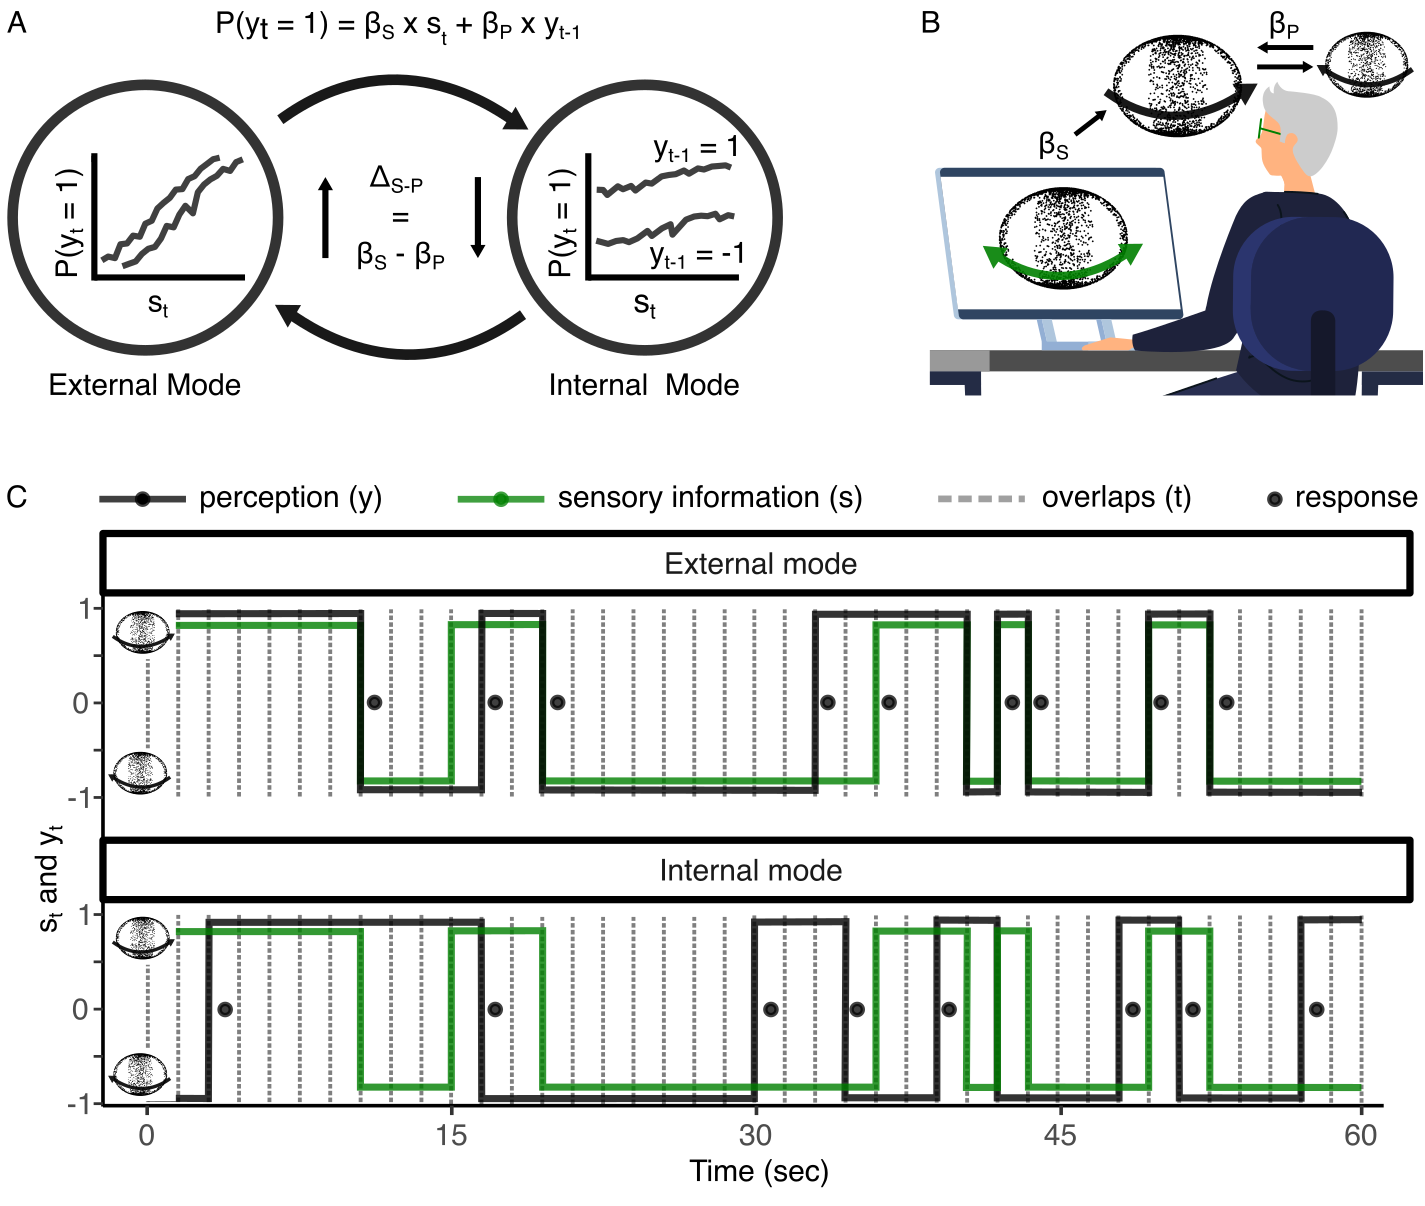
\includegraphics{./modes_ketamine_scz_files/figure-latex/Figure_1.png}

\textbf{Figure 1.}

\textbf{A.} Perception integrates ambiguous sensory signals \(s_t\) with
internal predictions that reflect prior knowledge about the world. One
source of prior knowledge is the temporal autocorrelation of natural
environments, where the recent past often predicts the near future. The
integration of external inputs and internal predictions depends on the
weights assigned to incoming sensory data (\(\beta_S \times s_t\)) and
to internal prediction derived from previous experiences
(\(\beta_P \times y_{t-1}\), dotted versus solid lines, simulated data),
respectively. \(\beta_S\) determines the slope, and \(\beta_P\) the
shift of the psychometric function that links \(s_t\) and \(y_t\).
Importantly, the balance \(\Delta_{S-P} = \beta_S - \beta_P\) is known
to alternate between two opposing modes: During the external mode
(left), perception is largely determined by \(\beta_S \times s_t\),
which is reflected by a steep slope and a small shift of the
psychometric curve. Conversely, during the internal mode (right),
perception is shaped by \(\beta_P \times y_{t-1}\), resulting in a
shallow slope and a large shift of the psychometric curve.

\textbf{B.} We conducted a double-blind placebo-controlled experiments
in 28 healthy human participants, who received a continuous infusion
with either the NMDAR antagonist S-ketamine or saline. During the
infusion, the participants viewed SFM stimuli at varying levels of
signal-to-ambiguity (SAR). The stimuli were compatible with two mutually
exclusive subjective experiences (left vs.~rightward rotation of the
front surface, green arrows). Fully ambiguous stimuli (SAR = 0) induce
the phenomenon of bistable perception, where participants perceive
spontaneous changes between the two possible interpretations of the
stimulus (black arrows) at a rate that is governed by \(\beta_P\), the
degree to which perception is shaped by internal predictions derived
from previous experiences. For partially ambiguous stimuli (SAR
\textgreater{} 0), perception reflects the weighted integration of
internal predictions with external sensory data, which is governed by
the balance \(\Delta_{S-P} = \beta_S - \beta_P\).

\textbf{C.} Changes in the perceived direction of rotation of the SFM
stimulus occur at brief depth-symmetric configurations of the stimulus
(overlaps, grey dotted lines; Supplemental Video S1). We transformed the
behavioral responses into a sequence of states \(t\) (1.5 sec intervals,
corresponding to the interval between consecutive overlaps), each
associated with a combination of the SAR-weighted input \(s_t\) (green
line) and the perceived direction of rotation \(y_t\) (black line).
Participants reported whenever they experienced a change in conscious
experience (black dots). The response times \(r_t\) was defined as the
lag between the response and the last preceding overlap. We used
HMM-GLMs to quantify the weights \(\beta_S\), \(\beta_P\) and
\(\beta_B\), which reflect how the reported percepts \(y_t\) were
determined by the external inputs \(\beta_S \times s_t\), the internal
predictions \(\beta_P \times y_{t-1}\), and the constant bias
\(\beta_B \times 1\), separately for the external mode (upper panel, 60
sec of example data) and the internal mode (lower panel, 60 sec of
example data with identical \(s(t)\) for visualization). In the external
mode, perception follows the external stimulus closely (high
\(\Delta_{S-P} = \beta_S - \beta_P\)). In the internal mode, perception
is shaped more strongly by internal predictions derived from previous
experiences (low \(\Delta_{S-P} = \beta_S - \beta_P\)).

\newpage

\subsection{Figure 2}\label{figure-2}

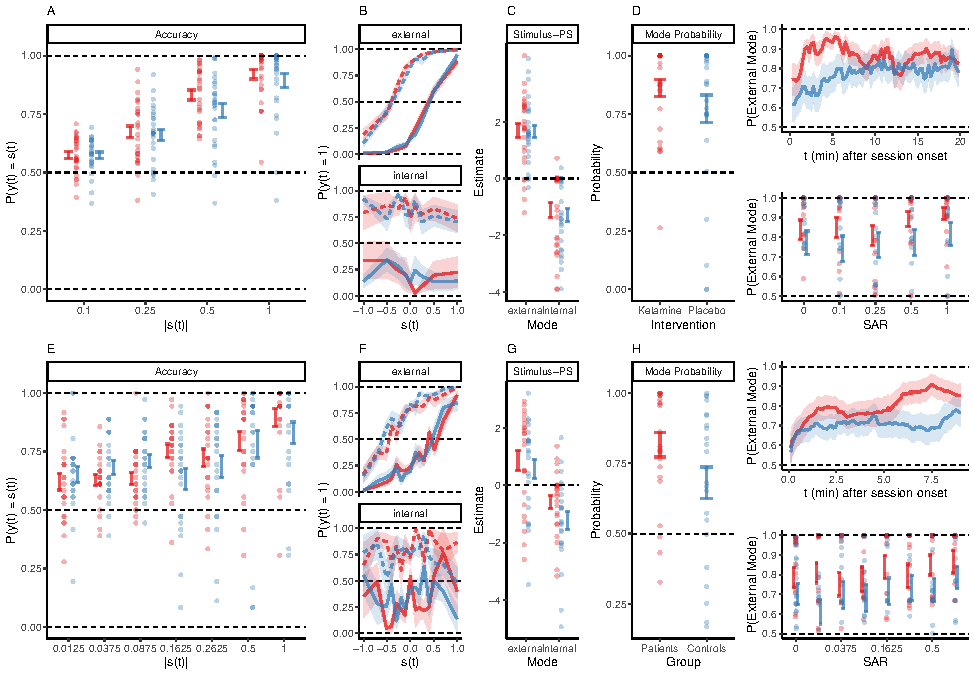
\includegraphics{modes_ketamine_scz_files/figure-latex/Figure_2-1.pdf}

\textbf{Figure 2.}

\textbf{A.} The percepts \(y_t\) were more likely to match the stimuli
\(s_t\) at higher levels of SAR (\(\beta\) = \(3.01\) ± \(0.06\), z =
\(50.39\), p = \(0\)). The positive effect of SAR on
\(P(y_t \cong s_t)\) was more pronounced under S-ketamine (red) relative
to placebo (blue; \(\beta\) = \(0.45\) ± \(0.08\), z = \(5.6\), p =
\(\ensuremath{1.71\times 10^{-7}}\)).

\textbf{B.} In the S-ketamine experiment, the HMM identified two modes
that differed with respect to the relative weighting of external sensory
data and internal predictions: Perception fluctuated between an external
mode, determined by the input \(s_t\) (upper panel panel, steep slope
and small shift of the psychometric curve), and an internal mode,
dominated by a stabilizing prediction that biased perception toward
previous experiences \(y_{t-1}\) (lower panel, shallow slope and large
shift of the psychometric curve). Within modes, there was no significant
effect of S-ketamine (red) versus placebo (blue) on the relation of
\(y(t)\) with \(s(t)\) and \(y(t-1)\).

\textbf{C.} \(\Delta_{S-P}\), the balance between the external input and
the stabilizing internal predictions, was larger during external than
during internal mode (\(\beta\) = \(2.8\) ± \(0.29\), T(\(-81\)) =
\(-9.5\), p = \(\ensuremath{5.22\times 10^{-13}}\)). Importantly, we
found no significant effect of S-ketamine (red) vs.~placebo (blue) on
\(\Delta_{S-P}\) within modes (\(\beta\) = \(-0.03\) ± \(0.29\),
T(\(81\)) = \(-0.1\), p = \(1\)).

\textbf{D.} S-ketamine (red) increased the probability of external mode
(\(\beta\) = \(1.01\) ± \(0.03\), z = \(30.7\), p =
\(\ensuremath{4.26\times 10^{-206}}\)) relative to placebo (blue). The
effect of S-ketamine on mode was present from the start of the session
(\(\beta\) = \(1.77\) ± \(0.07\), z = \(26.9\), p =
\(\ensuremath{3.55\times 10^{-158}}\), upper right panel), with no
significant effect of time (\(\beta\) = \(-0.18\) ± \(0.08\), z =
\(-2.17\), p = \(0.48\)). Relative to placebo, S-ketamine increased the
probability of external mode across all SARs (\(\beta\) = \(0.85\) ±
\(0.06\), z = \(14.14\), p = \(\ensuremath{3.33\times 10^{-44}}\), lower
right panel). Higher SARs were associated with an increased probability
of external mode (\(\beta\) = \(1.34\) ± \(0.09\), z = \(15.01\), p =
\(\ensuremath{9.97\times 10^{-50}}\)), in particular under S-ketamine
(\(\beta\) = \(0.62\) ± \(0.11\), z = \(5.52\), p =
\(\ensuremath{5.27\times 10^{-7}}\)). Alternations between external and
internal mode were found at all SARs: From from full ambiguity to
complete disambiguation, the probability of external mode increased by
only 0.11 under S-ketamine and 0.07 under placebo.

\textbf{E.} In patients (red) and controls (blue), percepts \(y_t\) were
more likely to match the stimuli \(s_t\) at higher levels of SAR
(\(\beta\) = \(2.77\) ± \(0.11\), z = \(24.85\), p =
\(\ensuremath{2.18\times 10^{-135}}\)). Patients followed the external
inputs more closely than controls (\(\beta\) = \(0.75\) ± \(0.15\), z =
\(4.96\), p = \(\ensuremath{5.6\times 10^{-6}}\)).

\textbf{F.} In analogy to the S-ketamine experiment, the HMM identified
two opposing modes in Scz patients (red) and controls (blue). The
external mode increased the sensitivity toward \(s_t\) (slope of the
psychometric function) and weakened the effect of the stabilizing
internal prediction \(y_{t-1}\) (shift between the dotted and solid
line) relative to the internal mode. Within modes, there was no effect
of group on the relation of \(y(t)\) with \(s(t)\) and \(y(t-1)\).

\textbf{G.} The external mode increased \(\Delta_{S-P}\), the balance
between external inputs and internal predictions, in patients (red) and
controls (blue; \(\beta\) = \(1.44\) ± \(0.33\), T(\(44\)) = \(4.33\), p
= \(\ensuremath{3.39\times 10^{-4}}\)), with no significant effect of
group (\(\beta\) = \(-0.28\) ± \(0.54\), T(\(87.97\)) = \(-0.52\), p =
\(1\)).

\textbf{H.} Relative to controls (blue), patients (red) spent more time
in external mode (\(\beta\) = \(0.52\) ± \(0.03\), z = \(16.88\), p =
\(\ensuremath{1.23\times 10^{-63}}\)). In both group, biases toward
external mode increased over time after session onset (\(\beta\) =
\(2.41\) ± \(0.11\), z = \(21.37\), p =
\(\ensuremath{4.07\times 10^{-100}}\); upper right panel), with a
stronger effect in patients (\(\beta\) = \(-1.84\) ± \(0.14\), z =
\(-12.97\), p = \(\ensuremath{2.83\times 10^{-37}}\)). Patients were
more likely than controls to be in external mode across all levels of
SAR (\(\beta\) = \(0.51\) ± \(0.03\), z = \(14.56\), p =
\(\ensuremath{7.57\times 10^{-47}}\), lower right panel). External mode
increased with SAR (\(\beta\) = \(0.63\) ± \(0.1\), z = \(6.47\), p =
\(\ensuremath{1.54\times 10^{-9}}\)), with no significant difference
between groups (\(\beta\) = \(0.15\) ± \(0.13\), z = \(1.16\), p =
\(1\)). As in the S-ketamine experiment, alternations between external
and internal mode were found at all SARs: From from full ambiguity to
complete disambiguation, the probability of external mode increased by
only 0.12 in patients and 0.18 in controls.

\newpage

\section{Supplemental Information}\label{supplemental-information}

\subsection{Supplemental Figure S1}\label{supplemental-figure-s1}

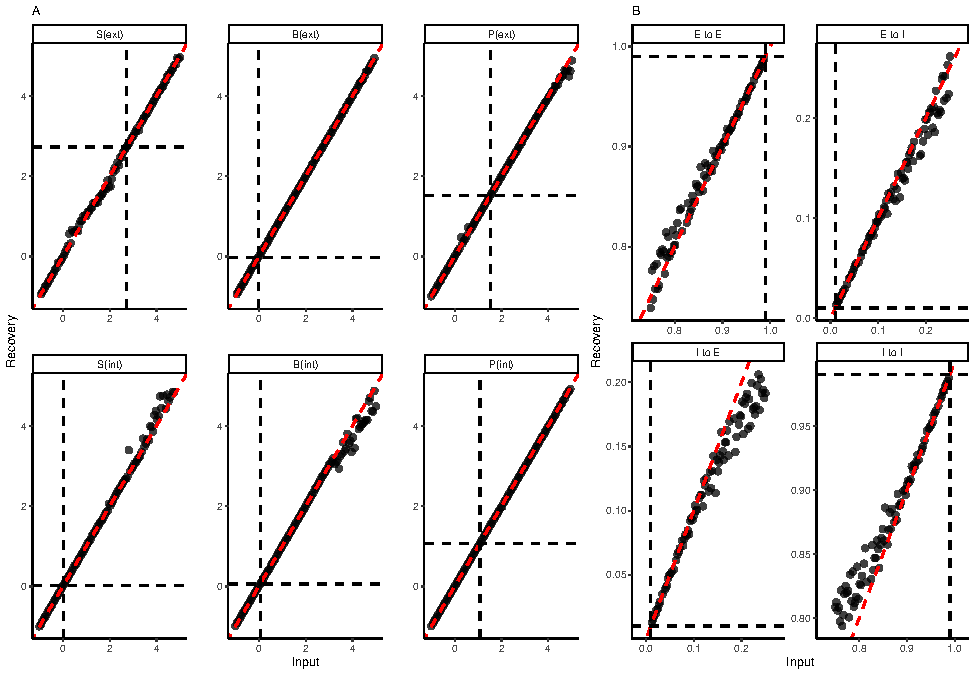
\includegraphics{modes_ketamine_scz_files/figure-latex/Supplemental_Figure_S1-1.pdf}
\textbf{Supplemental Figure S1. GLM-HMM parameter recovery}

\textbf{A}. Weight recovery from simulated data: GLM weights. The
GLM-HMM is defined by the mode-dependent weights \(\beta_S\),
\(\beta_B\), and \(\beta_P\). To test how well our GLM-HMM can recover
changes in individual weights, we selected one of the six weights (3
weights x 2 modes) and varied its value parametrically from -1 to 5. For
each inversion, we kept all other weights at the group-level average
obtained from the original data. For each of the six recovery analyses,
we simulated synthetic experiences \(y_{syn}\) for n = 78400 overlaps
(number of overlaps across participants in the S-ketamine experiment).
We then fitted a randomly initialized GLM-HMM to the synthetic
experiences, and extracted the weights recovered from the synthetic
experiences \(y_{syn}\). We performed each recovery for 10 iterations,
computed the average posterior weights \(\beta_S\), \(\beta_B\), and
\(\beta_P\), and correlated them with the synthetic input weights. The
correlation with the parametric input weights and the posterior weights
recovered from the simulated data were close to 1 for all weights
(\(\beta_S\), \(\beta_B\), and \(\beta_P\), columns) and modes (external
and internal, rows). Weights were recovered with high fidelity across a
broad range of weights (average r = 0.99), and in particular at the
group-level weights \(w_n\) obtained from the original data (black
dotted line). The red dashed line represents the identity line (slope =
1, intercept = 0), indicating perfect recovery.

\textbf{B}. Weight recovery from simulated data: transition matrix. We
repeated the above procedure for each cell of the GLM-HMM transition
matrix. We initialized models with parametric transition probabilities
ranging from 0.8 to 1 (on-diagonal cells, external to external, internal
to internal) and 0 to 0.2 (off-diagonal cells, external to internal,
internal to external). Transition probabilities were recovered with high
fidelity across a broad range of parameters (average r = 0.99), and in
particular at the group-level estimates obtained from the original data
(black dotted line). The red dashed line represents the identity line
(slope = 1, intercept = 0), indicating perfect recovery.

\newpage

\subsection{Supplemental Figure S2}\label{supplemental-figure-s2}

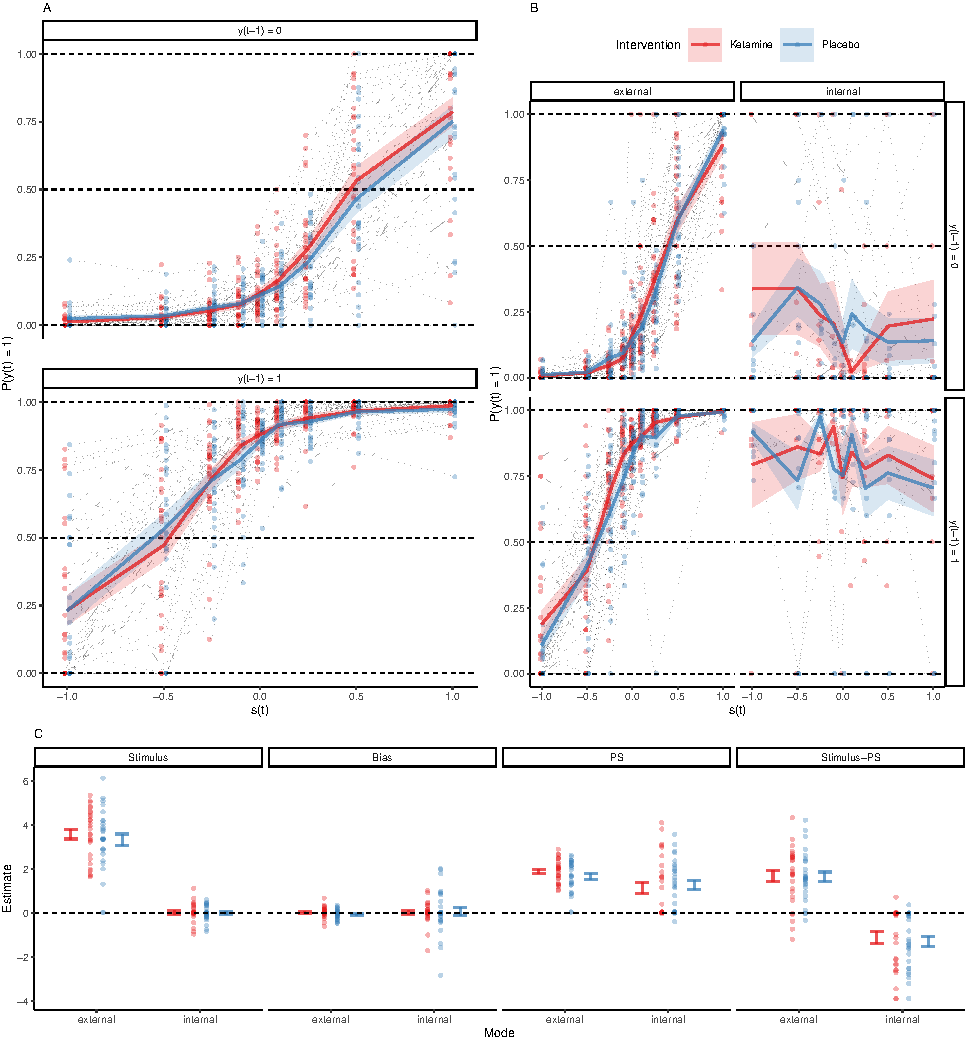
\includegraphics{modes_ketamine_scz_files/figure-latex/Supplemental_Figure_S2-1.pdf}

\textbf{Supplemental Figure S2. The effects of ketamine and bimodal
inference on RT.}

\textbf{A.} RT were non-uniformly distributed across the inter-overlap
interval (D = \(0.09\), p = \(\ensuremath{5.38\times 10^{-9}}\),
one-sample Kolmogorov-Smirnov test). This corroborates that changes in
perception aligned with the overlapping configurations of the stimulus
after S-ketamine (red) and placebo (blue).

\textbf{B.} RT showed a quadratic relationship with \(s_t\) (\(\beta\) =
\(-6.87\) ± \(1.68\), T(\(\ensuremath{6.2\times 10^{3}}\)) = \(-4.1\), p
= \(\ensuremath{5.1\times 10^{-4}}\)), indicating faster responses when
sensory information was reliable (\(|s_t| \gg  0\); note that SAR as
shown in Figure 2A and 2E is equal to \(|s_t|\)). We observed no main
effect of S-ketamine (red) vs.~placebo (blue) on RT (\(\beta\) =
\(\ensuremath{-3.35\times 10^{-3}}\) ± \(0.01\),
T(\(\ensuremath{6.2\times 10^{3}}\)) = \(-0.32\), p = \(1\)).

\textbf{C.} We found no additional effect of mode on RT (\(\beta\) =
\(0.02\) ± \(0.03\), z = \(\ensuremath{5.96\times 10^{3}}\), p =
\(0.78\)).

\textbf{D.} Confidence showed a quadratic relationship with \(s_t\)
(\(\beta\) = \(74.83\) ± \(2.39\), z = \(31.32\), p =
\(\ensuremath{3.22\times 10^{-214}}\)), confirming that participants
were more confident when sensory information was reliable
(\(|s_t| = SAR \gg  0\)). Relative to placebo (blue), S-ketamine (red)
reduced choice confidence (\(\beta\) = \(-0.21\) ± \(0.04\), z =
\(-5.9\), p = \(\ensuremath{4.36\times 10^{-8}}\)), and decreased the
quadratic effect of \(s_t\) on confidence (\(\beta\) = \(-19.95\) ±
\(2.36\), z = \(-8.45\), p = \(\ensuremath{3.48\times 10^{-16}}\)).

\textbf{E.} External mode increased confidence globally (\(\beta\) =
\(0.72\) ± \(0.07\), z = \(9.92\), p =
\(\ensuremath{7.85\times 10^{-22}}\)) and by elevating the quadratic
effect of \(s_t\) on confidence (\(\beta\) = \(242.61\) ± \(18.43\), z =
\(13.16\), p = \(\ensuremath{3.37\times 10^{-38}}\)). When controlling
for mode, the negative effect of S-ketamine (red) vs.~placebo (blue) on
confidence and on the quadratic relationship of confidence with \(s_t\)
remained significant.

\newpage

\subsection{Supplemental Figure S3}\label{supplemental-figure-s3}

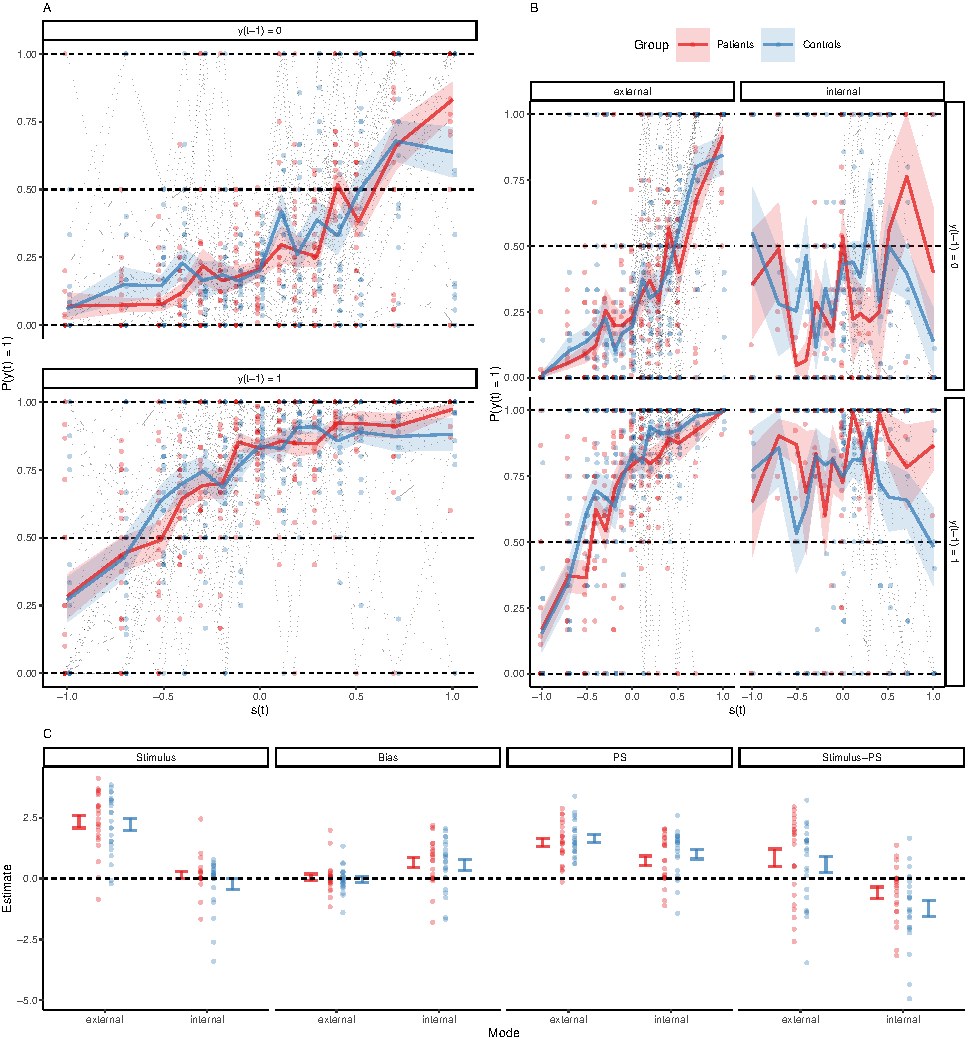
\includegraphics{modes_ketamine_scz_files/figure-latex/Supplemental_Figure_S3-1.pdf}

\textbf{Supplemental Figure S3. Extended data on the effects of
S-ketamine and mode on perceptual inference (related to Figure 2A-C).}

\textbf{A.} Here, we show psychometric curves (percept \(y_t\) versus
input \(s_t\)) under S-ketamine (red) and placebo (blue). The plot
separates times \(t\) for which the previous experience was leftward
rotation (\(y_{t-1} = -1\), upper panel) and rightward rotation
(\(y_{t-1} = +1\), lower panel). As expected, \(y_t\) was driven by both
the external input \(s_t\) (\(\beta_S\) = \(3.01\) ± \(0.06\), z =
\(50.39\), p = \(0\)) and the previous percept \(y_{t-1}\)
(\(\beta_{P}\) = \(2.06\) ± \(0.03\), z = \(80.58\), p = \(0\)). We
found no significant interaction between the \(s_t\) and \(y_{t-1}\)
(\(\beta\) = \(-0.06\) ± \(0.06\), z = \(-1.06\), p = \(1\)). Relative
to placebo, S-ketamine caused a shift of \(y_t\) toward \(s_t\)
(\(\beta\) = \(0.45\) ± \(0.08\), z = \(5.6\), p =
\(\ensuremath{1.71\times 10^{-7}}\)), with no significant effect on
\(y_{t-1}\) (\(\beta\) = \(0.08\) ± \(0.04\), z = \(2.39\), p =
\(0.13\)). We found no significant three-way-interaction (drug x \(s_t\)
x \(y_{t-1}\), \(\beta\) = \(-0.07\) ± \(0.08\), z = \(-0.9\), p =
\(1\)).

\textbf{B.} This panel shows the data from panel (A) separately for
times \(t\) where the HMM identified the mode of perceptual inference as
external (left panels) or internal (right panels). When the mode of
perceptual processing was added to the prediction of \(y_t\) from
\(s_t\) and \(y_{t-1}\), the effect S-ketamine (red) vs.~placebo (blue)
on \(s_t\) disappeared (\(\beta\) = \(0.24\) ± \(0.11\), z = \(2.13\), p
= \(0.53\)). Instead, changes in the balance between \(s_t\) and
\(y_{t-1}\) were loaded onto fluctuations between external and internal
mode, which caused perception to shift away from external inputs \(s_t\)
(\(\beta\) = \(-4.23\) ± \(0.21\), z = \(-20.01\), p =
\(\ensuremath{7.54\times 10^{-88}}\)) and toward previous experiences
\(y{t-1}\) (\(\beta\) = \(0.78\) ± \(0.09\), z = \(8.64\), p =
\(\ensuremath{8.81\times 10^{-17}}\)).

\textbf{C.} Here, we plot the weights from the GLM
\(y_t = \beta_S \times s_t + \beta_P \times y_{t-1} + \beta_B \times 1\),
alongside the balance between external inputs and previous experiences
\(\Delta_{S-P} = \beta_S - \beta_P\) during external and internal mode.
Colors indicate S-ketamine (red) and placebo (blue). \(\beta_S\), the
weight associated with the external input \(s_t\), was positive in
external mode, but reduced to zero in internal mode (\(\beta\) =
\(-3.55\) ± \(0.23\), T(\(81\)) = \(-15.44\), p =
\(\ensuremath{4.78\times 10^{-24}}\)). We found no additional effect of
S-ketamine (red) versus placebo (blue; \(\beta\) = \(-0.25\) ± \(0.23\),
T(\(81\)) = \(-1.1\), p = \(1\)) and no significant interaction
(\(\beta\) = \(0.21\) ± \(0.33\), T(\(81\)) = \(0.65\), p = \(1\)).
\(\beta_B\), the weight associated with the constant response bias \(b\)
toward rightward rotation, was not different from zero (\(\beta_B\) =
\(0.04\) ± \(0.11\), T(\(98.36\)) = \(0.31\), p = \(1\)). We found no
effect of drug (\(\beta\) = \(-0.11\) ± \(0.14\), T(\(81\)) = \(-0.74\),
p = \(1\)) or mode (\(\beta\) = \(-0.02\) ± \(0.14\), T(\(81\)) =
\(-0.12\), p = \(1\)) on the bias weight \(\beta_B\). \(\beta_P\), the
weight associated with the previous percept \(y_{t-1}\) was not
modulated by S-ketamine (\(\beta\) = \(-0.22\) ± \(0.26\), T(\(81\)) =
\(-0.87\), p = \(1\)) or mode (\(\beta\) = \(-0.75\) ± \(0.26\),
T(\(81\)) = \(-2.92\), p = \(0.29\)). There was no significant
interaction between drug and mode with respect to \(\beta_P\) (\(\beta\)
= \(0.35\) ± \(0.36\), T(\(81\)) = \(0.97\), p = \(1\)). The balance
\(\Delta_{S-P}\) between external inputs and internal predictions was
determined by mode (\(\beta\) = \(2.8\) ± \(0.29\), T(\(81\)) = \(9.5\),
p = \(\ensuremath{5.22\times 10^{-13}}\)), with no significant effect of
S-ketamine (\(\beta\) = \(0.03\) ± \(0.29\), T(\(81\)) = \(0.1\), p =
\(1\)) and no interaction (\(\beta\) = \(0.14\) ± \(0.42\), T(\(81\)) =
\(0.34\), p = \(1\)). These posterior GLM-HMM weights argue against the
alternative hypotheses that the primary effect of S-ketamine is related
to changes in dynamics of bias (state 1: high \(\beta_B\); state 2: low
\(\beta_B\); hypothesis H3) or the randomness of experience (state 1:
high \(\beta_S\) and \(\beta_P\); state 2: low \(\beta_S\) and
\(\beta_P\) with no difference in \(\Delta_{S-P}\) between modes:
hypothesis H4).

\textbf{D.} S-ketamine (red) increased the probability of external mode
(\(\beta\) = \(1.01\) ± \(0.03\), z = \(30.7\), p =
\(\ensuremath{4.26\times 10^{-206}}\)) relative to placebo (blue) by
elevating the stability of external at the expense of internal mode (EE
versus II; left panels; V = 264, p = 0.01), with no effect on the
transition probabilities between modes (EI versus IE; right panels; V =
149, p = 0.37).

\newpage

\subsection{Supplemental Figure S4}\label{supplemental-figure-s4}

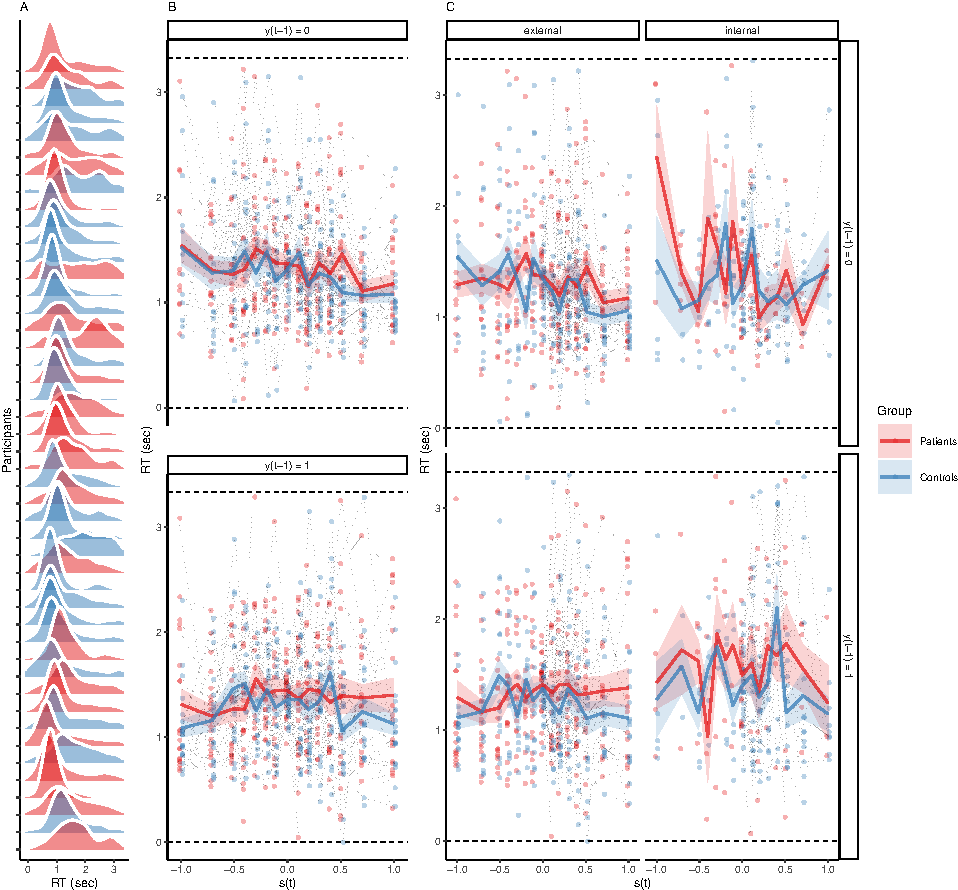
\includegraphics{modes_ketamine_scz_files/figure-latex/Supplemental_Figure_S4-1.pdf}

\textbf{Supplemental Figure S4. Extended data on external and internal
mode in Scz patients and healthy controls (related to Figure 2E-H).}

\textbf{A.} Here, we show psychometric curves (percept \(y_t\) versus
input \(s_t\)) in patients (red) and controls (blue). The plot separates
times \(t\) for which the previous experience was leftward rotation
(\(y_{t-1} = -1\), upper panel) and rightward rotation
(\(y_{t-1} = +1\), lower panel). Perception was driven by \(s_t\)
(\(\beta_S\) = \(2.77\) ± \(0.11\), z = \(24.85\), p =
\(\ensuremath{2.18\times 10^{-135}}\)) and \(y_{t-1}\) (\(\beta_{P}\) =
\(1.5\) ± \(0.03\), z = \(58.2\), p = \(0\)), with no significant
interaction between \(s_t\) and \(y_{t-1}\) (\(\beta\) =
\(\ensuremath{-5.41\times 10^{-3}}\) ± \(0.11\), z = \(-0.05\), p =
\(1\)). Patients were more sensitive to \(s_t\) (\(\beta\) = \(0.75\) ±
\(0.15\), z = \(4.96\), p = \(\ensuremath{5.6\times 10^{-6}}\)). We
found no significant three-way-interaction (group x \(s_t\) x
\(y_{t-1}\), \(\beta\) = \(-0.37\) ± \(0.15\), z = \(-2.45\), p =
\(0.11\)).

\textbf{B.} This panel shows the data from panel (A) separately for
times \(t\) where the HMM identified the mode of perceptual inference as
external (left panels) or internal (right panels). When the mode of
perceptual processing was added to the prediction of \(y_t\) from
\(s_t\) and \(y_{t-1}\), the difference between patients (red) and
controls (blue) in the effect of \(s_t\) on \(y_t\) disappeared
(\(\beta\) = \(-0.02\) ± \(0.22\), z = \(-0.08\), p = \(1\)). Instead,
changes in the balance between \(s_t\) and \(y_{t-1}\) were loaded onto
fluctuations between external and internal mode, which caused perception
to shift away from external inputs \(s_t\) (\(\beta\) = \(-3.47\) ±
\(0.29\), z = \(-11.95\), p = \(\ensuremath{1.01\times 10^{-31}}\)) and
toward previous experiences \(y{t-1}\) (\(\beta\) = \(0.5\) ± \(0.07\),
z = \(6.85\), p = \(\ensuremath{1.15\times 10^{-10}}\)).

\textbf{C.} Here, we plot the weights from the GLM
\(y_t = \beta_S \times s_t + \beta_P \times y_{t-1} + \beta_B \times 1\),
alongside the balance between external inputs and previous experiences
\(\Delta_{S-P} = \beta_S - \beta_P\) during external and internal mode.
Colors indicate the group (patients in red, controls in blue).
\(\beta_S\), the weight associated with the external input \(s_t\), was
positive in external mode, but reduced to zero in internal mode
(\(\beta\) = \(-2.19\) ± \(0.24\), T(\(44\)) = \(-9.13\), p =
\(\ensuremath{4.07\times 10^{-11}}\)). We found no additional effect of
group (\(\beta\) = \(-0.11\) ± \(0.37\), T(\(87.69\)) = \(-0.3\), p =
\(1\)) and no significant interaction (\(\beta\) = \(-0.25\) ± \(0.34\),
T(\(44\)) = \(-0.74\), p = \(1\)). \(\beta_B\), the weight associated
with the constant response bias \(b\) toward rightward rotation, was not
different from zero (\(\beta\) = \(0.05\) ± \(0.18\),
T(\(\ensuremath{1.62\times 10^{-8}}\)) = \(0.29\), p = \(1\)). We found
no effect of group (\(\beta\) = \(-0.09\) ± \(0.25\),
T(\(\ensuremath{1.62\times 10^{-8}}\)) = \(-0.37\), p = \(1\)). There
was a trend for a positive effect of internal mode (\(\beta\) = \(0.6\)
± \(0.24\), T(\(88\)) = \(2.47\), p = \(0.06\)) on the bias weight
\(\beta_B\). \(\beta_P\), the weight associated with the previous
percept \(y_{t-1}\), was reduced in internal mode (\(\beta\) = \(-0.75\)
± \(0.26\), T(\(88\)) = \(-2.92\), p = \(0.02\)), but not modulated by
group (\(\beta\) = \(0.17\) ± \(0.32\),
T(\(\ensuremath{9.88\times 10^{-10}}\)) = \(0.54\), p = \(1\)). There
was no significant interaction between group and mode with respect to
\(\beta_P\) (\(\beta\) = \(0.11\) ± \(0.36\), T(\(88\)) = \(0.3\), p =
\(1\)). The balance \(\Delta_{S-P}\) between external inputs and
internal predictions was determined by mode (\(\beta\) = \(1.44\) ±
\(0.33\), T(\(81\)) = \(9.5\), p = \(\ensuremath{3.39\times 10^{-4}}\)),
with no significant effect of group (\(\beta\) = \(0.28\) ± \(0.54\),
T(\(87.97\)) = \(0.52\), p = \(1\)) and no interaction (\(\beta\) =
\(0.36\) ± \(0.47\), T(\(44\)) = \(0.76\), p = \(1\)). These posterior
GLM-HMM weights argue against the alternative hypotheses that the
primary effect of S-ketamine is related to changes in dynamics of bias
(state 1: high \(\beta_B\); state 2: low \(\beta_B\); hypothesis H3) or
the randomness of experience (state 1: high \(\beta_S\) and \(\beta_P\);
state 2: low \(\beta_S\) and \(\beta_P\) with no difference in
\(\Delta_{S-P}\) between modes: hypothesis H4).

\textbf{D.} Relative to controls (blue), patients (red) spent more time
in external mode (\(\beta\) = \(0.52\) ± \(0.03\), z = \(16.88\), p =
\(\ensuremath{1.23\times 10^{-63}}\)). This effect was driven by an
increase in the stability of external mode at the expense of internal
mode (EE versus II; left panels; W = 352, p = 0.03). There was no effect
of group on the transition probabilities between modes (EI versus IE;
right panels; W = 248, p = 0.65).

\newpage

\subsection{Supplemental Figure S5}\label{supplemental-figure-s5}

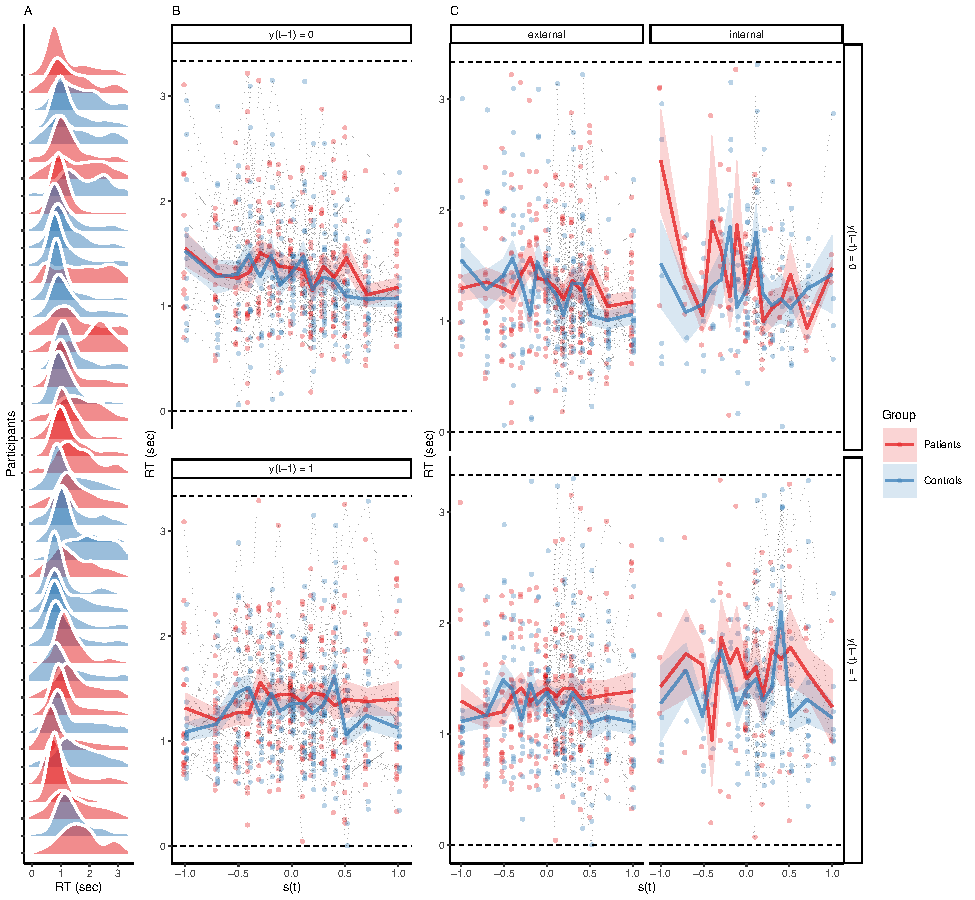
\includegraphics{modes_ketamine_scz_files/figure-latex/Supplemental_Figure_S5-1.pdf}

\textbf{Supplemental Figure S5. RT and bimodal inference in Scz patients
and controls.}

\textbf{A.} RT were non-uniformly distributed across the inter-overlap
interval (D = \(0.22\), p = \(\ensuremath{2.39\times 10^{-232}}\),
one-sample Kolmogorov-Smirnov test against uniformity) in patients (red)
and controls (blue). This confirmed that changes in perception were
aligned with the overlapping configurations of the stimulus.

\textbf{B.} RT did not differ between patients (red) and controls (blue;
\(\beta\) = \(-0.07\) ± \(0.08\), T(\(66.96\)) = \(-0.87\), p = \(1\)).
We found no quadratic relationship between RT and \(s_t\) (\(\beta\) =
\(-3.54\) ± \(2.34\), T(\(\ensuremath{5.33\times 10^{3}}\)) = \(-1.51\),
p = \(1\)).

\textbf{C.} We found no effect of mode on RT (\(\beta\) = \(0.03\) ±
\(0.04\), z = \(\ensuremath{4.89\times 10^{3}}\), p = \(0.76\)).

\newpage

\subsection{Supplemental Figure S6}\label{supplemental-figure-s6}

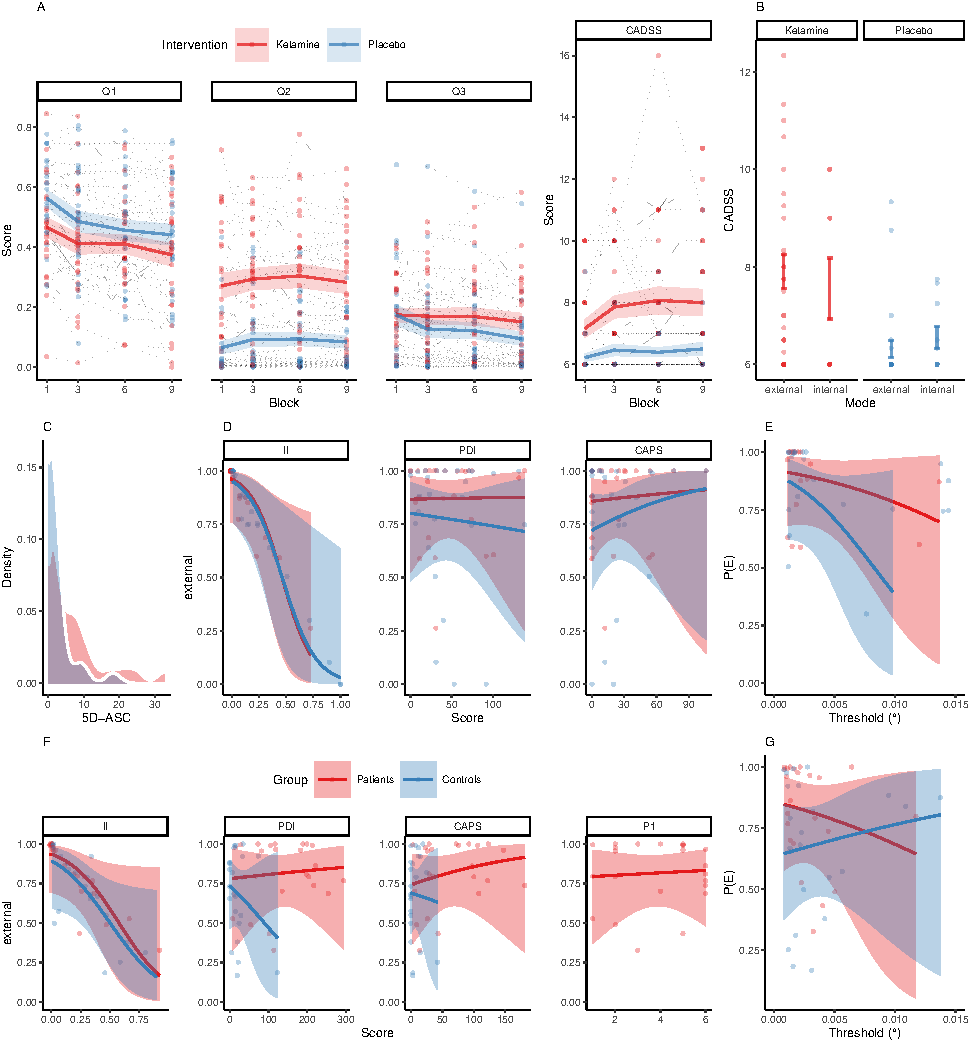
\includegraphics{modes_ketamine_scz_files/figure-latex/Supplemental_Figure_S6-1.pdf}

\textbf{Supplemental Figure S6. Scores and Questionnaires.}

\textbf{A.} Responses to Q1 (\emph{How awake do you feel?}) indicated
that participants felt more tired under S-ketamine (red) than placebo
(blue; \(\beta\) = \(-1.53\) ± \(0.6\), z = \(-2.57\), p = \(0.04\)),
with no significant effect of time or a between-factor interaction.
Responses to Q2 (\emph{How intoxicated do you feel?}) indicated that
participants felt more intoxicated under S-ketamine (\(\beta\) =
\(3.32\) ± \(1.44\), z = \(2.3\), p = \(0.09\)), with no significant
effect of time or a between-factor interaction. Responses to Q3
(\emph{How nervous do you feel?}) revealed no effect of S-ketamine
(\(\beta\) = \(-3.01\) ± \(2.62\), z = \(-1.15\), p = \(1\)), time, nor
a significant between-factor interaction. CADSS scores were elevated
under S-ketamine (\(\beta\) = \(1.01\) ± \(0.34\), T(\(185.32\)) =
\(2.99\), p = \(0.01\)) with a borderline trend for an increase over
time (\(0.09\) ± \(0.04\), T(\(185.61\)) = \(2.24\), p = \(0.1\)) and no
significant between-factor interaction.

\textbf{B.} Q1-3 and CADSS scores were collected after blocks 1, 3, 6
and 9. To assess how the mode of perceptual inference was linked to
dissociative symptoms, we separated the participants ratings according
to the mode that dominated perception at the very end of the preceding
block. While controlling the effect of S-ketamine (red) vs placebo
(blue), we found that external mode increased dissociative symptoms
(\(\beta\) = \(1.05\) ± \(0.54\), T(\(208.05\)) = \(1.95\), p =
\(0.05\)), but had no effect on wakefulness (Q1), subjective
intoxication (Q2) or nervousness (Q3).

\textbf{C.} 5-ASC scores were elevated under S-ketamine (red) relative
to placebo (blue; \(\beta\) = \(4.89\) ± \(1.59\), T(\(27.14\)) =
\(3.08\), p = \(\ensuremath{9.33\times 10^{-3}}\)).

\textbf{D.} Neither PDI, CAPS, nor 5-ASC scores were predictive of the
probability of external mode (shown separately for S-ketamine in red and
placebo in blue).

\textbf{E.} Stereodisparity thresholds were not predictive of the
probability of external mode (\(\beta\) = \(-28.73\) ± \(781.1\), z =
\(-0.04\), p = \(0.97\)). Thresholds did not differ between S-ketamine
(red) and placebo (blue; W = \(102\), p = \(0.66\)).

\textbf{F.} Neither PDI, CAPS (patients in red and controls in blue),
nor the PANSS items P1 (delusions) or P3 (hallucinations, patients only)
predicted the probability of external mode.

\textbf{G.} In patients (red) and controls (blue), stereodisparity
thresholds were not predictive of the probability of external mode
(\(\beta\) = \(-1.88\) ± \(2.05\), z = \(-0.92\), p = \(1\)). Thresholds
did not differ between groups (V = \(976\), p = \(0.52\)).

\newpage

\subsection{Supplemental Table S1}\label{supplemental-table-s1}

\begin{longtable}[]{@{}
  >{\raggedright\arraybackslash}p{(\columnwidth - 4\tabcolsep) * \real{0.3148}}
  >{\raggedright\arraybackslash}p{(\columnwidth - 4\tabcolsep) * \real{0.4537}}
  >{\raggedright\arraybackslash}p{(\columnwidth - 4\tabcolsep) * \real{0.2315}}@{}}
\toprule\noalign{}
\begin{minipage}[b]{\linewidth}\raggedright
RESOURCE
\end{minipage} & \begin{minipage}[b]{\linewidth}\raggedright
SOURCE
\end{minipage} & \begin{minipage}[b]{\linewidth}\raggedright
IDENTIFIER
\end{minipage} \\
\midrule\noalign{}
\endhead
\bottomrule\noalign{}
\endlastfoot
\textbf{Deposited data \& code} & & \\
Analyzed data \& custom code &
\url{https://github.com/veithweilnhammer/modes_ketamine_scz/} & N/A \\
\textbf{Software} & & \\
\textbf{Matlab} & \url{https://www.mathworks.com/} & RRID:SCR\_001622 \\
Psychtoolbox 3 & \url{http://psychtoolbox.org/} & RRID:SCR\_002881 \\
\textbf{R} & \url{http://www.r-project.org/} & RRID:SCR\_001905 \\
RStudio & \url{https://www.rstudio.com/} & RRID:SCR\_000432 \\
lme4, afex, statConfR, ggplot2, ggridges, gridExtra, tidyr, plyr, readxl
& \url{http://cran.r-project.org/} & RRID:SCR\_003005 \\
\textbf{Python 3} & \url{http://www.python.org/} & RRID:SCR\_008394 \\
Jupyter Notebook & \url{https://jupyter.org/} & RRID:SCR\_018315 \\
numpy & \url{http://www.numpy.org} & RRID:SCR\_008633 \\
pandas & \url{https://pandas.pydata.org} & RRID:SCR\_018214 \\
SSM & \url{https://github.com/lindermanlab/ssm} & N/A \\
\end{longtable}

\textbf{Supplemental Table S1. Key resources.}

\newpage

\subsection{Supplemental Table S2}\label{supplemental-table-s2}

\begin{longtable}[]{@{}
  >{\raggedright\arraybackslash}p{(\columnwidth - 6\tabcolsep) * \real{0.1818}}
  >{\raggedright\arraybackslash}p{(\columnwidth - 6\tabcolsep) * \real{0.4364}}
  >{\raggedright\arraybackslash}p{(\columnwidth - 6\tabcolsep) * \real{0.1818}}
  >{\raggedright\arraybackslash}p{(\columnwidth - 6\tabcolsep) * \real{0.2000}}@{}}
\toprule\noalign{}
\begin{minipage}[b]{\linewidth}\raggedright
Scale
\end{minipage} & \begin{minipage}[b]{\linewidth}\raggedright
Scope
\end{minipage} & \begin{minipage}[b]{\linewidth}\raggedright
Condition
\end{minipage} & \begin{minipage}[b]{\linewidth}\raggedright
mean ± s.e.m.
\end{minipage} \\
\midrule\noalign{}
\endhead
\bottomrule\noalign{}
\endlastfoot
\textbf{PDI}\textsuperscript{29} & Delusion proneness & Global & 46.22 ±
7.19 \\
\textbf{CAPS}\textsuperscript{30} & Hallucination proneness & Global &
23 ± 5.05 \\
\textbf{BPRS}\textsuperscript{31} & Screen for psychotic illness &
Global & 0.64 ± 0.27 \\
\textbf{5D-ASC}\textsuperscript{35} & Altered states of consciousness &
S-ketamine & 7.11 ± 1.59 \\
& & Placebo & 2.2 ± 0.75 \\
\textbf{CADSS}\textsuperscript{34} & Dissociation & S-ketamine & 7.8 ±
0.33 \\
& & Placebo & 6.43 ± 0.17 \\
\textbf{Q1} & Wakefulness & S-ketamine & 0.41 ± 0.03 \\
& & Placebo & 0.48 ± 0.03 \\
\textbf{Q2} & Intoxication & S-ketamine & 0.29 ± 0.03 \\
& & Placebo & 0.09 ± 0.02 \\
\textbf{Q3} & Nervousness & S-ketamine & 0.17 ± 0.02 \\
& & Placebo & 0.13 ± 0.03 \\
\textbf{Stereovision} & Disparity thresholds & S-ketamine &
\ensuremath{2.89\times 10^{-3}} ± \ensuremath{6.18\times 10^{-4}} \\
& & Placebo & \ensuremath{2.75\times 10^{-3}} ±
\ensuremath{4.39\times 10^{-4}} \\
\end{longtable}

\textbf{Supplemental Table S2. Psychometric data for the S-ketamine
experiment.}

\newpage

\subsection{Supplemental Table S3}\label{supplemental-table-s3}

\begin{longtable}[]{@{}
  >{\raggedright\arraybackslash}p{(\columnwidth - 6\tabcolsep) * \real{0.1818}}
  >{\raggedright\arraybackslash}p{(\columnwidth - 6\tabcolsep) * \real{0.4364}}
  >{\raggedright\arraybackslash}p{(\columnwidth - 6\tabcolsep) * \real{0.1818}}
  >{\raggedright\arraybackslash}p{(\columnwidth - 6\tabcolsep) * \real{0.2000}}@{}}
\toprule\noalign{}
\begin{minipage}[b]{\linewidth}\raggedright
Scale
\end{minipage} & \begin{minipage}[b]{\linewidth}\raggedright
Scope
\end{minipage} & \begin{minipage}[b]{\linewidth}\raggedright
Condition
\end{minipage} & \begin{minipage}[b]{\linewidth}\raggedright
mean ± s.e.m.
\end{minipage} \\
\midrule\noalign{}
\endhead
\bottomrule\noalign{}
\endlastfoot
\textbf{PDI}\textsuperscript{29} & Delusion proneness & Patients &
138.83 ± 16.64 \\
& & Controls & 21.87 ± 5.75 \\
\textbf{CAPS}\textsuperscript{30} & Hallucination proneness & Patients &
65.17 ± 10.56 \\
& & Controls & 7.13 ± 2.2 \\
\textbf{P1} & Delusions & Patients & 3.83 ± 0.39 \\
\textbf{P3} & Delusions & Patients & 3.35 ± 0.44 \\
\textbf{Stereovision} & Disparity thresholds & Patients &
\ensuremath{2.82\times 10^{-3}} ± \ensuremath{5.13\times 10^{-4}} \\
& & Controls & \ensuremath{3.46\times 10^{-3}} ±
\ensuremath{7.14\times 10^{-4}} \\
\end{longtable}

\textbf{Supplemental Table S3. Psychometric data for Scz-control-study.}

\newpage

\section{Review v1}\label{review-v1}

We would like to thank the referees and the editorial team at Brain for
the very helpful and constructive review of our work. In response to the
comments raised by the editors and the reviewers, we have fundamentally
revised our manuscript. In particular, we have extended the introduction
and discussion to provide more links to the existing literature on
predictive processing, circular inference, and trait-versus-state. We
now show robust parameter recovery in the GLM-HMM framework, and provide
additional control analyses that support the hypothesis that external
and internal modes are perceptual as opposed to high-level behavioral or
cognitive phenomena. We hope that with these changes, our manuscript can
be accepted for publication in Brain.

Please find our point-by-point responses below. All changes are
highlighted in BOLD font in the main manuscript.

\subsection{Editorial comments}\label{editorial-comments}

We have changed the format of our paper to adhere with the Brain article
template we received. We have separated the \emph{Main} section of our
previous version in \emph{Introduction}, \emph{Results}, and
\emph{Discussion}. The \emph{Method} section now appears after the
\emph{Introduction}. These required two minor changes to the text of the
manuscript, which are highlighted in the revised manuscript:

We added a brief summary of our methods, results, and interpretation at
the end of the introduction:

\begin{itemize}
\tightlist
\item
  The objective of the current study was therefore twofold: First, to
  test whether NMDAR hypofunction causes changes in perceptual inference
  that characterize Scz; and second, to explore the effect of NMDAR
  hypofunction on ongoing fluctuations in perceptual inference that may
  explain the transient nature of psychotic experiences. We addressed
  these questions in a double-blind, placebo-controlled, cross-over
  experiment with S-ketamine in healthy participants, and a case-control
  study that compared patients with paranoid Scz to matched healthy
  controls\textsuperscript{28}. Participants engaged in a task designed
  to test how internal predictions derived from previous experiences
  modulate the perception of sensory signals that varied in ambiguity.
  We found that NMDAR antagonism and Scz were associated with a shift of
  perception toward the external mode, a minute-long state of the brain
  during which inference dissociates from prior knowledge. Our results
  suggest that NMDAR hypofunction shifts the balance between external
  and internal modes, and may thus contribute to the symptoms of Scz by
  causing transient and recurring failures of perceptual inference.
\end{itemize}

At the beginning of the discussion, we have added a brief summary of our
findings:

\begin{itemize}
\tightlist
\item
  Perception integrates incoming signals with internal predictions that
  reflect prior knowledge about the world\textsuperscript{4}. Our
  results indicate that this integration is subject to dynamic changes
  over time, alternating between an external mode, where perception
  closely follows the external input, and an internal mode, where
  perception is shaped by internal
  predictions\textsuperscript{26,55,56}. The internal mode enables the
  brain to use prior knowledge about the statistics of natural
  environment, such as their temporal autocorrelation, for efficient
  perception\textsuperscript{26}. Intermittent episodes of external mode
  processing decouple perception from prior knowledge. The balance
  between external and internal mode may prevent circular inferences
  within recurrent neural networks, where predictive feedback influences
  early sensory processing stages\textsuperscript{57,58}. We found that
  healthy individuals receiving the NMDAR antagonist S-ketamine, as well
  as patients diagnosed with Scz, are more prone to an external mode of
  perception. This NMDAR-dependent change in the balance between modes
  may expose perception to the destabilizing effects of sensory
  ambiguity, causing afflicted individuals to be deluded by spurious
  connections between unrelated events, to attribute the sensory
  consequences of their actions to an outside force, and to hallucinate
  signals in noise\textsuperscript{1}.
\end{itemize}

\subsection{Referee: 1}\label{referee-1}

\textbf{I enjoyed reading this excellent report of a study crossing
bistable perception with ketamine infusion. I thought the motivation and
description of your paradigm (and results) was concise, clear and
accessible. The only suggestion I have --- to increase the impact of
this work -- is to provide the reader with a more formal account of your
``canonical predictive processing'' hypothesis, to establish a clear
link between the weighting of sensory evidence, NMDAR function and the
role of synaptic gain in setting the precision of prediction errors. At
present, your account of predictive processing is a bit anecdotal and
misses some opportunities to connect with the literature on excitation
and inhibition balance in schizophrenia and formal predictive processing
accounts.}

\textbf{Perhaps you could consider the following:}

\subsubsection{Comment 1}\label{comment-1}

\textbf{To set the scene for interpreting your model parameters
(theta\_s and theta\_p) you can add the following:}

\textbf{``Formal predictive processing accounts of schizophrenia
foreground the role of precision-weighted prediction errors in updating
(Bayesian) beliefs about the causes of sensory input. Most accounts of
schizophrenia focus on a failure to predict or instantiate the precision
afforded prediction errors at various levels in cortical hierarchies.
Precision corresponds to the confidence ascribed to prediction errors
reporting sensory information and prior expectations. Mathematically,
precision corresponds to the (Kalman) gain or weighting of prediction
errors in predictive coding (a.k.a., Kalman filtering) models of
perceptual inference (Rao, 1999). Psychologically, the deployment of
sensory precision can be thought of in terms of selective attention (or
sensory attenuation). Physiologically, precision corresponds to the
postsynaptic gain or excitability of neuronal populations reporting
prediction errors, commonly thought to be mediated NMDA receptor
function (Moran et al., 2015; Muthukumaraswamy et al., 2015; Powers et
al., 2015; Ranlund et al., 2016).''}

We would like to thank the reviewer for this excellent suggestion. We
have inserted the suggested text in the introduction:

\begin{itemize}
\tightlist
\item
  (\ldots) Formal predictive processing accounts of Scz foreground the
  role of prediction errors in updating Bayesian beliefs about the
  causes of sensory input\textsuperscript{4}. Most accounts focus on a
  failure to predict or instantiate the precision afforded to prediction
  errors at various levels of the cortical
  hierarchy\textsuperscript{1--3}. Precision refers to the confidence
  ascribed to prediction errors, and regulates how prior expectations
  are updated in response to sensory information\textsuperscript{4}.
  Mathematically, precision is equivalent to the (Kalman) gain or the
  weighting of prediction errors in predictive processing models of
  perceptual inference\textsuperscript{5}. Psychologically, the
  deployment of sensory precision can be understood in terms of
  selective attention (or sensory attenuation)\textsuperscript{6,7}.
  Physiologically, precision corresponds to the postsynaptic gain or
  excitability of neuronal populations that report prediction errors,
  commonly mediated by N-Methyl-D-aspartate receptor (NMDAR)
  function\textsuperscript{8--11}.
\end{itemize}

\subsubsection{Comment 2}\label{comment-2}

\textbf{With these three perspectives in place, you can now unpack some
of your interpretations intuitively. For example, in the abstract, you
can now associate modes with attentional set: e.g.:}

\textbf{``\ldots{} between external and internal modes, or shifts in
attentional set.''}

We would like to thank the reviewer for this comment, and agree that the
reference to attentional set will provide a better connect the concept
of modes to predictive processing. Following the comments 1 from
Reviewer 3, we have rewritten the abstract, providing a more nuanced
view of role of external and internal modes in perception:

\begin{itemize}
\tightlist
\item
  Abstract: Perception integrates external sensory signals with internal
  predictions that reflect prior knowledge about the world. Previous
  research suggests that this integration is governed by slow
  alternations between an external mode, driven by sensory signals, and
  an internal mode, shaped by prior knowledge. Using a double-blind,
  placebo-controlled, cross-over experiment in healthy human
  participants, we investigated the effects of the N-Methyl-D-aspartate
  receptor (NMDAR) antagonist S-ketamine on the balance between external
  and internal modes. We found that S-ketamine causes a shift of
  perception toward the external mode. A case-control study revealed
  that individuals with paranoid Scz, a disorder repeatedly associated
  with NMDAR hypofunction, spend more time in the external mode. This
  NMDAR-dependent increase in the external mode suggests that the
  symptoms of schizophrenia are caused by recurring dissociations of
  perception from prior knowledge about the world.
\end{itemize}

We would like to suggest including the reference to shifts in
attentional set when external and internal modes are first introduced in
the main text. The reason for this suggestion is that it might be
confusing to introduce attention as an additional concept in the
abstract, since the notion of prediction errors and their connection to
attention is unpacked only in the main text (see Comment 2, Reviewer 1).
We therefore propose to modify the introduction as follows:

\begin{itemize}
\tightlist
\item
  (\ldots) Such fluctuations have been related to two opposing modes of
  inference, or shifts in attentional sets, during which perception is
  driven predominantly either by external inputs (external mode) or by
  internal predictions that stem from recent perceptual
  experiences\textsuperscript{26} (internal mode, Figure 1A). Although
  preliminary evidence indicates a tendency toward the external mode in
  people with Scz\textsuperscript{27}, the neural mechanisms of mode
  fluctuations and their potential implications for computational models
  of psychosis have remained elusive.
\end{itemize}

\subsubsection{Comment 3}\label{comment-3}

\textbf{More importantly, you can now interpret your parameters as
follows:}

\textbf{``\ldots{} internal predictions during pharmacologically induced
NMDAR hypofunction. Under the predictive coding formulation of false
inference in schizophrenia, one can read theta\_s and theta\_p as
sensory and prior precision, respectively. This suggests that ketamine
augments sensory precision via altering the interactions between
pyramidal cells and fast spiking inhibitory interneurons thought to
underwrite cortical gain control or excitation-inhibition balance (Adams
et al., 2022).''}

We would like to thank the reviewer for this excellent suggestion. We
have added this paragraph to the results section:

\begin{itemize}
\tightlist
\item
  (\ldots) internal predictions during pharmacologically induced NMDAR
  hypofunction. Under the predictive processing formulation of
  perceptual inference, one can read the estimates for \(s_t\) and
  \(y_{t-1}\) as sensory and prior precision, respectively. This
  suggests that S-ketamine augments sensory precision by altering the
  interactions between pyramidal cells and fast-spiking inhibitory
  interneurons thought to underwrite cortical gain control or
  excitation-inhibition balance\textsuperscript{47}.
\end{itemize}

\subsubsection{Comment 4}\label{comment-4}

\textbf{In the next paragraph you can then say:}

\textbf{``Together, these results align with the canonical predictive
coding theory of schizophrenia. In particular, they speak to an increase
in sensory precision (relative to prior precision) that is often framed
in terms of a failure of sensory attenuation; i.e., the ability to
attenuate sensory precision or, psychologically, ignore ambiguous or
irrelevant sensations (Blakemore et al., 1999; Limanowski, 2017;
Oestreich et al., 2015; Shergill et al., 2005). This failure of sensory
attenuation corresponds to an inability to disengage the external mode
of perception.''}

Thanks a lot for this. We have added the text to the results section:

\begin{itemize}
\tightlist
\item
  Together, these results align with the canonical predictive processing
  theory of Scz\textsuperscript{1--3}: Pharmacologically-induced NMDAR
  hypofunction and Scz are associated with a shift of perceptual
  inference toward external inputs, and away from stabilizing internal
  predictions. This increase in sensory precision (relative to prior
  precision) is often framed as a failure of sensory attenuation, i.e.,
  the inability to attenuate sensory precision or, psychologically,
  ignore unclear or irrelevant sensations\textsuperscript{38,48--50}. In
  the artificial setting of our experiment, where stimuli are random,
  weak internal predictions under S-ketamine and in Scz lead to
  \emph{increased} perceptual accuracy. In autocorrelated natural
  environments, however, NMDAR hypofunction may trigger psychotic
  experiences by causing erratic inferences about ambiguous sensory
  information.
\end{itemize}

Since, at this point in the manuscript, external and internal modes have
not been introduced, we added the last sentence suggested above two
paragraphs later:

\begin{itemize}
\tightlist
\item
  (\ldots) Our results therefore suggest that the failure of sensory
  attenuation observed under S-ketamine corresponds to an inability to
  disengage the external mode of perception.
\end{itemize}

\subsubsection{Comment 5}\label{comment-5}

\textbf{You might also add the following:}

\textbf{``\ldots{} NMDAR hypofunction may affect perception by shifting
the dynamic balance between the two modes. In terms of predictive
coding, this corresponds to shifting the balance between sensory and
prior precision. Crucially, it is this balance or ratio that determines
the Kalman gain (Iglesias et al., 2013; Mathys et al., 2011). In other
words, the only thing that matters --- in terms of perceptual inference
--- is the relative precisions that change dynamically in a
context-sensitive fashion.}

We would like to thank the reviewer for this excellent suggestion. We
have slightly modified the text and linked it to the external mode. It
was added to the result section:

\begin{itemize}
\tightlist
\item
  Our results therefore suggest that the failure of sensory attenuation
  observed under S-ketamine corresponds to an inability to disengage the
  external mode of perception. Through the lens of predictive
  processing, the external mode reflects a state of perception that is
  characterized by an increase in sensory precision at the expense of
  prior precision. Crucially, it is this balance between sensory and
  prior precision that determines the Kalman
  gain\textsuperscript{51,52}. In other words, what matters in terms of
  perceptual inference are the dynamic changes in relative precision
  over time.
\end{itemize}

\subsubsection{Comment 6}\label{comment-6}

\textbf{You can find a review of these computational perspectives in
(Friston, 2022), which may contain some useful references; especially
those that link postsynaptic gain control, precision, fast synchronous
neuronal dynamics and, crucially, NMDA receptor function. I hope that
these comments help should any revision be required.}

Thanks a lot for these suggestions, which we have included to our paper
in full.

\begin{itemize}
\tightlist
\item
  Adams, R.A., et al., 2022. Computational Modeling of
  Electroencephalography and Functional Magnetic Resonance Imaging
  Paradigms Indicates a Consistent Loss of Pyramidal Cell Synaptic Gain
  in Schizophrenia. Biol Psychiatry. 91, 202-215.
\item
  Blakemore, S.J., Frith, C.D., Wolpert, D.M., 1999. Spatio-temporal
  prediction modulates the perception of self-produced stimuli. J Cogn
  Neurosci. 11, 551-9.
\item
  Friston, K., 2022. Computational psychiatry: from synapses to
  sentience. Molecular Psychiatry.
\item
  Iglesias, S., et al., 2013. Hierarchical prediction errors in midbrain
  and basal forebrain during sensory learning. Neuron. 80, 519-30.
\item
  Limanowski, J., 2017. (Dis-)Attending to the Body. In: Philosophy and
  Predictive Processing. Vol., T.K. Metzinger, W. Wiese,
  ed.\^{}eds.~MIND Group, Frankfurt am Main.
\item
  Mathys, C., et al., 2011. A bayesian foundation for individual
  learning under uncertainty. Front Hum Neurosci. 5, 39.
\item
  Moran, R.J., et al., 2015. Losing control under ketamine: suppressed
  cortico-hippocampal drive following acute ketamine in rats.
  Neuropsychopharmacology. 40, 268-77.
\item
  Muthukumaraswamy, S.D., et al., 2015. Evidence that Subanesthetic
  Doses of Ketamine Cause Sustained Disruptions of NMDA and
  AMPA-Mediated Frontoparietal Connectivity in Humans. J Neurosci. 35,
  11694-706.
\item
  Oestreich, L.K., et al., 2015. Subnormal sensory attenuation to
  self-generated speech in schizotypy: Electrophysiological evidence for
  a `continuum of psychosis'. Int J Psychophysiol. 97, 131-8.
\item
  Powers, A.R., 3rd, et al., 2015. Ketamine-Induced Hallucinations.
  Psychopathology. 48, 376-85.
\item
  Ranlund, S., et al., 2016. Impaired prefrontal synaptic gain in people
  with psychosis and their relatives during the mismatch negativity. Hum
  Brain Mapp. 37, 351-65.
\item
  Rao, R.P., 1999. An optimal estimation approach to visual perception
  and learning. Vision Res. 39, 1963-89.
\item
  Shergill, S.S., et al., 2005. Evidence for sensory prediction deficits
  in schizophrenia. Am J Psychiatry. 162, 2384-6.
\end{itemize}

\subsection{Referee: 2}\label{referee-2}

\textbf{Using both psychopharmacological (ketamine) and clinical
studies, combined with an elegant design to determine the effect of
systematically varied ambiguity of sensory evidence on perceptual
inference, Weilnhammer and colleagues explored whether there was an
increased reliance on sensory evidence (``external mode'') compared to
prior expectation (``internal mode'') associated with both schizophrenia
(data from a previously published study) and the ketamine model. They
used an initial ``conventional'' analysis, which sought to test drug and
illness effects on the perceptual inference associated with sensory
evidence of varying levels of ambiguity. This was complemented by a
computational model seeking to discriminate between whether such an
effect might arise from a global increase in reliance on sensory input
as opposed to a varying tendency to switch between different modes or
strategies drawing on evidence and expectations respectively.}

\textbf{I enjoyed reading this paper -- it is hypothesis-led, elegantly
designed and very well-written. I have two main questions and also raise
a few minor points.}

\subsubsection{Comment 1}\label{comment-1-1}

\textbf{My main query is that it's not clear to me what the source of
internal predictions would be within this experimental design. That is,
why would a person generate and use a prior expectation of rotational
direction? This does not seem to have been encouraged, or manipulated,
by the design in which, as far as I understand it, an optimal strategy
would be to have - as far as possible -- no expectations and to rely
solely on sensory evidence. This would of course be neither helpful nor
unhelpful in a maximally ambiguous condition but would become more
useful as soon as ambiguity was reduced. Indeed, looking at figure 2, I
get the impression that the patients and ketamine-treated participants
are showing some performance benefit once ambiguity is reduced. I assume
that, if the mirror image manipulation was made, and there were varying
levels of (helpful) expectations generated, then the patient/drug groups
might be penalized by failing to switch into internal mode, but, as I
understand the present results, these groups seem to be adopting the
strategy that is appropriate to the experimental structure? Perhaps I am
misunderstanding this but, if I have not misunderstood, then it does
seem important to entertain the possibility that the apparent deficit in
patients/ketamine are actually reasonable strategies for the context
and, as such, it perhaps questions the conclusion that the ``increase in
the external mode suggests that the symptoms of schizophrenia are caused
by recurring dissociations of perception from prior knowledge about the
world.'' The question, in a nutshell, is what prior knowledge about the
world would be helpful in this task?}

We would like to thank the reviewer for raising this very important
point, and apologize for not making our thinking clearer in the previous
version of our manuscript. The reviewer is correct in stating that, in
our design, the use of priors is not encouraged or manipulated.

Previous research has shown that the brain uses anticipatory predictions
to infer the most likely cause of ambiguous sensory
signals\textsuperscript{37}. This predictive strategy mirrors the
temporal autocorrelation of natural environments, where the recent past
typically predicts the near future (much like frames captured by a video
camera are predictive of each other\textsuperscript{26,37}). Indeed, it
is well established that perception is biased toward previously
perceived stimuli, and that this effect is particularly strong when
sensory signals are ambiguous\textsuperscript{37}. The adaptive benefit
of this strategy is a stabilization of perception that prevents erratic
experiences in natural environments, which are highly autocorrelated and
accessible to the brain only via inherently ambiguous sensory
signals\textsuperscript{4,46}.

Such stabilizing internal predictions are, however, suboptimal in the
artificial setting of psychophysical experiments such as ours, where
stimuli change at random: Our design induced random changes in the
direction of disambiguation (i.e., whether the external stimulus
supports left- or rightward rotation of the sphere) that occurred in
average intervals of 10 sec.~A shift of precision away from internal
predictions toward external sensory data, which has been proposed to
occur under S-ketamine and in Scz\textsuperscript{1} (and is likely to
be maladaptive in natural environments), should therefore manifest as an
increase in perceptual accuracy.

In sum, a reduced reliance on internal predictions, which may occur
during S-ketamine or in Scz, causes performance benefits in
psychophysical experiments, but is likely to be mal-adaptive in the real
world. This aligns with previous findings that have shown a reduced
susceptibility of patients with Scz to perceptual illusions that depend
on prior knowledge about the statistics of the natural environment
(e.g., hollow mask illusion\textsuperscript{39}, Ebbinghaus
illusions\textsuperscript{40}, force matching
illusions\textsuperscript{38}).

In light of the above, we have made three changes to the manuscript:

\begin{itemize}
\item
  Method section: (\ldots) From the perspective of predictive
  processing, perceptual stability is induced by internal predictions
  that bias perception toward previous experiences\textsuperscript{37}.
  Stabilizing internal predictions are most likely to be adaptive in
  natural environments, where the recent past predicts the near future
  (much like successive frames captured by a video camera are
  temporarily autocorrelated\textsuperscript{37}). Our experiment
  differed from the temporal autocorrelation of natural
  environments\textsuperscript{37} in that random changes in the
  direction of disambiguation (i.e., whether the external stimulus
  supports left- or rightward rotation of the sphere) occurred in
  average intervals of 10 sec.~We thereby created a situation in which
  strong stabilizing internal predictions \emph{reduce}
  performance\textsuperscript{40}. In our experiment, a shift of
  perception away from internal predictions toward the external sensory
  data, which has been proposed to occur under S-ketamine and in
  Scz\textsuperscript{1}, should therefore manifest as an
  \emph{increase} in perceptual accuracy.
\item
  Result section: (\ldots) Predictive processing conceptualizes bistable
  perception as an inferential process about the cause of \(s_t\). The
  core idea is that previous experiences (\(y_{t-1}\)) generate internal
  predictions that bias the interpretation \(y_t\) of the ambiguous
  stimulus\textsuperscript{33,45} (Figure 1C). In this view, inferences
  during bistability mirror the temporal autocorrelation of natural
  environments, where the recent past typically predicts the near
  future, much like frames captured by a video camera allow for the
  prediction of future frames\textsuperscript{37}. The adaptive benefit
  of this predictive strategy is the stabilization of perception that
  prevents erratic experiences in natural environments, which are highly
  autocorrelated and accessible to the brain only via inherently
  ambiguous sensory signals\textsuperscript{4,46}.
\item
  Result section: (\ldots) Predictive processing models of bistable
  perception assume that transitions between the alternative
  interpretations of (partially) ambiguous stimuli are driven by
  conflicts between the external input and stabilizing internal
  predictions\textsuperscript{28,33,42,45}. To test how NMDAR antagonism
  alters the balance between external inputs and internal predictions,
  we attached a 3D signal to a fraction of the stimulus dots. The
  signal-to-ambiguity ratio (SAR) ranged from complete ambiguity to full
  disambiguation across five levels and remained constant in each block
  of the experiment. By changing the direction of rotation enforced by
  the 3D signal at random in average intervals of 10 sec, we created
  dynamic conflicts between the SAR-weighted input \(s_t\) and the
  stabilizing internal prediction \(y_{t-1}\). Due to the random changes
  in \(s_t\), a shift of inference away from internal predictions and
  toward external sensory data, which has repeatedly been associated
  with NMDAR hypofunction\textsuperscript{1} and may be maladaptive in
  autocorrelated natural environments\textsuperscript{26}, should
  manifest as an increase in perceptual accuracy in our experiment.
\item
  Result section: (\ldots) Together, these results align with the
  canonical predictive processing theory of Scz\textsuperscript{1--3}:
  Pharmacologically-induced NMDAR hypofunction and Scz are associated
  with a shift of perceptual inference toward external inputs, and away
  from stabilizing internal predictions. This increase in sensory
  precision (relative to prior precision) is often framed as a failure
  of sensory attenuation, i.e., the inability to attenuate sensory
  precision or, psychologically, ignore unclear or irrelevant
  sensations\textsuperscript{38,48--50}. In the artificial setting of
  our experiment, where stimuli are random, weak internal predictions
  under S-ketamine and in Scz lead to increased perceptual accuracy. In
  autocorrelated natural environments, however, NMDAR hypofunction may
  trigger psychotic experiences by causing erratic inferences about
  ambiguous sensory information.
\item
  Discussion section: (\ldots) During bistable perception, previous
  experiences provide the predictive context in which incoming sensory
  data are interpreted, and lead to prolonged periods of perceptual
  stability despite the ambiguity of the external
  input\textsuperscript{33}. Our results suggest that NMDAR
  hypofunction, whether due to pharmacological antagonism or as a
  potential endophenotype of Scz, causes a shift of bistable perception
  toward the external input, and away from stabilizing internal
  prediction that stem from previous experiences. These findings bear
  similarity with prior work on perceptual illusions, where prior
  knowledge biases perception in ways that may be adaptive in natural
  environments but reduce perceptual accuracy in experimental
  settings\textsuperscript{59,60}. Weak predictions may explain why
  people with Scz are, for example, less susceptible to the hollow-mask
  illusion, where knowledge about faces is thought to induce the
  experience of a convex face on the concave surface of a human
  mask\textsuperscript{39}; the Ebbinghaus illusion, where larger
  circles make a smaller central circle appear
  bigger\textsuperscript{40}; or the force-matching illusion, where
  humans apply less force when matching an externally applied force with
  their own\textsuperscript{38}.
\end{itemize}

\subsubsection{Comment 2}\label{comment-2-1}

\textbf{I wonder if the authors could provide the key details that are
increasingly required in computational modelling studies -- particularly
regarding use of simulation and parameter recovery?}

We would like to thank the reviewer for this important suggestion. In
response to this comment, we have stimulated perceptual experience
\(y_t\) from GLM-HMMs initialized across an exhaustive sweep through the
space of parameters (analysis 2), fit the GLM-HMM to the synthetic data,
and compared the input parameters with the recovered parameters. Our
results, which are now included as Supplemental Figure S1, confirm that
the GLM-HMM reliably recovers a broad range of input parameters, and in
particular in the vicinity of the average posterior parameters obtained
from the original data.

We have added the following text to the Method section:

\begin{itemize}
\item
  \textbf{Recovery of GLM-HMM parameters.} To evaluate the robustness of
  our GLM-HMM model in estimating mode-dependent weights and transition
  probabilities, we conducted a parameter recovery analysis. The GLM-HMM
  is characterized by three weights, \(\beta_S\), \(\beta_B\), and
  \(\beta_P\), that are defined separately for the external and internal
  modes. We assessed the model's ability to estimate individual
  mode-dependent weights by fitting the model to simulated data that
  were obtained by sampling from GLM-HMMs in which individual target
  weights were systematically varied, while all other weights were kept
  constant at the group-level average obtained from the original data.
  For each analysis, we selected one of the six weights (3 weights
  \(\times\) 2 modes) and varied its value parametrically from \(-1\) to
  \(5\). We then generated synthetic data, simulating \(y_{\text{syn}}\)
  for \(n = 78{,}400\) overlaps (corresponding to the number of overlaps
  observed across all participants in the S-ketamine experiment). The
  GLM-HMM model was then fitted to these synthetic data.
\item
  We repeated the recovery analysis for each weight 10 times, computed
  the average posterior weights \(\beta_S\), \(\beta_B\), and
  \(\beta_P\), and then correlated these recovered weights with the
  synthetic input weights. We applied a similar procedure to evaluate
  the recovery of the GLM-HMM transition matrix. Transition
  probabilities were varied parametrically within the range of 0.8 to 1
  for on-diagonal cells (external to external, internal to internal) and
  0 to 0.2 for off-diagonal cells (external to internal, internal to
  external). The results of this recovery analysis, which are depicted
  in Supplemental Figure S1, demonstrate that the GLM-HMM weights and
  transition probabilities can be recovered with high fidelity across
  the full range of the synthetic input parameters, and in particular in
  the parameter region of the group-level esimates obtained from the
  original data (\(w_n\)).
\end{itemize}

We added Supplemental Figure S1 to the Supplement:

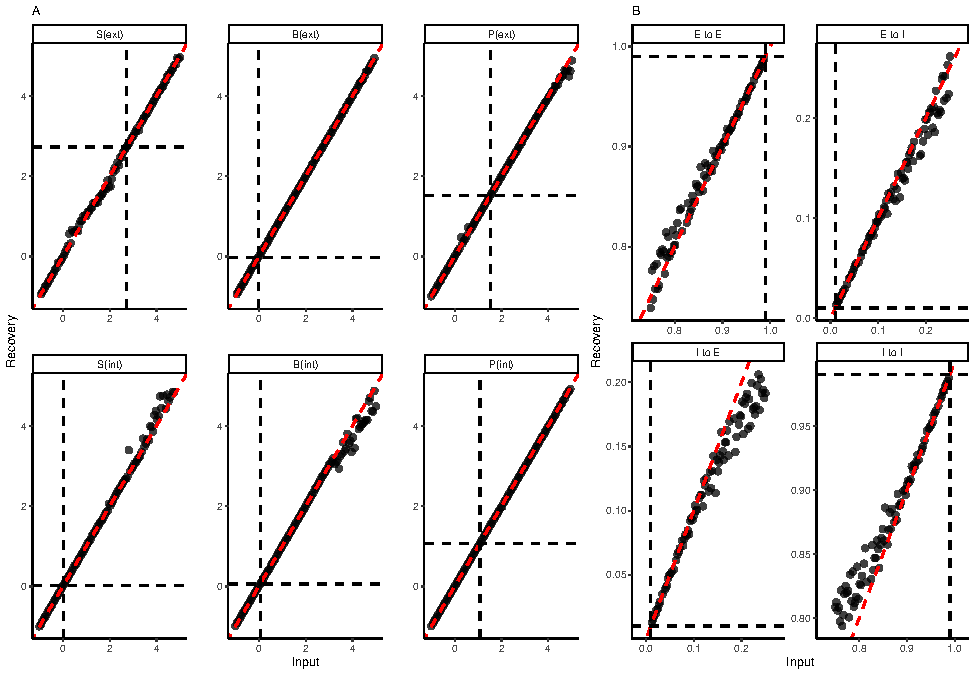
\includegraphics{modes_ketamine_scz_files/figure-latex/recovery_plot-1.pdf}
- \textbf{Supplemental Figure S1. GLM-HMM parameter recovery}

\begin{itemize}
\item
  \textbf{A. Weight recovery from simulated data: GLM weights.} The
  GLM-HMM is defined by the mode-dependent weights \(\beta_S\),
  \(\beta_B\), and \(\beta_P\). To test how well our GLM-HMM can recover
  changes in individual weights, we selected one of the six weights (3
  weights x 2 modes) and varied its value parametrically from -1 to 5.
  For each inversion, we kept all other weights at the group-level
  average obtained from the original data. For each of the six recovery
  analyses, we simulated synthetic experiences \(y_{syn}\) for n = 78400
  overlaps (number of overlaps across participants in the S-ketamine
  experiment). We then fitted a randomly initialized GLM-HMM to the
  synthetic experiences, and extracted the weights recovered from the
  synthetic experiences \(y_{syn}\). We performed each recovery for 10
  iterations, computed the average posterior weights \(\beta_S\),
  \(\beta_B\), and \(\beta_P\), and correlated them with the synthetic
  input weights. The correlation with the parametric input weights and
  the posterior weights recovered from the simulated data were close to
  1 for all weights (\(\beta_S\), \(\beta_B\), and \(\beta_P\), columns)
  and modes (external and internal, rows). Weights were recovered with
  high fidelity across a broad range of weights, and in particular at
  the group-level weights \(w_n\) obtained from the original data (black
  dotted line). The red dashed line represents the identity line (slope
  = 1, intercept = 0), indicating perfect recovery.
\item
  \textbf{B. Weight recovery from simulated data: transition matrix.} We
  repeated the above procedure for each cell of the GLM-HMM transition
  matrix. We initialized models with parametric transition probabilities
  ranging from 0.8 to 1 (on-diagonal cells, external to external,
  internal to internal) and 0 to 0.2 (off-diagonal cells, external to
  internal, internal to external). Transition probabilities were
  recovered with high fidelity across a broad range of parameters, and
  in particular at the group-level estimates obtained from the original
  data (black dotted line). The red dashed line represents the identity
  line (slope = 1, intercept = 0), indicating perfect recovery.
\end{itemize}

\subsubsection{Comment 3}\label{comment-3-1}

\textbf{I'm not entirely sure about the logic of the first two
paragraphs. While the point that reductions in precision of sensory
evidence (as may occur at the party) render us prone to making errors in
perceptual inference, this can't show why disrupted perceptual inference
plays a crucial role in schizophrenia. Rather, the party phenomenon that
they describe tentatively suggests that one of the possible mechanisms
by which the known perceptual inference disruption in schizophrenia may
occur. Apologies for the pedantry, but in essence the introductory
section seems to be saying that X may cause Y and this proves that Y is
crucial to schizophrenia. Or maybe I'm misunderstanding the point.}

We fully agree with the reviewer that the weak prediction in the party
example, which may induce erratic and surprising perceptual experiences,
are only one way perceptual inference may be altered in Scz. Our
intention was to illustrate the consequences of impaired perceptual
inference with an example, and to point to the canonical predictive
processing hypothesis of Scz, which assumes that impaired inference is
implicated in the pathophysiology of Scz.

To make our point more clear, we extended the introduction in the
following way:

\begin{itemize}
\tightlist
\item
  Imagine a dimly lit room at a crowded party, where unclear visual
  signals, indistinct sounds, and complex social interactions allow for
  multiple - and sometimes false - interpretations. In such ambiguity,
  failures of perceptual inference, the ability to contextualize sensory
  inputs with prior knowledge about the world, can lead to profound
  departures from reality: Faces obscured in shadow may appear
  distorted, random noise could be perceived as a whisper, and friendly
  smiles might seem derogatory. According to the canonical predictive
  processing hypothesis\textsuperscript{1}, a disruption of perceptual
  inference is likely to play a crucial role in schizophrenia (Scz), a
  severe mental disorder characterized by psychotic symptoms such as
  delusions and hallucinations\textsuperscript{1--3}. People with Scz
  may fail to apply prior knowledge to the interpretation of ambiguous
  sensory signals, causing erratic inferences that lead to hallucinatory
  experiences and delusional beliefs\textsuperscript{1}.
\end{itemize}

\subsubsection{Comment 4}\label{comment-4-1}

\textbf{The assertion that NMDA receptors block midbrain dopamine seems
to be a great simplification of the findings from the reference that
they cite to support this statement. The study cited examined
amphetamine-induced DA release in a NMDAR hypofunction model and the
findings were more complex and do not, in my view, support this simple
statement.}

We apologize for the imprecision in referencing what is known about the
role of NMDARs in dopamine. In response to Comment 1 of Reviewer 1, we
have rephrased the role of NMDARs in perceptual inference.

\begin{itemize}
\tightlist
\item
  (\ldots) Physiologically, precision corresponds to the postsynaptic
  gain or excitability of neuronal populations that report prediction
  errors, commonly mediated by NMDA receptor
  function\textsuperscript{8--11}.
\end{itemize}

In addition, we now provide a more nuanced description of the additional
pathways through which NMDARs may impact perceptual inference:

\begin{itemize}
\tightlist
\item
  Beyond predictive processing theory, several lines of evidence point
  to NMDAR hypofunction as a key factor in the pathophysiology of
  psychosis\textsuperscript{12}. NMDAR antibodies\textsuperscript{13}
  and antagonists such as ketamine\textsuperscript{14} mimic the
  symptoms of Scz, which is itself associated with a reduction of NMDAR
  density in the prefrontal cortex\textsuperscript{15}. In addition to
  their role in controlling the excitability of prediction error
  neurons\textsuperscript{8--11} and their general function for
  maintaining the cortical excitation-inhibition
  balance\textsuperscript{16}, NMDARs play a critical role in cortical
  feedback\textsuperscript{17}, support synaptic short-term
  plasticity\textsuperscript{18}, and interact with neuromodulators such
  as dopamine and serotonin via GABAergic
  interneurons\textsuperscript{19}. While these NMDAR-dependent
  mechanisms are likely critical for perceptual inference, it is yet to
  be determined how NMDAR hypofunction may cause the symptoms of Scz.
\end{itemize}

\subsubsection{Comment 5}\label{comment-5-1}

\textbf{I was unsure about the argument that was advanced in lines 32 to
43 in the introductory section: the idea that hallucinations that occur
as discrete events with an onset and offset separated by seconds to
minutes is fine but the cited studies (refs 12 and 13) used an
experience sampling approach that really can't say much about these the
period of these fluctuations and I'm therefore not clear on how the
current authors make the assertion that ``spontaneous fluctuations over
time \ldots{} occur at a timescale compatible with the duration of
individual psychotic experiences''.}

We fully agree, and apologize for the imprecision. We believe that it is
general clinical knowledge that psychotic experiences are discrete
events with an on- and offset, especially in early psychosis. To our
knowledge, precise measurements of the duration of individual delusional
and hallucinatory experiences are still lacking. We agree that the
experience-sampling papers we cited in the previous version do not speak
to the duration of individual hallucination\textsuperscript{71,72}. They
do suggest, however, that there are considerable fluctuations in
psychotic symptoms over time. Real-time symptom capture, which may be
more adept at characterizing the temporal duration of individual
psychotic experiences, suggests that hallucinations can be brief enough
for patients to report their start and end during an experimental
session\textsuperscript{20--22}.

In light of these uncertainties, we have now to refer to temporal
fluctuations in the experience of hallucinations in the introduction,
without making a strong statement about their expected duration, and
stress that temporal fluctuations of any sort (i.e., irrespective of
their precise duration) challenge models that assume a constant change
in perceptual inference:

\begin{itemize}
\tightlist
\item
  The second unresolved question concerns the temporal dynamics of
  psychotic experiences, which often unfold as short-lived events
  spanning from seconds to minutes, especially at early stages of Scz.
  The transient nature of psychotic experiences\textsuperscript{20--22}
  challenges models that assume a constant disruption of perceptual
  inference\textsuperscript{1--3}. A solution to this problem is
  suggested by the recent observation that perceptual inference is
  subject to spontaneous fluctuations over time\textsuperscript{23--25}.
\end{itemize}

In addition, we have added a paragraph to the discussion about future
experiments on the correlation between the duration of modes, and the
duration of individual psychotic experiences:

\begin{itemize}
\tightlist
\item
  (\ldots) Further insights into the relationship between neural modes
  and Scz symptoms could be obtained by correlating the temporal
  dynamics of psychotic experiences with the timing of mode alternations
  in individual patients. Future research could leverage real-time
  symptom capture and functional imaging to investigate whether shifts
  in neural modes coincide with the onset and offset of psychotic
  symptoms. This approach may illuminate the dynamic mechanisms that
  drive these experiences, offering a deeper understanding of the neural
  processes involved in psychosis.
\end{itemize}

\subsubsection{Comment 6}\label{comment-6-1}

\textbf{Lines 219-221 in the methods section -- the authors should check
the description of finger placement as there may be a mix up between
left and right.}

Thanks a lot for pointing this out, we apologize for the mix up. Indeed,
keys d and f were for the left hand, and k and j were for the right
hand. We corrected the text accordingly:

\begin{itemize}
\tightlist
\item
  (\ldots) (right middle-finger on k: rotation of the front-surface to
  the right at high confidence; right index-finger on j: rotation of the
  front-surface to the right at low confidence; left middle-finger on s:
  rotation of the front-surface to the left at high confidence; left
  index-finger on d: rotation of the front-surface to the left at low
  confidence; thumb on space bar: unclear direction of rotation).
\end{itemize}

\subsection{Referee: 3}\label{referee-3}

\textbf{In this study, Weilnhammer et al.~investigate if and how NMDA
hypofunction relates to perceptual decision-making and psychosis in
schizophrenia. By fitting a GLM-HMM model to perceptual reports in a
bistable perception paradigm, they identify two modes of perceptual
inference differing in terms of the influence of prior expectations --
external (weak prior) and internal (strong prior). They find that
S-ketamine increases the fraction of time healthy participants spend in
the external mode. They find a similar tendency in patients with
schizophrenia and conclude that NMDA hypofunction might cause psychosis
by shifting the dynamic balance between the two modes of perception.}

\textbf{The study design and statistical modeling are sound and novel,
and the effects of S-ketamine are very interesting. But the link to
psychosis (vs.~general cognitive factors and trait-like effects in
schizophrenia) is somewhat tenuous due to several assumptions that are
not yet supported by the data.}

\subsubsection{Comment 1}\label{comment-1-2}

\textbf{The abstract begins with a rather strong claim: ``Perception is
known to alternate between an external mode, driven by sensory inputs,
and an internal mode, shaped by prior knowledge about the world''. While
data-driven methods like GLM-HMM are increasingly being applied to
identify different modes of behavior, to my knowledge it is not
established that they correspond to modes of perceptual processing. The
interpretation of the HMM modes is necessarily limited by the hypotheses
embodied by the GLM. The GLM here is constrained to arbitrate between
prior and likelihood, and therefore not designed to falsify alternative
hypotheses pertaining to changes in task engagement, or other downstream
decision variables.}

We would like to thank the reviewer for this very insightful comment. We
agree that the statement in the previous version is too strong a claim
and have rephrased the absract accordingly (see below). If we understand
correctly, the above comments asks two questions: (i) what is the
evidence that external and internal modes are modes of perception, as
opposed to modes of behavior?; and (ii), what are the hypotheses
embodied by the GLM-HMM proposed here?

(i): GLM-HMMs are typically fitted to behavioral responses during
trial-based 2AFC decision-making experiments\textsuperscript{25,56,68}.
Some authors have labeled the states identified by the GLM-HMM as
\emph{engaged} (high stimulus-weight, low history weight) and
\emph{disengaged} (low stimulus weight, high history
weight)\textsuperscript{25,68}. This interpretation suggests that the
states identified by the GLM-HMM may be behavioral.

However, there is also recent evidence from 2AFC decision-making
suggesting that the GLM-HMM states have a perceptual quality: When
humans detect gratings in white noise, false alarm trials are more
likely after trials in which people experienced a high-contrast grating.
Moreover, false alarm trials are associated with increased power at the
orientation and spatial frequency of the preceding grating, indicating
that detection unfolds within a predictive perceptual
template\textsuperscript{37,56}. If false alarms were purely behavioral,
one would expect no correlation between orientation and power at the
spatial frequency of the target grating\textsuperscript{69}. Recent work
shows that predictive perceptual templates are particularly strong in
the internal mode\textsuperscript{56}, supporting the hypothesis that
the internal mode is indeed predictive and
perceptual\textsuperscript{56}. Moreover, an analysis that identified
external and internal modes in human 2AFC
decision-making\textsuperscript{73} based on the autocorrelation of
stimulus-congruent and history-congruent responses suggested that
confidence has a quadratic relationship with mode\textsuperscript{26}.
The observation that confidence is high for strong biases toward both
external and internal mode\textsuperscript{26} speaks against the idea
that internal mode processing can be reduced completely to disengaged
behavior.

However, we acknowledge that more data are needed to better understand
the level at which external and internal mode operate. Promising avenues
for future research could be no-report paradigms and comparisons between
neural activity during external and internal mode in low-level visual
areas.

We have rephrased the abstract as follows:

\begin{itemize}
\tightlist
\item
  Perception integrates external sensory signals with internal
  predictions that reflect prior knowledge about the world. Previous
  research suggests that this integration is governed by slow
  alternations between an external mode, driven by sensory signals, and
  an internal mode, shaped by prior knowledge. Using a double-blind,
  placebo-controlled, cross-over experiment in healthy human
  participants, we investigated the effects of the N-Methyl-D-aspartate
  receptor (NMDAR) antagonist S-ketamine on the balance between external
  and internal modes. We found that S-ketamine causes a shift of
  perception toward the external mode. A case-control study revealed
  that individuals with paranoid Scz, a disorder repeatedly associated
  with NMDAR hypofunction, spend more time in the external mode. This
  NMDAR-dependent increase in the external mode suggests that the
  symptoms of schizophrenia are caused by recurring dissociations of
  perception from prior knowledge about the world.
\end{itemize}

We have also added a paragraph to the Discussion:

\begin{itemize}
\item
  External and internal modes reflect GLM-HMM states informed by
  behavioral responses during psychophysical experiments. If mode
  alternations are linked to perceptual inference and its alteration in
  Scz, then external and internal modes should capture dynamic changes
  in perception rather than merely ongoing fluctuations in task
  engagement.
\item
  Previous studies have used GLM-HMMs to identify engaged and disengaged
  behavior in mice tasked with discriminating the location of a visual
  stimulus\textsuperscript{25,68}. While this terminology may suggest
  that GLM-HMM states reflect dynamic changes in rodent behavior,
  evidence from human psychophysics indicates that external and internal
  modes may in fact reflect perceptual (as opposed to behavioral)
  states\textsuperscript{26,56}. Specifically, when humans detect
  gratings in white noise, false alarms are more likely when the noise
  contains more power at the orientation and spatial frequency of the
  preceding grating, suggesting that detection relies on a predictive
  perceptual template\textsuperscript{37,56}. If these detection events
  were purely behavioral, no correlation between false alarms and the
  noise power spectrum would be expected\textsuperscript{69}.
  Critically, recent work demonstrates that these predictive perceptual
  templates are confined to the internal mode, supporting the hypothesis
  that the internal mode is indeed predictive and
  perceptual\textsuperscript{56}. Moreover, an analysis of 66
  experiments on human two-alterantive forced-choice decision-making
  revealed a quadratic relationship of confidence with
  mode\textsuperscript{26}. The observation that confidence remains high
  for strong biases toward both external and internal
  modes\textsuperscript{26} argues against the interpretation of
  internal mode as disengaged behavior.
\item
  Despite these findings, further research is necessary to identify
  where in the cognitive hierarchy external and internal mode take
  effect. No-report paradigms and functional imaging in low-level visual
  areas could provide more definitive evidence on how external and
  internal modes modulate perception\textsuperscript{56}, and whether
  there are additional effect on cognitive processes that occur
  downstream\textsuperscript{25,68}.
\end{itemize}

(ii): The GLM-HMM used in this study predicts experiences \(y_t\) in a
GLM that is defined by the stimulus \(\beta_S \times s_t\), the
preceding experience \(\beta_P \times y_{t-1}\), and the constant bias
\(\beta_B \times b\). The HMM component of the model identified two
states that differ with respect to the weights on any combination of the
predictors. We chose the GLM-HMM to test whether the computational
mechanism of Scz (an imbalance between internal predictions and external
sensory data, according to the prevailing hypothesis\textsuperscript{1})
is dynamic. This hypothesis is represented by a change in
\(\Delta{S-P}\) (high \(\beta_S\) and low \(\beta_P\) in external mode;
low \(\beta_S\) and high \(\beta_P\) in internal mode). However, beyond
our primary hypothesis, the GLM-HMM can in principle embody dynamic
changes in any combination of weights. Alternative outcomes to external
versus internal modes are therefore states that differ with respect to
bias (state 1: high \(\beta_B\) for strong bias, state 2: low
\(\beta_B\) for weak bias) and randomness of predictability of
perception (state 1: high \(\beta_S\) and high \(\beta_P\) for low
choice randomness; state 2: low \(\beta_S\) and low \(\beta_P\) for high
choices randomness).

In the S-ketamine experiment, \(\beta_B\), the weight associated with
the constant response bias \(b\) toward rightward rotation, was not
different from zero (\(\beta_B\) = \(0.04\) ± \(0.11\), T(\(98.36\)) =
\(0.31\), p = \(1\)). We found no effect of drug (\(-0.11\) ± \(0.14\),
T(\(81\)) = \(-0.74\), p = \(1\)) or mode (\(-0.02\) ± \(0.14\),
T(\(81\)) = \(-0.12\), p = \(1\)) on the bias weight \(\beta_B\).
\(\beta_P\), the weight associated with the previous percept \(y_{t-1}\)
was not modulated by S-ketamine (\(-0.22\) ± \(0.26\), T(\(81\)) =
\(-0.87\), p = \(1\)) or mode (\(-0.75\) ± \(0.26\), T(\(81\)) =
\(-2.92\), p = \(0.29\)). There was no significant interaction between
drug and mode with respect to \(\beta_P\) (\(0.35\) ± \(0.36\),
T(\(81\)) = \(0.97\), p = \(1\)). The balance
\(\Delta_{S-P} = \beta_S - \beta_p\) between external inputs and
internal predictions was determined by mode (\(2.8\) ± \(0.29\),
T(\(81\)) = \(9.5\), p = \(\ensuremath{5.22\times 10^{-13}}\)), with no
significant effect of S-ketamine (\(0.03\) ± \(0.29\), T(\(81\)) =
\(0.1\), p = \(1\)) and no interaction (\(0.14\) ± \(0.42\), T(\(81\)) =
\(0.34\), p = \(1\)).

In the case-control study, \(\beta_B\), the weight associated with the
constant response bias \(b\) toward rightward rotation, was not
different from zero (\(0.05\) ± \(0.18\),
T(\(\ensuremath{1.62\times 10^{-8}}\)) = \(0.29\), p = \(1\)). We found
no effect of group (\(-0.09\) ± \(0.25\),
T(\(\ensuremath{1.62\times 10^{-8}}\)) = \(-0.37\), p = \(1\)). There
was a trend for a positive effect of internal mode (\(0.6\) ± \(0.24\),
T(\(88\)) = \(2.47\), p = \(0.06\)) on the bias weight \(\beta_B\).
\(\beta_P\), the weight associated with the previous percept
\(y_{t-1}\), was reduced in internal mode (\(-0.75\) ± \(0.26\),
T(\(88\)) = \(-2.92\), p = \(0.02\)), but not modulated by group
(\(0.17\) ± \(0.32\), T(\(\ensuremath{9.88\times 10^{-10}}\)) =
\(0.54\), p = \(1\)). There was no significant interaction between group
and mode with respect to \(\beta_P\) (\(0.11\) ± \(0.36\), T(\(88\)) =
\(0.3\), p = \(1\)). The balance \(\Delta_{S-P} = \beta_S - \beta_p\)
between external inputs and internal predictions was determined by mode
(\(1.44\) ± \(0.33\), T(\(81\)) = \(9.5\), p =
\(\ensuremath{3.39\times 10^{-4}}\)), with no significant effect of
group (\(0.28\) ± \(0.54\), T(\(87.97\)) = \(0.52\), p = \(1\)) and no
interaction (\(0.36\) ± \(0.47\), T(\(44\)) = \(0.76\), p = \(1\)).

The above data, which are summarized Supplemental Figure S3 and 4,
therefore speak in favor of the modes hypothesis (high \(\beta_S\) and
low \(\beta_P\) in external mode; low \(\beta_S\) and high \(\beta_P\)
in internal mode), and against the hypothesis that the dominant state
changes are driven by the dynamics of bias or randomness. We have added
a description of the state changes compatible with the GLM-HMM in the
Methods and Supplemental Figures S2-3.

\begin{itemize}
\item
  Methods: (\ldots) The GLM-HMM used in this study predicts experiences
  \(y_t\) in a GLM defined by the stimulus \(s_t\), the preceding
  experience \(y_{t-1}\), and a constant bias \(b\). The HMM component
  of the model identifies alternations between two states that differ
  with respect to the weights of any combination of \(s_t\),
  \(y_{t-1}\), and \(b\). We used the GLM-HMM to test our primary
  hypothesis that ketamine and Scz alter the balance between two states
  that differ with respect to \(\Delta_{S-P} = \beta_S - \beta_P\) (high
  \(\Delta_{S-P}\) in external mode, low \(\Delta_{S-P}\) in internal
  mode: hypothesis H2). However, the GLM-HMM can, in principle, embody
  dynamic changes in any combination of \(\beta_S\), \(\beta_B\), and
  \(\beta_P\). Alternative outcomes to external versus internal modes
  are states that differ with respect to bias (state 1: high
  \(\beta_B\); state 2: low \(\beta_B\); hypothesis H3) and randomness
  (state 1: high \(\beta_S\) and \(\beta_P\); state 2: low \(\beta_S\)
  and \(\beta_P\): no difference in \(\Delta_{S-P}\) between modes:
  hypothesis H4).
\item
  Supplemental Figure S3: (\ldots) These posterior GLM-HMM weights argue
  against the alternative hypotheses that the primary effect of
  S-ketamine is related to changes in dynamics of bias (state 1: high
  \(\beta_B\); state 2: low \(\beta_B\); hypothesis H3) or the
  randomness of experience (state 1: high \(\beta_S\) and \(\beta_P\);
  state 2: low \(\beta_S\) and \(\beta_P\) with no difference in
  \(\Delta_{S-P}\) between modes: hypothesis H4).
\item
  Supplemental Figure S4: (\ldots) These posterior GLM-HMM weights argue
  against the alternative hypotheses that the primary effect of Scz is
  related to changes in dynamics of bias (state 1: high \(\beta_B\);
  state 2: low \(\beta_B\); hypothesis H3) or the randomness of
  experience (state 1: high \(\beta_S\) and \(\beta_P\); state 2: low
  \(\beta_S\) and \(\beta_P\) with no difference in \(\Delta_{S-P}\)
  between modes: hypothesis H4).
\end{itemize}

\subsubsection{Comment 2}\label{comment-2-2}

\textbf{Both patients and healthy participants on S-ketamine reportedly
spend more time in the external mode. The authors take this to imply an
alteration in perceptual processing without ruling out alternative
explanations. First, since model parameters are fit to participants'
choices, the results may stem from alterations in choice persistence.
Specifically, spending more time in the external mode likely results in
more response switches and therefore decreased choice persistence. This
confound needs to be addressed, if possible, by analyzing the data by
including confidence reports which may help decouple stimulus-history
and choice-history effects -- perhaps the authors can make model-based
predictions they can test in the data using the confidence data to speak
to this point.}

We would like to thank the reviewer for pointing out this important
point. Our paradigm relies on explicit perceptual choices that we take
as indicators of the participants' perceptual experience of the
stimulus. Participants were instructed to report changes in conscious
experience (often referred to as switches in bistable perception). For
structure-from-motion stimuli like those used in this study, switches
are most likely to occur at overlapping configurations of the
stimulus\textsuperscript{28,33,41,42} (i.e., when the bands that compose
the stimulus overlap, see Supplemental Video S1-2). This effect, which
was replicated in the S-ketamine experiment (Supplemental Figure S2A)
and the case-control study (Supplemental Figure S5A), allowed us to
discretize the behavioral data and label each overlap with an experience
\(y_t\), the stimulus \(s_t\), and the preceding experience \(y_{t-1}\)
(see Methods and Figure 1C). However, participants did not report their
choice at every overlap, but only when they experienced a change in the
direction of rotation. RTs in our study are defined by the time at which
a participant indicates a change in conscious experience, relative the
time at which the last preceding overlap
occurred\textsuperscript{28,33,42}.

Our paradigm therefore differs from classic 2AFC decision-making
experiments, where explicit choices are available for every trial. Slow
alternations between external and internal modes have been identified as
a general phenomenon in 2AFC perceptual decision-making, occurring
across a wide variety of tasks and modalities\textsuperscript{26}. Prior
work has shown that stabilizing internal predictions, which are
particularly strong in the internal mode, are better explained by the
effects of choice history, as opposed to the effects of stimulus history
(S1 Text\textsuperscript{26}).

Since our paradigm does not require choices at every overlap, choice
persistence is unlikely to be the primary driver of what we identified
as internal mode. However, we fully agree that it is important to
provide additional justification for the interpretation that external
and internal modes are perceptual phenomena. We have performed three
additional analyses:

\begin{enumerate}
\def\labelenumi{(\roman{enumi})}
\tightlist
\item
  In our experiment, stabilizing internal predictions biased perception
  toward preceding overlaps (\(t-1\)), creating conflicts between the
  consciously experienced rotation direction (\(y\)) and the current
  stimulus (\(s\)). If external and internal modes are perceptual
  phenomena, perception stabilization should be driven by the sequence
  of experiences (\(y\)) rather than stimuli (\(s\)). To test this, we
  compared an experienced-based GLM-HMM, where internal predictions are
  driven by the previous perceptual experience, with a stimulus-based
  GLM-HMM, where predictions are driven by the previous stimulus.
  Consistent with prior findings\textsuperscript{26}, we observed a
  lower BIC for the experienced-based GLM-HMM in both the S-ketamine
  experiment (\(\delta_{BIC}\) = \(\ensuremath{-7.4\times 10^{3}}\)) and
  the case-control study (patients: \(\delta_{BIC}\) = \(-981.65\);
  controls: \(\delta_{BIC}\) = \(-862.91\)), indicating that our data
  were better explained by dynamic fluctuations in the balance between
  the current stimulus \(s_t\) and the previous experience \(y_{t-1}\)
  (experience history), as opposed to dynamic fluctuations in the
  balance between the current stimulus \(s_t\) and the previous stimulus
  \(s_{t-1}\) (stimulus history).
\end{enumerate}

\begin{enumerate}
\def\labelenumi{\roman{enumi})}
\setcounter{enumi}{1}
\tightlist
\item
  Our GLM-HMM generates a perceptual decision variable \(P(y_t = 1)\)
  that is defined by a weighted integration of the current external
  stimulus (\(\beta_S \times s_t\)) and the previous experience
  (\(\beta_P \times y_{t-1}\)). The weights are obtained by fitting the
  GLM-HMM to the sequence of experiences \(y\). If external and internal
  modes are perceptual phenomena, the GLM-HMM perceptual decision
  variable should not only explain the contents of experience (which the
  model is fitted to), but also predict metacognitive processes that
  occur downstream of perception, such as reports of perceptual
  confidence (which the model was not fitted to). This generates two
  testable hypotheses for the confidence reports obtained in our
  experiment:
\end{enumerate}

iia) The posterior certainty of the GLM should correlate with subjective
confidence reports. The posterior certainty can be represented by log
probability of the actual experience \(y\), given the decision variable
\(P(y_t = 1)\):

\[
C_t = y_t \cdot \log(P(y_t = 1)) + (1 - y_t) \cdot \log(1 - P(y_t = 1)) 
\]

Importantly, any correlation between the posterior certainty \(C_t\) and
confidence provides an independent validation of our GLM-HMM, since the
model was not fitted to the trial-wise confidence ratings. Indeed, the
posterior certainty extracted from the two-state GLM-HMM predicted
trial-wise confidence reports (\(0.29\) ± \(0.02\), z = \(15.4\), p =
\(\ensuremath{1.54\times 10^{-53}}\)). Importantly, there was no
interaction with mode (\(-0.07\) ± \(0.07\), z = \(-1.03\), p =
\(0.3\)), confirming that the positive correlation between posterior
certainty and confidence was present in both external and internal
modes. The posterior certainty extracted from the two-state GLM-HMM was
better at explaining confidence than the one-state control GLM
(\(\delta_{BIC}\) = -280.69), and the one-state stimulus GLM
(\(\delta_{BIC}\) = -445.13). The superiority of the two-state GLM over
the control GLMs in predicting the out-of-training confidence reports
validates that perception is indeed modulated by slow alternations
between external and internal modes.

iib) If external and internal modes are perceptual phenomena, internal
mode should be associated with lower metacognitive performance (i.e.,
the degree to which confidence reports reflect perceptual accuracy).
This is because, in the internal mode, stabilizing internal predictions
have a larger effect on perception, causing subjective experiences that
are less constrained by the external input. If, by contrast, external
and internal modes occur at the level of response behavior (i.e., choice
persistence), metacognitive performance should not be affected by mode.
Indeed, in our data, accuracy was predictive of high confidence across
modes (\(1.01\) ± \(0.05\), z = \(18.7\), p =
\(\ensuremath{4.63\times 10^{-78}}\)), but to a lesser degree during the
internal mode (\(-0.61\) ± \(0.09\), z = \(-6.61\), p =
\(\ensuremath{3.94\times 10^{-11}}\)). In line with this, metacognitive
sensitivity, as measured by meta-d'\textsuperscript{43}, was
significantly lower in the internal mode (\(-1.6\) ± \(0.45\), T(\(50\))
= \(-3.55\), p = \(\ensuremath{3.41\times 10^{-3}}\)).

In light of these results, we have made the following changes to the
manuscript:

We have added the above analyses to the methods:

\begin{itemize}
\item
  \textbf{Stimulus- versus experienced-based GLM-HMM.} In our
  experiment, stabilizing internal predictions bias perception toward
  preceding overlaps (\(t-1\)), causing conflicts between the direction
  of rotation that is consciously experienced (\(y\)) and the stimuli
  \(s\) presented at the current overlap \(t\). If external and internal
  modes are perceptual in nature, then the stabilization of perception
  should be driven by the sequence of perceptual experiences \(y\), as
  opposed to the sequence of sensory signals \(s\) (hypothesis H5). To
  test this hypothesis, we compared our \emph{experienced-based}
  GLM-HMM, in which the stabilizing internal predictions are driven by
  the participants' perceptual experience at the preceding overlap, with
  an alternative \emph{stimulus-based} GLM, in which the stabilizing
  internal predictions are driven by the stimulus presented at the
  preceding overlap.
\item
  \textbf{External validation of the GLM-HMM.} The GLM-HMM generates a
  perceptual decision variable \(P(y_t = 1)\) that is defined by a
  weighted integration of the external stimulus
  (\(\beta_S \times s_t\)), the previous experience
  (\(\beta_P \times y_{t-1}\)), and a constant bias
  (\(\beta_P \times 1\)). The weights are obtained by fitting the
  GLM-HMM to the sequence of experiences \(y\), irrespective of whether
  the experience \(y\) was made at high or low confidence. This allowed
  us to test whether the predictions of the two-state GLM-HMM would
  generalize to metacognitive reports on perception. Importantly, the
  source of confidence differs between the modes: During the external
  mode, confidence should depend predominantly on the SAR of the
  stimulus. Conversely, during the internal mode, confidence should be
  driven more by the congruency of perception with previous experiences,
  and less by the external input. To validate our model, we tested
  whether the perceptual decision variable \(P(y_t = 1)\) predicted not
  only the binary contents of experience \(y_t\) (which the GLM-HMM was
  fitted to), but also perceptual confidence \(c_t\) (which the GLM-HMM
  was not fitted to). To do so, we correlated \(c_t\) (as reported by
  the participants) with the posterior certainty \(C_t\) (as provided by
  the GLM-HMM) at each overlap. The posterior certainty \(C_t\) is given
  by log probability of the actual experience \(y\), given the decision
  variable \(P(y_t = 1)\):
\end{itemize}

\[
C_t = y_t \cdot \log(P(y_t = 1)) + (1 - y_t) \cdot \log(1 - P(y_t = 1))  
\]

\begin{itemize}
\tightlist
\item
  To assess differences in metacognitive performance, we correlated
  perceptual confidence with perceptual accuracy. We computed meta-d', a
  measure of metacognitive sensitivity that indicates how well
  confidence ratings predict perceptual accuracy\textsuperscript{43}.
\end{itemize}

We have added the following analyses to the results:

\begin{itemize}
\item
  Our results suggest that healthy participants under S-ketamine and Scz
  patients spend more time in the external mode. As a dynamic mechanism
  for psychotic experiences, alternations between external and internal
  mode should have an effect at the level of perception. This means that
  between-mode alternations should modulate a perceptual decision
  variable that determines not only what is consciously experienced, but
  also how the contents of perception are evaluated by downstream
  cognition. The hypothesis that external and internal modes are
  perceptual phenomena needs to be contrasted against alternative
  scenarios in which external and internal modes are driven primarily by
  fluctuations in arousal, high-level cognition, or executive function.
\item
  To address these alternative accounts, we first performed additional
  tests to support our claim that external and internal mode operate at
  the level of perception. External and internal modes are states of a
  GLM-HMM that integrates the external stimulus \(s_t\) with the
  previous experience \(y_{t-1}\) into a perceptual decision variable
  \(P(y_t = 1)\). The parameters of the GLM-HMM are optimized to predict
  the sequence of perceptual experiences \(y_t\) from \(P(y_t = 1)\). If
  external and internal modes are perceptual phenomena, then the
  stabilization of perception should be driven by the sequence of
  experiences \(y_t\), as opposed to the sequence of stimuli \(s_t\). To
  test this hypothesis, we compared our \emph{experienced-based}
  GLM-HMM, in which the stabilizing internal predictions are driven by
  the participants' perceptual experience at the preceding overlap, with
  an alternative \emph{stimulus-based} GLM, in which the stabilizing
  internal predictions are driven by the stimulus presented at the
  preceding overlap. Bayesian model comparison indicated that the
  experienced-based GLM-HMM was better at explaining our data than a
  stimulus-based GLM-HMM in the S-ketamine experiment (\(\delta_{BIC}\)
  = \(\ensuremath{-7.4\times 10^{3}}\)) and the case-control study
  (patients: \(\delta_{BIC}\) = \(-981.65\); controls: \(\delta_{BIC}\)
  = \(-862.91\)).
\item
  Moreover, if external and internal modes are perceptual phenomena,
  then the decision variable \(P(y_t = 1)\) should not only determine
  the contents of perception, but also metacognitive processes that
  depend on them. To assess this prediction, we tested whether the
  posterior certainty \(C_t\) at which the GLM-HMM predicted the content
  of perception, i.e., the log probability of the experience \(y_t\)
  given the decision variable \(P(y_t = 1)\)
  (\(C_t = y_t \cdot \log(P(y_t = 1)) + (1 - y_t) \cdot \log(1 - P(y_t = 1))\)),
  would correlate with the confidence reports \(c_t\) in the S-ketamine
  experiment. This test is a powerful validation of our approach, since
  the GLM-HMM was only fitted to binary perceptual states \(y_t\), and
  not to the confidence \(c_t\) at which they were reported. Indeed,
  \(C_t\) predicted the confidence reports \(c_t\)(\(\beta\) = \(0.29\)
  ± \(0.02\), z = \(15.4\), p = \(\ensuremath{1.54\times 10^{-53}}\))
  without an interaction with mode (\(\beta\) = \(-0.07\) ± \(0.07\), z
  = \(-1.03\), p = \(0.3\)), confirming that the positive correlation
  between posterior certainty and confidence was present in both
  external and internal modes. \(C_t\) extracted from the two-state
  GLM-HMM was better at explaining confidence than the one-state control
  GLM (\(\delta_{BIC}\) = -280.69), and the one-state stimulus GLM
  (\(\delta_{BIC}\) = -445.13).
\item
  As a consequence, internal mode should be associated with lower
  metacognitive performance (i.e., the degree to which confidence
  correlates accuracy), since stabilizing internal predictions have a
  larger effect on perception in the internal mode, and cause
  experiences \(y_t\) to be less constrained by the external input
  \(s_t\). Indeed, accuracy was predictive of high confidence (\(\beta\)
  = \(1.01\) ± \(0.05\), z = \(18.7\), p =
  \(\ensuremath{4.63\times 10^{-78}}\)), but to a lesser degree during
  the internal mode (\(\beta\) = \(-0.61\) ± \(0.09\), z = \(-6.61\), p
  = \(\ensuremath{3.94\times 10^{-11}}\)). In line with this,
  metacognitive sensitivity, as measured by meta-d', was significantly
  lower in the internal mode (\(\beta\) = \(-1.6\) ± \(0.45\), T(\(50\))
  = \(-3.55\), p = \(\ensuremath{3.41\times 10^{-3}}\)). Together, these
  findings support the hypothesis that external and internal modes
  modulate a low-level decision variable \(P(y_t = 1)\) that determines
  the content of perception and their metacognitive evaluation.
\end{itemize}

We briefly refer to these results in the discussion:

\begin{itemize}
\tightlist
\item
  Beyond predicting the contents of perception, the GLM-HMM is capable
  of predicting confidence, a cognitive variable to which the model was
  not fitted. In line with previous results\textsuperscript{26}, this
  observation suggests that external and internal modes modulate a
  perceptual decision variable that influences not only what is
  consciously experienced, but also downstream processes such as
  metacognition.
\end{itemize}

\subsubsection{Comment 3}\label{comment-3-2}

\textbf{Second, S-ketamine clearly affects wakefulness and nervousness
as shown in figure S5. These are very useful findings, but again it is
possible that these internal states alter the level of motor or general
task engagement, and in turn, the model parameters. Can the authors
demonstrate that S-ketamine induced changes in the model parameters are
conditionally independent of its effect on these internal states?}

We would like to thank the reviewer for pointing out this important
caveat. We addressed this concern in two steps. We show that over and
above dynamic changes in wakefulness (Q1), subjective intoxication (Q2),
and nervousness (Q3), S-ketamine has an effect on mode (i), and mode has
an effect on how perception integrates internal predictions with
external inputs (ii).

(i): Our results show that S-ketamine \emph{increased} external mode,
\emph{reduced} wakefulness (Q1), and \emph{increased} feelings of
intoxication (Q2) as well as nervousness (Q3). If changes in these
states were to explain the effects of s-ketamine on mode fluctuations
through changes in general task engagement, one would expect a
\emph{decrease} rather than an \emph{increase} in external mode.
However, to make sure that the effect of S-ketamine is not driven by
drug-related effects on Q1, Q2, and Q3, we added these time-resolved
subjective reports to the random effects structure of the mixed effects
model that tests the effect of S-ketamine on the balance between modes.
The effect of mode remained highly significant when controlling for
these variables (p \textless{} \(\ensuremath{7.89\times 10^{-10}}\)).

(ii): Our analyses indicate that S-ketamine has an effect on perception
via its effect on mode. We therefore performed additional anlayses to
rule out that the effects of mode on the model parameters are driven
dynamic changes in Q1-3. To this end, we tested the effect of mode on
\(\Delta_{S-P} = \beta_S - \beta_P\), i.e., the difference in the weight
associated with the stimulus (\(\beta_S\)) and the weight associated
with the previous percept (\(\beta_S\)), while controlling for our
time-resolved measures of Q1-Q3. In line with the hypothesis that the
mode-dependent changes in \(\Delta_{S-P}\) are conditionally independent
of wakefulness, subjective intoxication and nervousness, we observed a
main effect of mode on \(\Delta_{S-P}\) (p =
\(\ensuremath{1.29\times 10^{-5}}\)). We also found a significant
\emph{negative} effect of subjective intoxication on \(\Delta_{S-P}\).
This effect does not explain the effects of S-ketamine, since S-ketamine
\emph{increased} subjective intoxikation (Supplemental Figure S5) and,
via its effect on mode, \(\Delta_{S-P}\). There were no additional main
effects of Q1 or Q3, nor any interactions of Q1-3 with mode.

We have added these analyses to the result section:

\begin{itemize}
\tightlist
\item
  Second, we asked whether fluctuations in global brain states can
  provide an alternative explanation for external and internal modes.
  One could assume that mode alternations could in fact reflect dynamic
  states of arousal, with high arousal and engaged behavior
  corresponding to the external mode, and low arousal and disengaged
  behavior corresponding to the internal mode. Our time-resolved
  assessment of internal states revealed reduced wakefulness (Q1) under
  S-ketamine (Supplemental Figure S6). This observation is clearly
  incompatible with the hypothesis that changes in the dynamics of mode
  are driven by low arousal under S-ketamine, since NMDAR antagonism
  increased the prevalence of the external mode, improving behavioral
  performance in the artificial setting of our experiment. When
  controlling for dynamic changes in wakefulness (Q1), subjective
  intoxication (Q2) and nervousness (Q3), the effect of S-ketamine on
  mode (p = \(\ensuremath{8.21\times 10^{-67}}\)) and the effect of mode
  on \(\Delta_{S-P}\) remained significant (p =
  \(\ensuremath{1.29\times 10^{-5}}\)). We observed no additional
  effects of or interactions with Q1-3 that could explain the observed
  relations between S-ketamine, mode, and \(\Delta_{S-P}\). Despite its
  positive effect on perceptual accuracy, external mode was associated
  with higher levels of dissociation in the S-ketamine experiment as
  measured by the
  \emph{Clinician-Administered-Dissociative-States-Scale}\textsuperscript{34}
  (CADSS, \(\beta\) = \(1.05\) ± \(0.54\), T(\(208.05\)) = \(1.95\), p =
  \(0.05\), Supplemental Figure S6B).
\end{itemize}

\subsubsection{Comment 4}\label{comment-4-2}

\textbf{Even if the effects of S-ketamine are perceptual, it is unclear
whether it reflects the pathophysiology of psychotic symptoms. If I
understood correctly, on average, S-ketamine improves (!) behavioral
accuracy by making participants more responsive to actual changes in
motion structure. It is not immediately obvious that this captures the
phenomenology of psychosis since the latter typically results in seeing
phantom structures in stimuli. Although both individuals on S-ketamine
and patients with schizophrenia spend more time in the external mode in
this task, this similarity could stem from factors unrelated to
psychosis. Both ketamine and schizophrenia as a whole (vs.~severity of
psychotic symptoms specifically) are known to be associated with general
cognitive dysfunction, which are likely to produce general alterations
in cognitive performance (vs.~specific psychosis-related alterations in
perceptual inference) explaining observed behaviors. Therefore, it is
especially jarring that the absence of any correlation between mode
transition dynamics and psychosis proneness/severity measures is given
short shrift (line 121 and caption S5F). Does the external mode
correlate with IQ or other cognitive measures in healthy participants?
Ideally the authors should demonstrate that general cognitive impairment
or lower cognitive performance in healthy individuals does not manifest
as increased external mode and that therefore their observations cannot
be attributed to domain-general alterations. Ketamine is also known to
recapitulate negative symptoms and induce cognitive impairment, which
cannot be clearly ruled out based on these data as it stands. Similarly,
the cited papers such as the Adams paper clearly separate trait-like
alterations in schizophrenia from psychosis-related state-dependent
changes, which can manifest differently or even with opposite
phenotypes: the key question is whether what is reported here is a
general trait-like phenomenon in schizophrenia (presumably linked to
general cognitive impairment also present to some degree under ketamine)
or to psychotic states. The default would be to assume the former unless
the authors can show psychosis-severity dependence and lack of
dependence on broader cognitive impairment (e.g., attentional or
executive function impairment). Both would be interesting findings but
this distinction is key to ongoing debates.}

Thanks a lot for pointing out this important question. Regarding the
assertion that our behavioral findings to not seem to capture the
phenomenology of psychosis, we would like to point out that improved
behavioral accuracy, which is what we observed not only in healthy
subjects under s-ketamine but also in patients with Scz, is precisely
what one would expect based on the existing literature on perceptual
alterations in Scz. Prior work has indeed shown that patients with
schizoprenia are less susceptible to a number of perceptual illusions,
where prior knowledge biases perception in ways that may be adaptive in
natural environments but reduce perceptual accuracy in experimental
settings\textsuperscript{59,60}.

However, we fully agree with the reviexwer that, based on our data, we
cannot make a strong claim about whether the balance of external and
internal mode is a trait, or is (also) related to the state of
psychosis. Our experiments maximized intra-subject power, and were not
designed to detect inter-individual differences, for which much larger
samples would be required. Likewise, we did not monitor psychotic
experience in real time during our experiments, which were unlikely to
occur given the dose of S-ketamine in the S-ketamine intervention study,
and the clinical status of the patients in the case-control study. In
addition to recent work on the role of mode for false
alarms\textsuperscript{56}, we believe that more research is needed to
determine whether the balance between modes is a mere trait, potentially
linked to aspects of cognition, or whether either of the modes (or their
interaction) has a particular role to play for individual psychotic
experiences.

We have modified the discussion accordingly:

\begin{itemize}
\item
  (\ldots) These findings bear similarity with prior work on perceptual
  illusions, where prior knowledge biases perception in ways that may be
  adaptive in natural environments but reduce perceptual accuracy in
  experimental settings\textsuperscript{59,60}: Weak predictions may
  therefore explain why people with Scz are, for example, less
  susceptible to the hollow-mask illusion, where knowledge about faces
  is thought to induce the experience of a convex face on the concave
  surface of a human mask\textsuperscript{39}, the Ebbinghaus illusion,
  where larger circles make a smaller central circle appear
  bigger\textsuperscript{40}, or the force-matching illusion, where
  humans apply less force when matching an externally applied force with
  their own\textsuperscript{38}.
\item
  (\ldots) In the present data, we did not find a correlation of the
  balance between external and internal mode with either global
  psychosis proneness or the clinical severity of Scz (Supplemental
  Figure S6). Our study was optimized for within-participant power and
  not designed to detect correlations between inter-individual
  differences in Scz-related traits and the balance between external and
  internal modes. One key question moving forward is whether the shift
  toward external mode represents a general trait-like phenomenon in
  Scz, potentially linked to cognitive alterations that are also present
  to some degree under ketamine\textsuperscript{67}, or whether external
  and internal modes are associated with psychosis-related,
  state-dependent changes in inference. Future research could address
  these questions by correlating the balance between modes with both
  positive and negative symptoms, as well as with measures of cognitive
  performance such as IQ in larger samples. Another promising approach
  to distinguish between trait and state effects, which can manifest
  differently or even with opposite phenotypes\textsuperscript{3}, could
  involve real-time symptom tracking combined with functional imaging.
  Such analyses could help to examine whether shifts between external
  and internal modes align with the on- and offset of individual
  psychotic experiences\textsuperscript{56}, both at the behavioral
  level and in terms of their neural correlates.
\item
  Previous studies have used GLM-HMMs to identify engaged and disengaged
  behavior in mice tasked with discriminating the location of a visual
  stimulus\textsuperscript{25,68}. While this terminology may suggest
  that GLM-HMM states reflect dynamic changes in rodent behavior,
  evidence from human psychophysics indicates that external and internal
  modes may in fact reflect perceptual (as opposed to behavioral)
  states\textsuperscript{26,56}. Specifically, when humans detect
  gratings in white noise, false alarms are more likely when the noise
  contains more power at the orientation and spatial frequency of the
  preceding grating, suggesting that detection relies on a predictive
  perceptual template\textsuperscript{37,56}. If these detection events
  were purely behavioral, no correlation between false alarms and the
  noise power spectrum would be expected\textsuperscript{69}.
  Critically, recent work demonstrates that these predictive perceptual
  templates are confined to the internal mode, supporting the hypothesis
  that the internal mode is indeed predictive and
  perceptual\textsuperscript{56}. Moreover, an analysis of 66
  experiments on human 2AFC decision-making revealed a quadratic
  relationship of confidence with mode\textsuperscript{26}. The
  observation that confidence remains high for strong biases toward both
  external and internal modes\textsuperscript{26} argues against
  reducing internal mode processing to disengaged behavior.
\item
  Our present analyses of confidence and response times, as well as our
  time-resolved assessment of wakefulness, subjective intoxication, and
  nervousness, strongly support the idea that external and internal
  modes are perceptual phenomena, cannot be reduced to processes
  occurring solely at the level of task engagement, and are not mere
  reflections of fluctuations in arousal. These observations do not,
  however, rule out the possibility that external and internal modes
  have multiple and potentially independent effects on the brain,
  including influences on high-level cognition and response behavior, or
  that they are, to some degree, dependent on global brain states.
  No-report functional imaging experiments, where the content of
  experiences is decoded without overt behavioral
  signals\textsuperscript{70}, alongside pupillometry, manipulations of
  neuromodulators that regulate global brain states, or non-invasive
  brain stimulation, could help illuminate the causes and consequences
  of these modes across the cortical hierarchy. Mapping the
  neurocomputational dynamics of mode alternations will be crucial to
  testing whether adjusting the balance between modes can mitigate
  psychotic experiences and ultimately improve the lives of people
  living with Scz.
\end{itemize}

\subsubsection{Comment 5}\label{comment-5-2}

\textbf{A 2-state GLM-HMM would have 4 transition probabilities (2 stay
and 2 switch). The probability of external mode reported here is a
marginal probability that reflects the contribution of both
E-\textgreater E (stay) and I-\textgreater E (switch) transitions, and
an increase either parameter would manifest as an increase in the
external mode. It wasn't clear which of these parameters was primarily
affected by S-ketamine, and how this compares to patients in
schizophrenia. Plotting all 4 parameters of the HMM would provide a
better characterization of the changes induced by S-ketamine and how it
compares to alterations in schizophrenia.}

We have updated the Supplemental Figure S3 and S4 accordingly, referring
to EE and II as mode stay, and EI and IE as switch transitions.
S-ketamine and Scz both increase the stability of external mode at the
expense of internal mode, with no effect on the transitions between
modes. We made the following changes to the Figure legend:

\begin{itemize}
\item
  Supplemental Figure S3D. (\ldots) S-ketamine (red) increased the
  probability of external mode (\(1.01\) ± \(0.03\), z = \(30.7\), p =
  \(\ensuremath{4.26\times 10^{-206}}\)) relative to placebo (blue) by
  modulating the stability of external and internal mode (EE versus II;
  left panels; V = 264, p = 0.01), with no effect on the transition
  probabilities between modes (EI versus IE; right panels; V = 149, p =
  0.37). (\ldots)
\item
  Supplemental Figure S4D. (\ldots) Relative to controls (blue),
  patients (red) spent more time in external mode (\(0.52\) ± \(0.03\),
  z = \(16.88\), p = \(\ensuremath{1.23\times 10^{-63}}\)). This effect
  was driven by an increase in the stability of external mode at the
  expense of internal mode (EE versus II; left panels; W = 352, p =
  0.03). There was no effect of group on the transition probabilities
  between modes (EI versus IE; right panels; W = 248, p = 0.65).
\end{itemize}

The results now refer to this result:

\begin{itemize}
\tightlist
\item
  Indeed, S-ketamine did not alter the weights of the two-state GLM-HMM
  (Figure 2C), but increased the probability of external at the expense
  of internal mode (\(\beta\) = \(1.01\) ± \(0.03\), z = \(30.7\), p =
  \(\ensuremath{4.26\times 10^{-206}}\), Figure 2D) via an effect on the
  stay transitions of the HMM (external-to-external and
  internal-to-internal, Supplemental Figure S3D).
\end{itemize}

\subsubsection{Comment 6}\label{comment-6-2}

\textbf{It would be helpful to clearly define all the statistics
somewhere. While the writing is generally clear and the figures appear
to support the claims, the statistics reported in the main text are
difficult to comprehend. Here are some examples but the authors need to
check the manuscript for other examples:}

\textbf{Line 73: Importantly, S-ketamine caused perception to shift
toward st (0.45±0.08). Is 0.45 the increase in beta\_s due to
S-ketamine?}

\textbf{Line 105: S-ketamine did not alter the weights of the two-state
GLM-HMM (Figure 2C), but increased the probability of external at the
expense of internal mode (1.01 ± 0.03). What is 1.01 here? It cannot be
the change in probability.}

\textbf{Line 117: Scz patients spent more time in external mode
(0.52±0.03). Is it 0.52 seconds, minutes, or something else?}

\textbf{Line 136: healthy participants were more confident in their
choices (0.72 ± 0.07). What is 0.72?}

We apologize for the lack of clarity. The above numbers refer to the
estimate (\(\beta\)) from the mixed effects models. We now report the
mixed effects model estimates as \(\beta\) without any subscript. All
parameter estimates with subscript refer to posterior parameters
(weights) from the GLM-HMM. We have added this information to the method
section:

\begin{itemize}
\tightlist
\item
  Mixed effects models are reported with the estimate (\(\beta\) without
  subscript), followed by the T- or z-statistic for linear and logistic
  models, respectively. Please note that parameter estimates with
  subscripts refer exclusively to the GLM-HMM weights (see Computational
  modeling) associated with the external input (\(\beta_S\)), the
  constant bias (\(\beta_B\)), and the previous experience
  (\(\beta_P\)).
\end{itemize}

\subsubsection{Comment 7}\label{comment-7}

\textbf{For the benefit of the readership, I would encourage the authors
to try to put their results in the broader context of the literature on
psychosis, clearly identifying points of agreement or departure from
prior studies that examine psychosis from alternative theoretical
perspectives e.g., circular inference and strong priors (e.g., Corlett
et al.~2019; Schmack et al., 2021; Cassidy et al.~2018; Bansal et
al.~2021\ldots)}

We would like to thank the reviewer for this suggestion. Our initial
version was written in a short format. We have now included an extensive
Dicussion section, and place our findings in the broader context of
predictive processing and circular inference:

\begin{itemize}
\item
  These findings bear similarity with prior work on perceptual
  illusions, where prior knowledge biases perception in ways that may be
  adaptive in natural environments but reduce perceptual accuracy in
  experimental settings\textsuperscript{59,60}: Weak predictions may
  therefore explain why people with Scz are, for example, less
  susceptible to the hollow-mask illusion, where knowledge about faces
  is thought to induce the experience of a convex face on the concave
  surface of a human mask\textsuperscript{39}, the Ebbinghaus illusion,
  where larger circles make a smaller central circle appear
  bigger\textsuperscript{40}, or the force-matching illusion, where
  humans apply less force when matching an externally applied force with
  their own\textsuperscript{38}.
\item
  Our findings therefore align with the canonical predictive processing
  account of psychosis\textsuperscript{1--3}. According to this model,
  NMDAR hypofunction\textsuperscript{13} and Scz\textsuperscript{28} are
  associated with weak priors that cause erratic inferences in
  perception and cognition, ultimately leading to psychotic symptoms
  such as delusions and hallucinations. At the same time, they seem at
  odds with the observation that psychotic experiences, and in
  particular false alarms that serve as an experimental proxy for
  hallucinations, correlate with strong priors\textsuperscript{61--63}.
  So far, attempts to reconcile these disparate sets of findings suggest
  that priors may vary in strength depending on the phase of psychotic
  illness, with weak priors in early stages and strong priors in later
  stages, or depending on their position within the cognitive hierarchy,
  with weak priors at the perceptual level and strong priors at the
  cognitive level\textsuperscript{1}. As an alternative to predictive
  processing, circular inference accounts of Scz posit that psychotic
  symptoms depend on an over-counting of sensory data that are
  reverberated multiple times due to an imbalance of excitation and
  inhibition in feedforward-feedback loops of the cortical
  hierarchy\textsuperscript{64,65}.
\item
  In line with the general principles of predictive processing, the
  GLM-HMM proposed here predicts the experiences \(y_t\) in a weighted
  integration the external input \(\beta_S \times s_t\) with internal
  predictions that embody the temporal autocorrelation of natural
  environments and are defined by the preceding experiences
  \(\beta_p \times y_{t-1}\). The critical advance provided by the
  GLM-HMM is that the model allows for dynamic changes in the balance
  between external and internal sources of information
  (\(\Delta_{S-P} = \beta_S - \beta_P\)). In the data presented here,
  the GLM-HMM revealed that the general shift of perception toward the
  external input and away from internal predictions observed under
  S-ketamine and in Scz is in fact driven by changes in the balance
  between two opposing modes of inference: an external mode, during
  which priors are weak, and an internal mode, during which priors are
  strong. The failures of perceptual inference, which are hypothesized
  to characterize Scz\textsuperscript{1--3}, may thus be transient and
  recurring.
\item
  To our knowledge, our results are the first to uncover a neural
  mechanism underlying the slow, task-related fluctuations in perceptual
  inference observed in both humans and mice\textsuperscript{23--26}. In
  the context of Scz, this extends previous predictive processing
  accounts by suggesting an alternative explanation for the apparent
  discrepancy between strong and weak priors: an imbalance between the
  modes may cause the brain to make erratic inferences during the
  external mode, when the influence of previously learned priors is
  weak, generating a distorted or inaccurate model of the world, which
  is then used maladaptively during the internal mode, when priors are
  strong\textsuperscript{56}. Furthermore, the dynamic nature of
  between-mode transitions illustrates how constant and potentially
  heritable dysfunctions of the NMDAR, such as GRIN2A mutations in
  Scz\textsuperscript{66}, may produce symptoms of psychosis that are
  recurrent and transient in nature.
\end{itemize}

\subsubsection{Comment 8}\label{comment-8}

\textbf{The task details and some of the metrics are difficult to find.
What is response time? Is the confidence information collapsed to get a
binary response for fitting the models?}

We apologize for the lack of clarity. For structure-from-motion stimuli
like those used in this study, switches are most likely to occur at
overlapping configurations of the stimulus\textsuperscript{28,33,41,42}
(i.e., when the bands that compose the stimulus overlap, see
Supplemental Video S1-2). Following previous
approaches\textsuperscript{28,33,42}, we define response times \(r_t\)
as the time between a button-press that indicates a change in the
perceived direction of rotation of the stimulus, and the time of the
preceding overlapping configuration of the stimulus. The validity of
this approach is supported by the non-uniform distribution of \(r_t\)
over the inter-overlap interval (Supplemental Figure S2A and S4A).

We have added the information on \(r_t\) to the Method section:

\begin{itemize}
\tightlist
\item
  For structure-from-motion stimuli like those used in this study,
  changes in experience occur at overlapping configurations of the
  stimulus\textsuperscript{28,33,41,42} (i.e., when the bands that
  compose the stimulus overlap; see Supplemental Video S1-2). Following
  previous approaches\textsuperscript{28,33,42}, we defined response
  times \(r_t\) as the time between a button press that indicates a
  change in the perceived direction of rotation and the time of the
  preceding overlapping configuration of the stimulus.
\end{itemize}

Confidence was obtained in two levels for each direction of rotation
(high versus low confidence for rotation of the front surface to the
left and to the right). In addition, the participants were instructed to
use the space bar when they could not perceive any direction of rotation
(mixed perception). Overlaps associated with mixed perception were rare
(\(3.25\)\%) and excluded from further analyses. GLM-HMMs were fitted
based on the binary direction of rotation, irrespective of whether the
experience was made at high or low confidence. This allowed us to use
confidence as an independent variable for model validation (see comment
2, reviewer 3).

We have added this information to the Method section:

\begin{itemize}
\item
  Participants were naive to the potential ambiguity in the visual
  display, passively experienced the stimulus and reported changes in
  their perception alongside their confidence via button-presses on a
  standard USB keyboard (right middle-finger on d: rotation of the
  front-surface to the right at high confidence; right index-finger on
  f: rotation of the front-surface to the right at low confidence; left
  middle-finger on k: rotation of the front-surface to the left at high
  confidence; left index-finger on j: rotation of the front-surface to
  the left at low confidence; thumb on space bar: unclear direction of
  rotation). Unclear perceptual states occurred at a rate of 0.03 ± 0.01
  and were excluded from further analyses.
\item
  The GLM-HMM generates a perceptual decision variable \(P(y_t = 1)\)
  that is defined by a weighted integration of the external stimulus
  (\(\beta_S \times s_t\)), the previous experience
  (\(\beta_P \times y_{t-1}\)), and a constant bias
  (\(\beta_P \times 1\)). The weights are obtained by fitting the
  GLM-HMM to the sequence of experiences \(y\), irrespective of whether
  the experience \(y\) was made at high or low confidence. This allowed
  us to test whether the predictions of the two-state GLM-HMM would
  generalize to a metacognitive reports on perception: To validate our
  model, we tested whether the perceptual decision variable
  \(P(y_t = 1)\) predicted not only the binary contents of experience
  \(y_t\) (which the GLM-HMM was fitted to), but also perceptual
  confidence \(c_t\) (which the GLM-HMM was not fitted to). To do so, we
  correlated \(c_t\) (as reported by the participants) with the
  posterior certainty \(C_t\) (as provided by the GLM-HMM) at each
  overlap. The posterior certainty \(C_t\) is given by log probability
  of the actual experience \(y\), given the decision variable
  \(P(y_t = 1)\)
\end{itemize}

\subsubsection{Comment 9}\label{comment-9}

\textbf{Can the authors show more information on subjective effects of
ketamine on arousal, etc.? It seems like there are some temporal
dynamics of the effects (probability of external mode) that could speak
to broad effects on arousal: early effects on ketamine and later effects
perhaps related to fatigue exaggerated in patients. It would be good to
present more time-resolved data to rule out this alternative explanation
in terms of general arousal/attention/task-engagement.}

We would thank the reviewer for raising the question whether changes in
mode could be driven by changes in
arousal/attention/fatigue/task-engagement, with high
arousal/attention/fatigue/task-engagement corresponding to external
mode, and low arousal/attention/fatigue/task-engagement corresponding to
internal mode. Three observations speak against the alternative
hypotheses to the dynamics of mode can be reduced completely to the
dynamics of arousal/attention/fatigue/task-engagement:

\begin{enumerate}
\def\labelenumi{(\roman{enumi})}
\item
  Time-resolved subjective reports on internal state in the S-ketamine
  experiment: While external mode was more prevalent under S-ketamine,
  participants reported reduced wakefulness under S-ketamine
  (Supplemental Figure S6). The effect of S-ketamine on mode remained
  significant when controlling for wakefulness (p =
  \(\ensuremath{8.21\times 10^{-67}}\)). We did not find a significant
  effect of time on the probability of the external mode (\(\beta\) =
  \(-0.18\) ± \(0.08\), z = \(-2.17\), p = \(0.48\)) or on wakefulness
  (\(\beta\) = \(-0.05\) ± \(0.08\), z = \(-0.68\), p = \(1\)). In sum,
  these results provide strong evidence against the alternative
  hypothesis that the effect of ketamine on mode is mediated by the
  effect of ketamine on wakefulness.
\item
  Response times in the S-ketamine and the Scz study: Due to the
  observation that transition occur at specific overlapping
  configurations of the stimulus, our paradigm allows for the
  calculation of response times \(r_t\) (interval between the time of a
  buttonpress that indicates a change in experience, and the preceding
  overlap). \(r_t\) can provide an indirect measure of task engagement,
  with longer \(r_t\)\textsuperscript{54} and higher RT variability in
  non-engaged states\textsuperscript{53,54}. We did not find a
  significant effect of mode on \(r_t\) in the S-ketamine experiment
  (\(\beta\) = \(0.02\) ± \(0.03\), z =
  \(\ensuremath{5.96\times 10^{3}}\), p = \(0.78\)) or in the
  case-control study (\(\beta\) = \(0.03\) ± \(0.04\), z =
  \(\ensuremath{4.89\times 10^{3}}\), p = \(0.76\)). Likewise, response
  time variability did not differ significantly between modes in the
  S-ketamine intervention (V = 85, p = 0.47) or between groups in the
  case-control study (W = 945, p = 0.59).
\item
  Differences in fatigue between S-ketamine and placebo, and between
  patients diagnosed with Scz and healthy controls: Fatigue is an
  additional important global factor that may confound our analysis of
  mode. If there is a relevant effect of fatigue, one would expect
  fatigue to increase over the course of an experimental session (main
  effect of time). This should be more pronounced under S-ketamine
  (time-by-intervention interaction) and/or in patients with Scz
  (time-by-group interaction). In the S-ketamine intervention, we found
  no main effect of time (\(\beta\) =
  \(\ensuremath{6.11\times 10^{-3}}\) ± \(0.05\), z =
  \(\ensuremath{6.22\times 10^{3}}\), p = \(0.11\)) and no
  time-by-intervention interaction (\(\beta\) = \(0.04\) ± \(0.07\), z =
  \(\ensuremath{6.22\times 10^{3}}\), p = \(0.47\)). Likewise, in the
  case-control study, we found no main effect of time (\(\beta\) =
  \(-0.04\) ± \(0.05\), z = \(\ensuremath{5.34\times 10^{3}}\), p =
  \(-0.71\)) and no time-by-intervention (\(\beta\) = \(0.06\) ±
  \(0.07\), z = \(\ensuremath{5.35\times 10^{3}}\), p = \(0.86\)). In
  contradiction to the natural dynamic of fatigue in psychophysical
  experiments, which \emph{increases} over time, internal mode decreased
  over time (\(\beta\) = \(-2.41\) ± \(0.11\), z = \(-21.37\), p =
  \(\ensuremath{4.07\times 10^{-100}}\)), with a stronger effect in
  patients (\(\beta\) = \(1.84\) ± \(0.14\), z = \(12.97\), p =
  \(\ensuremath{2.83\times 10^{-37}}\)).
\end{enumerate}

In sum, our analysis of time-resolved subjective reports on wakefulness
(which were only available for the S-ketamine intervention) and the
time-resolved analysis of RT (available for the S-ketamine and the
case-control study) argue against the alternative hypothesis that the
effects of S-ketamine and Scz are mediated by arousal or fatigue.

In addition to our responses to Comment 3, Reviewer 3, we have added
this paragraph to the result section:

\begin{itemize}
\item
  Second, we asked whether fluctuations in global brain states can
  provide an alternative explanation for external and internal modes.
  One could assume that mode alternations could in fact reflect dynamic
  states of arousal, with high arousal and engaged behavior
  corresponding to the external mode, and low arousal and disengaged
  behavior corresponding to the internal mode. Our time-resolved
  assessment of internal states revealed reduced wakefulness (Q1) under
  S-ketamine (Supplemental Figure S6). This observation is clearly
  incompatible with the hypothesis that changes in the dynamics of mode
  are driven by low arousal under S-ketamine, since NMDAR antagonism
  increased the prevalence of the external mode, leading to increase in
  perceptual performance. When controlling for dynamic changes in
  wakefulness (Q1), subjective intoxication (Q2) and nervousness (Q3),
  the effect of S-ketamine on mode (p =
  \(\ensuremath{8.21\times 10^{-67}}\)) and the effect of mode on
  \(\Delta_{S-P}\) remained significant (p =
  \(\ensuremath{1.29\times 10^{-5}}\)). We observed no additional
  effects of or interactions with Q1-3 that could explain the observed
  relations between S-ketamine, mode, and \(\Delta_{S-P}\).
\item
  In addition to the time-resolved subjective reports on wakefulness
  obtained under S-ketamine and placebo (Supplemental Figure S6),
  response times (\(r_t\)) can provide an indirect measure of task
  engagement, with longer \(r_t\) and higher RT variability as
  indicators of fatigue or disengagement\textsuperscript{53,54}. We
  found no significant effect of mode on \(r_t\) in either the
  S-ketamine experiment (\(\beta\) = \(0.02\) ± \(0.03\), z =
  \(\ensuremath{5.96\times 10^{3}}\), p = \(0.78\)) or in the
  case-control study (\(\beta\) = \(0.03\) ± \(0.04\), z =
  \(\ensuremath{4.89\times 10^{3}}\), p = \(0.76\)). \(r_t\) variability
  did not differ significantly between modes in the S-ketamine
  intervention (V = 85, p = 0.47) or in the case-control study (W = 945,
  p = 0.59). In both experiments, there was no main effect of time on
  \(r_t\) (S-ketamine intervention: \(\beta\) =
  \(\ensuremath{6.11\times 10^{-3}}\) ± \(0.05\),
  T(\(\ensuremath{6.22\times 10^{3}}\)) = \(0.11\), p = \(1\);
  case-control study: \(\beta\) = \(-0.04\) ± \(0.05\),
  T(\(\ensuremath{5.34\times 10^{3}}\)) = \(-0.71\), p = \(1\)). We
  observed no time-by-intervention interaction (\(\beta\) = \(0.04\) ±
  \(0.08\), T(\(\ensuremath{6.22\times 10^{3}}\)) = \(0.47\), p = \(1\))
  nor a time-by-group interaction (\(\beta\) = \(0.06\) ± \(0.07\),
  T(\(\ensuremath{5.35\times 10^{3}}\)) = \(0.86\), p = \(1\)),
  suggesting that interventions and groups did not differ with respect
  to fatigue.
\item
  Contrary to the natural dynamic of fatigue in psychophysical
  experiments, which increases over time, we observed no effect of time
  on the balance between modes in the S-ketamine experiment (\(\beta\) =
  \(-0.18\) ± \(0.08\), z = \(-2.17\), p = \(0.48\), Figure 2D). In the
  case-control study, external mode even became more prevalent over time
  (\(\beta\) = \(2.41\) ± \(0.11\), z = \(21.37\), p =
  \(\ensuremath{4.07\times 10^{-100}}\)), with a stronger effect in
  patients (\(\beta\) = \(1.84\) ± \(0.14\), z = \(12.97\), p =
  \(\ensuremath{2.83\times 10^{-37}}\), Figure 2H).
\item
  Furthermore, we found no evidence that external and internal modes
  reflect behavioral strategies that depend on task difficulty, such as
  using internal predictions only when the sensory information is
  unreliable: Individual stereodisparity thresholds were not correlated
  with inter-individual differences in mode (Supplemental Figure S6).
  Within participants, the balance between external and internal mode
  was only marginally modulated by the SAR of the stimulus (Figure 2D
  and H).
\item
  In sum, these findings suggest that the effect of S-ketamine on mode,
  and the effects of mode on the integration of external inputs with
  internal predictions (\(\Delta_{S-P}\)), are unlikely to be mediated
  by dynamic changes in arousal, fatigue, task engagement, or task
  difficulty. Rather, they indicate the NMDAR hypofunction under
  S-ketamine and in Scz has a direct impact on perceptual processing via
  its effect on mode.
\end{itemize}

\subsubsection{Comment 10}\label{comment-10}

\textbf{There are some typos: Figure 2C, G: Caption refers to
Delta\_(S-P), but the figure panels are labeled Delta\_(P-S)}

Thanks, we corrected the typo.

\textbf{Line 136: During external mode, healthy participants were more
confident in their choices (\ldots) and scored higher on the
Clinician-Administered-Dissociative-States-Scale (\ldots). Given the
known association of psychosis with elevated confidence and dissociative
symptoms, intervals of external mode may thus reflect the computational
correlate of individual psychotic experiences. Do the authors mean
patients rather than healthy participants?}

We only have confidence and CADS in the S-ketamine experiment. We now
provide a more nuanced treatment of the relation of mode to traits and
states (see Comment 4, Reviewer 3). We have revised this sentence as
follows:

\begin{itemize}
\tightlist
\item
  Despite its positive effect on perceptual accuracy, external mode was
  associated with higher levels of dissociation in the S-ketamine
  experiment as measured by
  \emph{Clinician-Administered-Dissociative-States-Scale}\textsuperscript{34}
  (CADSS, \(\beta\) = \(1.05\) ± \(0.54\), T(\(208.05\)) = \(1.95\), p =
  \(0.05\), Supplemental Figure S6B).
\end{itemize}

\newpage

\section{Review v2}\label{review-v2}

We would like to thank the editorial team and the reviewers for the very
insightful comments on our manuscript. In response, we have revised
Figure 1 and have included a more nuanced discussion of response
behavior as a confound. We also show correlations between mode balance
and CAPS/PDI in our Supplement. We hope that with these changes, our
manuscript will be acceptable for publication in Brain.

\subsection{Reviewer 3}\label{reviewer-3}

The authors have been very responsive and addressed most of my concerns;
the paper has become clearer and the results more convincing. However,
there are a few remaining points that are important to fully address,
particularly the effect of choice-history.

\subsubsection{Comment 1}\label{comment-1-3}

\textbf{Task structure/response patterns: In the first draft the text
seemed to imply that participants were holding down a button that
corresponded to the percept they were actively perceiving. The revised
text now indicates that participants respond freely when they detect a
change in rotation. Also, the authors have now clarified that response
time is the interval between a direction change and a participant's
response. These clarifications are helpful, but they also lead to new
questions about what the response patterns of participants look like in
the raw data (i.e., does this mean that the internal mode corresponds to
generally fewer responses? Why are response times similar in both modes
similar if participants are more `disengaged' in the internal mode).
Much of this confusion could be resolved by adding a simple schematic
and example participant data to figure 1 or the supplement so that the
structure of response patterns that correspond to different modes are
made more intuitive to the reader.}

We apologize if our previous presentation of the response time data has
caused confusion. We believe that there are two separate points here:
the frequency of reported changes in conscious experience, and the
question whether participants disengage from the task.

\begin{itemize}
\item
  The frequency of reported changes in conscious experience: the average
  frequency in changes in the direction of rotation of the (partially)
  disambiguated stimuli is 0.15 per overlap, i.e., if perception were
  perfectly accurate, observers would experience a switch every 10
  sec.~For fully ambiguous stimuli, participants perceive spontaneous
  changes in conscious experience, which are characteristic of bistable
  perception. In the current study, the rate of these spontaneous
  changes ranged from \(0.05\) to \(0.22\) per overlap, corresponding to
  intervals ranging from \(28.9\) to \(6.75\) sec.~In the external mode,
  perception follows the stimulus more closely, and the rate of
  perceived changes approaches the frequency of physical changes in the
  external stimulus. It therefore depends on the baseline rate of
  spontaneous perceptual changes whether external mode is associated
  with more or less reported events.
\item
  Our results suggest that perception is predominantly driven by prior
  knowledge during the internal mode. We have included a series of
  control analyses that underline this is not due to transient
  disengagement from the task. The fact that there is no significant
  effect of mode on \(r_t\) supports this hypothesis. Supplemental
  Figures S2 and S5 show the distribution of \(r_t\), and their relation
  to mode.
\end{itemize}

We agree that an additional visualization will help the relation to mode
clearer. We have updated Figure 1 accordingly:

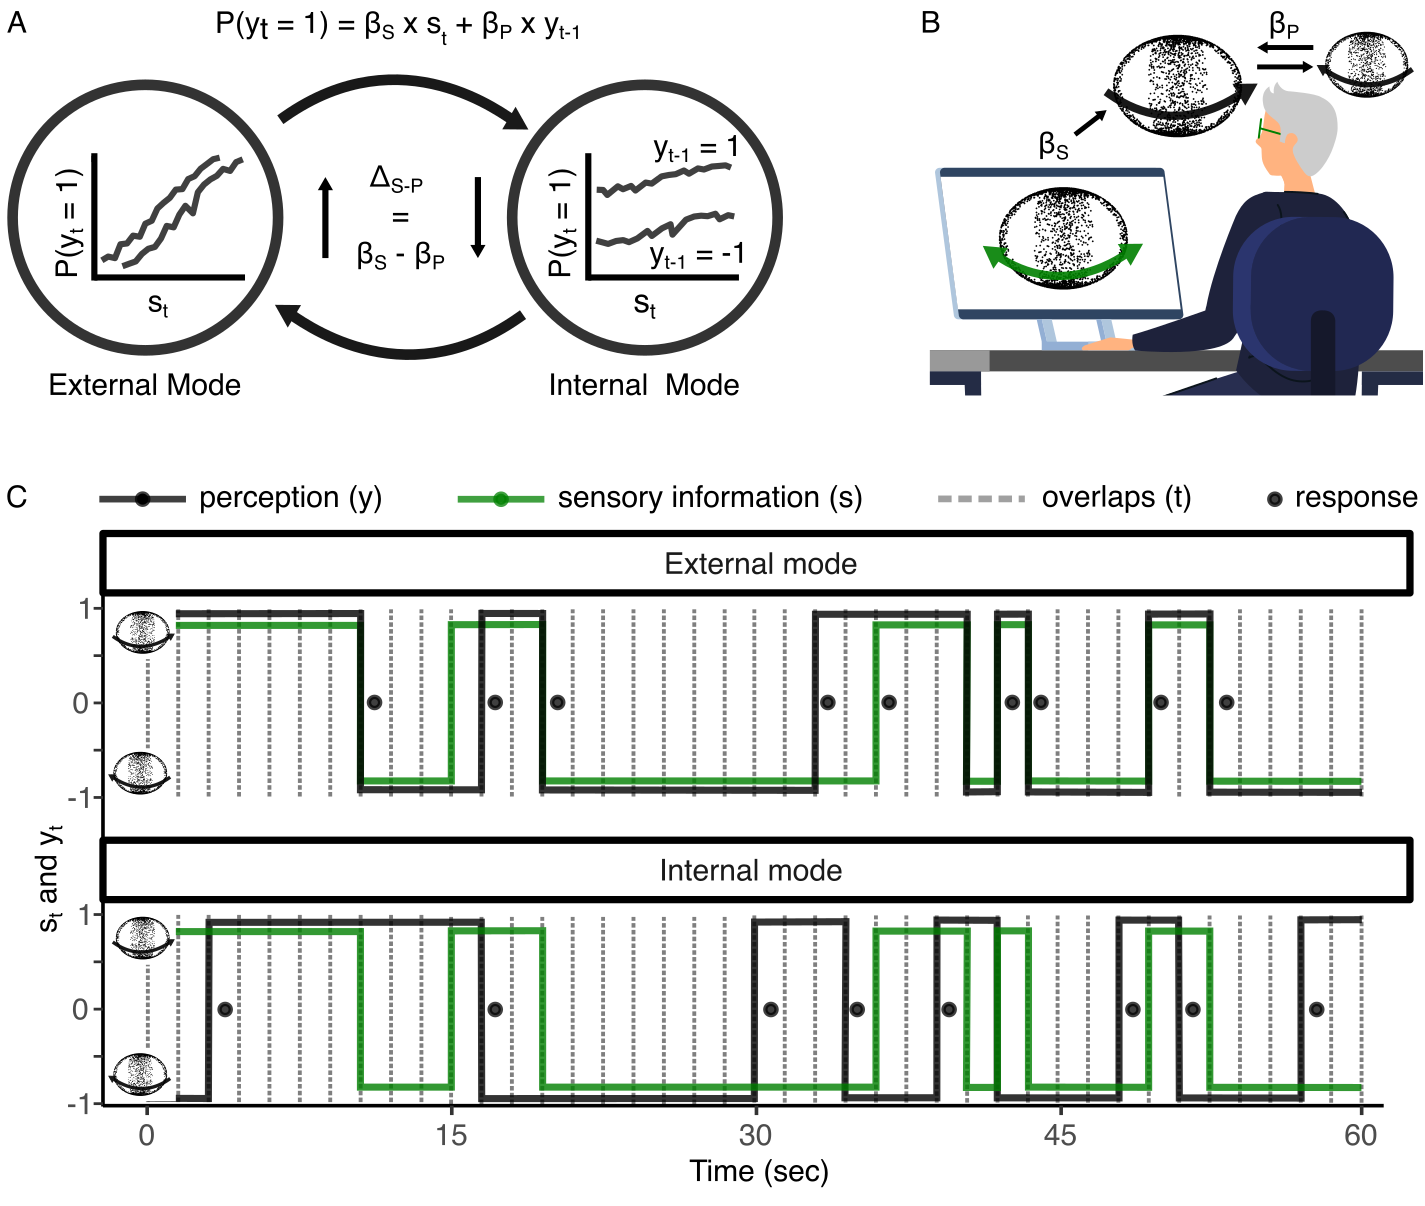
\includegraphics{./modes_ketamine_scz_files/figure-latex/Figure_1.png}

\begin{itemize}
\item
  \textbf{Figure 1.}
\item
  \textbf{A.} \textbf{Perception integrates ambiguous sensory signals
  \(s_t\) with internal predictions that reflect prior knowledge about
  the world. One source of prior knowledge is the temporal
  autocorrelation of natural environments, where the recent past often
  predicts the near future. The integration of external inputs and
  internal predictions depends on the weights assigned to incoming
  sensory data (\(\beta_S \times s_t\)) and to internal prediction
  derived from previous experiences (\(\beta_P \times y_{t-1}\), dotted
  versus solid lines, simulated data), respectively. \(\beta_S\)
  determines the slope, and \(\beta_P\) the shift of the psychometric
  function that links \(s_t\) and \(y_t\). Importantly, the balance
  \(\Delta_{S-P} = \beta_S - \beta_P\) is known to alternate between two
  opposing modes: During the external mode (left), perception is largely
  determined by \(\beta_S \times s_t\), which is reflected by a steep
  slope and a small shift of the psychometric curve. Conversely, during
  the internal mode (right), perception is shaped by
  \(\beta_P \times y_{t-1}\), resulting in a shallow slope and a large
  shift of the psychometric curve.}
\item
  \textbf{B.} \textbf{We conducted a double-blind placebo-controlled
  experiments in 28 healthy human participants, who received a
  continuous infusion with either the NMDAR antagonist S-ketamine or
  saline. During the infusion, the participants viewed SFM stimuli at
  varying levels of signal-to-ambiguity (SAR). The stimuli were
  compatible with two mutually exclusive subjective experiences (left
  vs.~rightward rotation of the front surface, green arrows). Fully
  ambiguous stimuli (SAR = 0) induce the phenomenon of bistable
  perception, where participants perceive spontaneous changes between
  the two possible interpretations of the stimulus (black arrows) at a
  rate that is governed by \(\beta_P\), the degree to which perception
  is shaped by internal predictions derived from previous experiences.
  For partially ambiguous stimuli (SAR \textgreater{} 0), perception
  reflects the weighted integration of internal predictions with
  external sensory data, which is governed by the balance
  \(\Delta_{S-P} = \beta_S - \beta_P\).}
\item
  \textbf{C.} \textbf{Changes in the perceived direction of rotation of
  the SFM stimulus occur at brief depth-symmetric configurations of the
  stimulus (grey dotted lines; Supplemental Video S1). We transformed
  the behavioral responses into a sequence of states \(t\) (80 1.5 sec
  intervals per block), each associated with a combination of the
  SAR-weighted input \(s_t\) (green line) and the perceived direction of
  rotation \(y_t\) (black line). Participants reported whenever they
  experienced a change in conscious experience (black dots). The
  response times \(r_t\) was defined as the lag between the response and
  the last preceding overlap. We used HMM-GLMs to quantify the weights
  \(\beta_S\), \(\beta_P\) and \(\beta_B\), which reflect how the
  reported percepts \(y_t\) were determined by the external inputs
  \(\beta_S \times s_t\), the internal predictions
  \(\beta_P \times y_{t-1}\), and the constant bias
  \(\beta_B \times 1\), separately for the external mode (upper panel,
  60 sec of example data) and the internal mode (lower panel, 60 sec of
  example data with identical \(s(t)\) for visualization). In the
  external mode, perception follows the external stimulus closely (high
  \(\Delta_{S-P} = \beta_S - \beta_P\)). In the internal mode,
  perception is shaped more strongly by internal predictions derived
  from previous experiences (low \(\Delta_{S-P} = \beta_S - \beta_P\)).}
\end{itemize}

\subsubsection{Comment 2}\label{comment-2-3}

\textbf{Analyses of individual differences: The authors note that their
``experiments maximized intra-subject power and were not designed to
detect inter-individual differences.'' However in their previous work
using the same dataset (Weilnhammer et al., 2020) they did explore
interindividual differences and found a significant positive
relationship between hallucination severity and an analogous model
parameter. Regardless of whether a similar finding holds true with their
new modeling approach, it is important to show the results of a similar
analysis to contextualize their findings.}

Thanks a lot for pointing this out. In Weilnhammer et al.~2020, we found
that psychosis proneness correlated with the gain of sensory processing.
The gain variable reflected how much the accuracy of perception
increases as a function of signal-to-ambiguity ratio. We agree that it
is an interesting question for future research whether the balance
between modes is, like gain, correlated to psychosis-proneness. However,
in this analysis, we did not find such a correlation. We feel that the
sample size is too small to make a strong statement based on the absence
of a significant correlation. The respective plots are shown in
Supplemental Figure S7.

\begin{itemize}
\tightlist
\item
  \textbf{D.} Neither PDI, CAPS, nor 5-ASC scores were predictive of the
  probability of external mode (shown separately for S-ketamine in red
  and placebo in blue).
\end{itemize}

\subsubsection{Comment 3}\label{comment-3-3}

\textbf{Choice history effects: As evidence that changes in responding
represent differences in perception rather differences in choice
persistence, the authors rely on: (i) prior literature which they note
shows evidence of choice history effects and argue that choice
persistence is unlikely in their paradigm because it does not require
choices at every stimulus overlap, only following changes of mind. It is
not clear to me that the brain mechanisms underlying choice persistence
would simply be disengaged by the requirement to only report changes of
mind. (ii) Perform an analysis showing that the current perceptual
experience is better explained by previous `perceptual experience' than
by previous stimulus. This is interesting but does not rule out the
contribution of previous choice because choice and percept are
intertwined. (iii) perform an analysis of confidence showing that
confidence reports are predicted by posterior certainty. Unfortunately,
this is also what I would expect to be predicted by a simpler model of
choice persistence. Again, the reason is that posterior certainty
depends on the prior i.e., previous posterior. Because the model does
not have an explicit choice-history term, any effect of choice
persistence would necessarily be absorbed into the previous posterior,
masquerading as a perceptual phenomenon. (iv) Demonstrate that
metacognitive performance (quantified as the correlation between
confidence and perceptual accuracy) is worse in the internal mode. This
result can also be alternatively attributed to choice persistence since
the latter decouples behavioral choices from external input.}

\textbf{Thus, while I appreciate the new analyses based on confidence,
the interpretation of these results solely as a perceptual phenomenon
seems largely due to the formulation of the GLM. To conclusively
decouple choice persistence and perception, the authors might want to
fit a GLM that incorporates the previous confidence report (proxy for
subjective belief) in addition to the previous perceptual choice and
stimulus. Ideally, the weighting on the previous choice would not be
different across the two modes. Alternatively, the claims equating
ketamine-induced alterations in mode dynamics to perceptual abnormality
should be toned done further throughout the paper, allowing for the
possibility of addressing the confound of choice persistence in future
work.}

We thank the reviewer for this clarification. We would like to emphasize
that unlike paradigms in which participants perform perceptual choices
at each trial, participants in our experiments did not make choices at
every stimulus overlap, but only at a fraction of overlaps, whenever
they experienced changes in perception (see Figure 1C). Our results
therefore cannot be explained by actual choice persistence from trial to
trial (or, in our case, overlap to overlap). Still, we agree that it is
challenging to distinguish with certainty genuine perceptual changes
from potential fluctuations in response behavior, because perception and
report are naturally intertwined in our paradigm. It is important for
future work to disentangle perception and response behavior with respect
to modes. We feel this is a broader, open question in research on
bistable perception, the neural correlates of conscious experience, and
in our present analysis of mode dynamics, as all these areas equate
responses with the content of perception.

Following the reviewer's suggestion, we have revised the manuscript to
highlight the importance of future research in disentangling response
behavior from perceptual phenomena. Additionally, we have clarified
throughout the paper that while our findings on mode dynamics suggest a
relationship with perception, they do not rule out potential
contributions of report-related effects. The following changes have been
made to the manuscript:

\begin{itemize}
\item
  Methods section: lease note that we assessed participants' perception
  of the stimulus based on a fixed response mapping. In our paradigm,
  perception and reports are therefore inherently intertwined, with the
  participants' reports serving as the sole indicators of their
  perceptual states.
\item
  Methods: Please note that the interpretation of our results is
  inherently limited to the hypotheses incorporated in the above GLMs.
  In our paradigm, behavioral reports at the time of changes in
  experience served as the only indicators of the perceptual and
  metacognitive states of the participants. These behavioral reports
  were collected with a fixed stimulus-response mapping, such that the
  GLM-based analyses cannot fully separate perception and response
  behavior.
\item
  Results: Our results suggest that healthy participants under
  S-ketamine and Scz patients spend more time in the external mode. As a
  dynamic mechanism for psychotic experiences, alternations between
  external and internal mode should have an effect at the level of
  perception. This means that between-mode alternations should modulate
  a perceptual decision variable that determines not only what is
  consciously experienced, but also how the contents of perception are
  evaluated by downstream cognition. The hypothesis that external and
  internal modes are perceptual phenomena needs to be contrasted against
  alternative scenarios in which external and internal modes are driven
  primarily by fluctuations in arousal, high-level cognition, or
  executive function. This is particularly important, as behavioral
  reports served as the sole indicators of perceptual states in our
  paradigm.
\end{itemize}

Furthermore, we acknowledge the potential utility of fitting a more
comprehensive GLM model that incorporates previous confidence reports,
previous perceptual choices, and stimulus history, as suggested by the
reviewer. In the present data, however, we collected reports of
perceptual content and confidence only at the time of changes in
perception. To conclusively answer the reviewer's point, future
experiment need gather perceptual reports and confidence at every
overlap / trial. We followed the reviewer's suggestion and stress the
importance of addressing the choice persistence confound in future work
in the discussion:

\begin{itemize}
\tightlist
\item
  Discussion (\ldots) These observations do not, however, rule out the
  possibility that external and internal modes have multiple and
  potentially independent effects on the brain, including influences on
  high-level cognition and response behavior, or that they are, to some
  degree, dependent on global brain states. Since our analyses rely on
  behavioral reports about changes in the content of perception, dynamic
  changes in response behavior represent an additional potential
  confound in the identification of external and internal modes. Future
  work should use trial-wise reports of perception and confidence with
  randomized response mappings to enable GLMs that can disentangle
  perception and response behavior. No-report functional imaging
  experiments, where the content of experiences is decoded without overt
  behavioral signals\textsuperscript{70}, alongside pupillometry,
  manipulations of neuromodulators that regulate global brain states, or
  non-invasive brain stimulation, could help illuminate the causes and
  consequences of these modes across the cortical hierarchy. Mapping the
  neurocomputational dynamics of mode alternations will be crucial to
  testing whether adjusting the balance between modes can mitigate
  psychotic experiences and ultimately improve the lives of people
  living with Scz.
\end{itemize}

\newpage

\section*{References}\label{references}
\addcontentsline{toc}{section}{References}

\phantomsection\label{refs}
\begin{CSLReferences}{0}{0}
\bibitem[\citeproctext]{ref-Sterzer2018}
\CSLLeftMargin{1. }%
\CSLRightInline{Sterzer, P. \emph{et al.}
\href{https://doi.org/10.1016/j.biopsych.2018.05.015}{The {Predictive}
{Coding} {Account} of {Psychosis}}. \emph{Biological Psychiatry}
\textbf{84}, 634--643 (2018).}

\bibitem[\citeproctext]{ref-fletcher_perceiving_2009}
\CSLLeftMargin{2. }%
\CSLRightInline{Fletcher, P. C. \emph{et al.}
\href{https://doi.org/10.1038/nrn2536}{Perceiving is believing: A
{Bayesian} approach to explaining the positive symptoms of
schizophrenia}. \emph{Nature Reviews Neuroscience} \textbf{10}, 48--58
(2009).}

\bibitem[\citeproctext]{ref-Adams2013}
\CSLLeftMargin{3. }%
\CSLRightInline{Adams, R. A. \emph{et al.}
\href{https://doi.org/10.3389/fpsyt.2013.00047}{The computational
anatomy of psychosis.} \emph{Frontiers in psychiatry} \textbf{4}, 47
(2013).}

\bibitem[\citeproctext]{ref-Friston2005}
\CSLLeftMargin{4. }%
\CSLRightInline{Friston, K.
\href{https://doi.org/10.1098/rstb.2005.1622}{A theory of cortical
responses.} \emph{Philosophical transactions of the Royal Society of
London. Series B, Biological sciences} \textbf{360}, 815--836 (2005).}

\bibitem[\citeproctext]{ref-Rao1999}
\CSLLeftMargin{5. }%
\CSLRightInline{Rao, R. P. \emph{et al.}
\href{https://doi.org/10.1038/4580}{Predictive coding in the visual
cortex: A functional interpretation of some extra-classical
receptive-field effects.} \emph{Nature neuroscience} \textbf{2}, 79--87
(1999).}

\bibitem[\citeproctext]{ref-Friston2009a}
\CSLLeftMargin{6. }%
\CSLRightInline{Friston, K. \emph{et al.}
\href{https://doi.org/10.1098/rstb.2008.0300}{Predictive coding under
the free-energy principle}. \emph{Philosophical Transactions of the
Royal Society B: Biological Sciences} \textbf{364}, 1211--1221 (2009).}

\bibitem[\citeproctext]{ref-feldman_attention_2010}
\CSLLeftMargin{7. }%
\CSLRightInline{Feldman, H. \emph{et al.}
\href{https://doi.org/10.3389/FNHUM.2010.00215/BIBTEX}{Attention,
uncertainty, and free-energy}. \emph{Frontiers in Human Neuroscience}
\textbf{4}, 7028 (2010).}

\bibitem[\citeproctext]{ref-moran_losing_2015}
\CSLLeftMargin{8. }%
\CSLRightInline{Moran, R. J. \emph{et al.}
\href{https://doi.org/10.1038/npp.2014.184}{Losing {Control} {Under}
{Ketamine}: {Suppressed} {Cortico}-{Hippocampal} {Drive} {Following}
{Acute} {Ketamine} in {Rats}}. \emph{Neuropsychopharmacology}
\textbf{40}, 268--277 (2015).}

\bibitem[\citeproctext]{ref-muthukumaraswamy_evidence_2015}
\CSLLeftMargin{9. }%
\CSLRightInline{Muthukumaraswamy, S. D. \emph{et al.}
\href{https://doi.org/10.1523/JNEUROSCI.0903-15.2015}{Evidence that
{Subanesthetic} {Doses} of {Ketamine} {Cause} {Sustained} {Disruptions}
of {NMDA} and {AMPA}-{Mediated} {Frontoparietal} {Connectivity} in
{Humans}}. \emph{Journal of Neuroscience} \textbf{35}, 11694--11706
(2015).}

\bibitem[\citeproctext]{ref-powers_iii_ketamine-induced_2015}
\CSLLeftMargin{10. }%
\CSLRightInline{Powers III, A. R. \emph{et al.}
\href{https://doi.org/10.1159/000438675}{Ketamine-{Induced}
{Hallucinations}}. \emph{Psychopathology} \textbf{48}, 376--385 (2015).}

\bibitem[\citeproctext]{ref-ranlund_impaired_2016}
\CSLLeftMargin{11. }%
\CSLRightInline{Ranlund, S. \emph{et al.}
\href{https://doi.org/10.1002/hbm.23035}{Impaired prefrontal synaptic
gain in people with psychosis and their relatives during the mismatch
negativity}. \emph{Human Brain Mapping} \textbf{37}, 351--365 (2016).}

\bibitem[\citeproctext]{ref-corlett_glutamatergic_2011}
\CSLLeftMargin{12. }%
\CSLRightInline{Corlett, P. R. \emph{et al.}
\href{https://doi.org/10.1038/npp.2010.163}{Glutamatergic {Model}
{Psychoses}: {Prediction} {Error}, {Learning}, and {Inference}}.
\emph{Neuropsychopharmacology} \textbf{36}, 294--315 (2011).}

\bibitem[\citeproctext]{ref-Stein2020}
\CSLLeftMargin{13. }%
\CSLRightInline{Stein, H. \emph{et al.}
\href{https://doi.org/10.1038/s41467-020-18033-3}{Reduced serial
dependence suggests deficits in synaptic potentiation in anti-{NMDAR}
encephalitis and schizophrenia}. \emph{Nature Communications}
\textbf{11}, 1--11 (2020).}

\bibitem[\citeproctext]{ref-murray_linking_2014}
\CSLLeftMargin{14. }%
\CSLRightInline{Murray, J. D. \emph{et al.}
\href{https://doi.org/10.1093/cercor/bhs370}{Linking {Microcircuit}
{Dysfunction} to {Cognitive} {Impairment}: {Effects} of {Disinhibition}
{Associated} with {Schizophrenia} in a {Cortical} {Working} {Memory}
{Model}}. \emph{Cerebral Cortex} \textbf{24}, 859--872 (2014).}

\bibitem[\citeproctext]{ref-catts_quantitative_2016}
\CSLLeftMargin{15. }%
\CSLRightInline{Catts, V. S. \emph{et al.}
\href{https://doi.org/10.1016/j.biopsycho.2015.10.013}{A quantitative
review of the postmortem evidence for decreased cortical
{N}-methyl-{D}-aspartate receptor expression levels in schizophrenia:
{How} can we link molecular abnormalities to mismatch negativity
deficits?} \emph{Biological Psychology} \textbf{116}, 57--67 (2016).}

\bibitem[\citeproctext]{ref-wang_nmda_2013}
\CSLLeftMargin{16. }%
\CSLRightInline{Wang, M. \emph{et al.}
\href{https://doi.org/10.1016/j.neuron.2012.12.032}{{NMDA} {Receptors}
{Subserve} {Persistent} {Neuronal} {Firing} during {Working} {Memory} in
{Dorsolateral} {Prefrontal} {Cortex}}. \emph{Neuron} \textbf{77},
736--749 (2013).}

\bibitem[\citeproctext]{ref-self_different_2012}
\CSLLeftMargin{17. }%
\CSLRightInline{Self, M. W. \emph{et al.}
\href{https://doi.org/10.1073/pnas.1119527109}{Different glutamate
receptors convey feedforward and recurrent processing in macaque {V1}}.
\emph{Proceedings of the National Academy of Sciences} \textbf{109},
11031--11036 (2012).}

\bibitem[\citeproctext]{ref-castro-alamancos_short-term_1996}
\CSLLeftMargin{18. }%
\CSLRightInline{Castro-Alamancos, M. A. \emph{et al.}
\href{https://doi.org/10.1073/pnas.93.3.1335}{Short-term synaptic
enhancement and long-term potentiation in neocortex.} \emph{Proceedings
of the National Academy of Sciences} \textbf{93}, 1335--1339 (1996).}

\bibitem[\citeproctext]{ref-nakazawa_spatial_2017}
\CSLLeftMargin{19. }%
\CSLRightInline{Nakazawa, K. \emph{et al.}
\href{https://doi.org/10.1038/s41537-016-0003-3}{Spatial and temporal
boundaries of {NMDA} receptor hypofunction leading to schizophrenia}.
\emph{npj Schizophrenia} \textbf{3}, 1--11 (2017).}

\bibitem[\citeproctext]{ref-jardri_cortical_2011}
\CSLLeftMargin{20. }%
\CSLRightInline{Jardri, R. \emph{et al.}
\href{https://doi.org/10.1176/appi.ajp.2010.09101522}{Cortical
activations during auditory verbal hallucinations in schizophrenia: A
coordinate-based meta-analysis}. \emph{The American Journal of
Psychiatry} \textbf{168}, 73--81 (2011).}

\bibitem[\citeproctext]{ref-zmigrod_neural_2016}
\CSLLeftMargin{21. }%
\CSLRightInline{Zmigrod, L. \emph{et al.}
\href{https://doi.org/10.1016/j.neubiorev.2016.05.037}{The neural
mechanisms of hallucinations: {A} quantitative meta-analysis of
neuroimaging studies}. \emph{Neuroscience and Biobehavioral Reviews}
\textbf{69}, 113--123 (2016).}

\bibitem[\citeproctext]{ref-gill_real-time_2022}
\CSLLeftMargin{22. }%
\CSLRightInline{Gill, K. \emph{et al.}
\href{https://doi.org/10.1093/schizbullopen/sgac050}{Real-{Time}
{Symptom} {Capture} of {Hallucinations} in {Schizophrenia} with {fMRI}:
{Absence} of {Duration}-{Dependent} {Activity}}. \emph{Schizophrenia
Bulletin Open} \textbf{3}, sgac050 (2022).}

\bibitem[\citeproctext]{ref-laquitaine_switching_2018}
\CSLLeftMargin{23. }%
\CSLRightInline{Laquitaine, S. \emph{et al.}
\href{https://doi.org/10.1016/j.neuron.2017.12.011}{A {Switching}
{Observer} for {Human} {Perceptual} {Estimation}}. \emph{Neuron}
\textbf{97}, 462--474.e6 (2018).}

\bibitem[\citeproctext]{ref-roy_extracting_2021}
\CSLLeftMargin{24. }%
\CSLRightInline{Roy, N. A. \emph{et al.}
\href{https://doi.org/10.1016/J.NEURON.2020.12.004}{Extracting the
dynamics of behavior in sensory decision-making experiments}.
\emph{Neuron} \textbf{109}, 597--610.e6 (2021).}

\bibitem[\citeproctext]{ref-ashwood_mice_2022}
\CSLLeftMargin{25. }%
\CSLRightInline{Ashwood, Z. C. \emph{et al.}
\href{https://doi.org/10.1038/s41593-021-01007-z}{Mice alternate between
discrete strategies during perceptual decision-making}. \emph{Nature
Neuroscience} \textbf{25}, 201--212 (2022).}

\bibitem[\citeproctext]{ref-weilnhammer_sensory_2023}
\CSLLeftMargin{26. }%
\CSLRightInline{Weilnhammer, V. \emph{et al.}
\href{https://doi.org/10.1371/journal.pbio.3002410}{Sensory processing
in humans and mice fluctuates between external and internal modes}.
\emph{PLOS Biology} \textbf{21}, e3002410 (2023).}

\bibitem[\citeproctext]{ref-albert_hierarchical_2017}
\CSLLeftMargin{27. }%
\CSLRightInline{Albert, S. \emph{et al.}
\href{https://doi.org/10.1371/journal.pcbi.1005856}{A hierarchical
stochastic model for bistable perception}. \emph{PLOS Computational
Biology} \textbf{13}, e1005856 (2017).}

\bibitem[\citeproctext]{ref-weilnhammer_psychotic_2020}
\CSLLeftMargin{28. }%
\CSLRightInline{Weilnhammer, V. \emph{et al.}
\href{http://www.ncbi.nlm.nih.gov/pubmed/32090246}{Psychotic
{Experiences} in {Schizophrenia} and {Sensitivity} to {Sensory}
{Evidence}.} \emph{Schizophrenia bulletin} \textbf{46}, 927--936
(2020).}

\bibitem[\citeproctext]{ref-Peters1999}
\CSLLeftMargin{29. }%
\CSLRightInline{Peters, E. R. \emph{et al.}
\href{https://www.ncbi.nlm.nih.gov/pubmed/10478789}{Measurement of
delusional ideation in the normal population: Introducing the {PDI}
({Peters} et al. {Delusions} {Inventory}).} \emph{Schizophrenia
bulletin} \textbf{25}, 553--76 (1999).}

\bibitem[\citeproctext]{ref-Bell2006}
\CSLLeftMargin{30. }%
\CSLRightInline{Bell, V. \emph{et al.}
\href{https://doi.org/10.1093/schbul/sbj014}{The {Cardiff} {Anomalous}
{Perceptions} {Scale} ({CAPS}): {A} {New} {Validated} {Measure} of
{Anomalous} {Perceptual} {Experience}}. \emph{Schizophrenia Bulletin}
\textbf{32}, 366--377 (2006).}

\bibitem[\citeproctext]{ref-overall_brief_1962}
\CSLLeftMargin{31. }%
\CSLRightInline{Overall, J. E. \emph{et al.}
\href{https://doi.org/10.2466/pr0.1962.10.3.799}{The {Brief}
{Psychiatric} {Rating} {Scale}}. \emph{Psychological Reports}
\textbf{10}, 799--812 (1962).}

\bibitem[\citeproctext]{ref-Brainard1997}
\CSLLeftMargin{32. }%
\CSLRightInline{Brainard, D. H.
\href{https://www.ncbi.nlm.nih.gov/pubmed/9176952}{The {Psychophysics}
{Toolbox}.} \emph{Spatial vision} \textbf{10}, 433--6 (1997).}

\bibitem[\citeproctext]{ref-weilnhammer_active_2021}
\CSLLeftMargin{33. }%
\CSLRightInline{Weilnhammer, V. \emph{et al.}
\href{https://doi.org/10.1016/j.cub.2021.04.043}{An active role of
inferior frontal cortex in conscious experience}. \emph{Current Biology}
\textbf{31}, 2868--2880.e8 (2021).}

\bibitem[\citeproctext]{ref-mertens_clinician-administered_2022}
\CSLLeftMargin{34. }%
\CSLRightInline{Mertens, Y. L. \emph{et al.}
\href{https://doi.org/10.1080/15299732.2021.1989111}{The
{Clinician}-{Administered} {Dissociative} {States} {Scale} ({CADSS}):
{Validation} of the {German} {Version}}. \emph{Journal of Trauma \&
Dissociation} \textbf{23}, 366--384 (2022).}

\bibitem[\citeproctext]{ref-dittrich_5d-abz_1999}
\CSLLeftMargin{35. }%
\CSLRightInline{Dittrich, A. \emph{et al.} {5D}-{ABZ}: {Fragebogen} zur
{Erfassung} {Aussergewöhnlicher} {Bewusstseinszustände}. \emph{Eine
kurze Einführung. PSIN Plus, Zürich} (1999).}

\bibitem[\citeproctext]{ref-Kay1987}
\CSLLeftMargin{36. }%
\CSLRightInline{Kay, S. R. \emph{et al.}
\href{https://www.ncbi.nlm.nih.gov/pubmed/3616518}{The positive and
negative syndrome scale ({PANSS}) for schizophrenia.}
\emph{Schizophrenia bulletin} \textbf{13}, 261--76 (1987).}

\bibitem[\citeproctext]{ref-manassi_continuity_2024}
\CSLLeftMargin{37. }%
\CSLRightInline{Manassi, M. \emph{et al.}
\href{https://doi.org/10.1038/s44159-024-00297-x}{Continuity fields
enhance visual perception through positive serial dependence}.
\emph{Nature Reviews Psychology} \textbf{3}, 352--366 (2024).}

\bibitem[\citeproctext]{ref-shergill_evidence_2005}
\CSLLeftMargin{38. }%
\CSLRightInline{Shergill, S. S. \emph{et al.}
\href{https://doi.org/10.1176/appi.ajp.162.12.2384}{Evidence for sensory
prediction deficits in schizophrenia}. \emph{The American Journal of
Psychiatry} \textbf{162}, 2384--2386 (2005).}

\bibitem[\citeproctext]{ref-keane_reduced_2013}
\CSLLeftMargin{39. }%
\CSLRightInline{Keane, B. P. \emph{et al.}
\href{https://doi.org/10.1037/a0032110}{Reduced depth inversion
illusions in schizophrenia are state-specific and occur for multiple
object types and viewing conditions}. \emph{Journal of abnormal
psychology} \textbf{122}, 506--512 (2013).}

\bibitem[\citeproctext]{ref-Silverstein2013}
\CSLLeftMargin{40. }%
\CSLRightInline{Silverstein, S. \emph{et al.}
\href{https://doi.org/10.1167/13.9.1261}{Reduced {Sensitivity} to the
{Ebbinghaus} {Illusion} is {State} {Related} in {Schizophrenia}}.
\emph{Journal of Vision} \textbf{13}, 1261--1261 (2013).}

\bibitem[\citeproctext]{ref-Pastukhov2012}
\CSLLeftMargin{41. }%
\CSLRightInline{Pastukhov, A. \emph{et al.}
\href{https://doi.org/10.1167/12.1.17}{Believable change: Bistable
reversals are governed by physical plausibility.} \emph{Journal of
vision} \textbf{12}, 17 (2012).}

\bibitem[\citeproctext]{ref-weilnhammer_predictive_2017}
\CSLLeftMargin{42. }%
\CSLRightInline{Weilnhammer, V. \emph{et al.}
\href{https://doi.org/10.1371/journal.pcbi.1005536}{A predictive coding
account of bistable perception - a model-based {fMRI} study}. \emph{PLOS
Computational Biology} \textbf{13}, e1005536 (2017).}

\bibitem[\citeproctext]{ref-Fleming2014}
\CSLLeftMargin{43. }%
\CSLRightInline{Fleming, S. M. \emph{et al.}
\href{https://doi.org/10.3389/fnhum.2014.00443}{How to measure
metacognition}. \emph{Frontiers in Human Neuroscience} \textbf{8}, 443
(2014).}

\bibitem[\citeproctext]{ref-linderman_ssm_2020}
\CSLLeftMargin{44. }%
\CSLRightInline{Linderman, S. \emph{et al.}
\href{https://github.com/lindermanlab/ssm}{{SSM}: {Bayesian} {Learning}
and {Inference} for {State} {Space} {Models}}. (2020).}

\bibitem[\citeproctext]{ref-Hohwy2008}
\CSLLeftMargin{45. }%
\CSLRightInline{Hohwy, J. \emph{et al.}
\href{https://doi.org/10.1016/j.cognition.2008.05.010}{Predictive coding
explains binocular rivalry: An epistemological review.} \emph{Cognition}
\textbf{108}, 687--701 (2008).}

\bibitem[\citeproctext]{ref-Hohwy2012}
\CSLLeftMargin{46. }%
\CSLRightInline{Hohwy, J.
\href{https://doi.org/10.3389/fpsyg.2012.00096}{Attention and conscious
perception in the hypothesis testing brain.} \emph{Frontiers in
psychology} \textbf{3}, 96 (2012).}

\bibitem[\citeproctext]{ref-adams_computational_2022}
\CSLLeftMargin{47. }%
\CSLRightInline{Adams, R. A. \emph{et al.}
\href{https://doi.org/10.1016/j.biopsych.2021.07.024}{Computational
{Modeling} of {Electroencephalography} and {Functional} {Magnetic}
{Resonance} {Imaging} {Paradigms} {Indicates} a {Consistent} {Loss} of
{Pyramidal} {Cell} {Synaptic} {Gain} in {Schizophrenia}}.
\emph{Biological Psychiatry} \textbf{91}, 202--215 (2022).}

\bibitem[\citeproctext]{ref-blakemore_spatio-temporal_1999}
\CSLLeftMargin{48. }%
\CSLRightInline{Blakemore, S. J. \emph{et al.}
\href{https://doi.org/10.1162/089892999563607}{Spatio-temporal
prediction modulates the perception of self-produced stimuli}.
\emph{Journal of Cognitive Neuroscience} \textbf{11}, 551--559 (1999).}

\bibitem[\citeproctext]{ref-limanowski_dis-_2017}
\CSLLeftMargin{49. }%
\CSLRightInline{Limanowski, J.
\emph{\href{https://openscience.ub.uni-mainz.de/handle/20.500.12030/643}{({Dis}-)
attending to the {Body}: {Action} and {Self}-experience in the {Active}
{Inference} {Framework}}}. (Johannes Gutenberg-Universität Mainz
Frankfurt am Main, 2017).}

\bibitem[\citeproctext]{ref-oestreich_subnormal_2015}
\CSLLeftMargin{50. }%
\CSLRightInline{Oestreich, L. K. L. \emph{et al.}
\href{https://doi.org/10.1016/j.ijpsycho.2015.05.014}{Subnormal sensory
attenuation to self-generated speech in schizotypy:
{Electrophysiological} evidence for a 'continuum of psychosis'}.
\emph{International Journal of Psychophysiology: Official Journal of the
International Organization of Psychophysiology} \textbf{97}, 131--138
(2015).}

\bibitem[\citeproctext]{ref-mathys_bayesian_2011}
\CSLLeftMargin{51. }%
\CSLRightInline{Mathys, C. \emph{et al.}
\href{https://doi.org/10.3389/fnhum.2011.00039}{A {Bayesian}
{Foundation} for {Individual} {Learning} {Under} {Uncertainty}}.
\emph{Frontiers in Human Neuroscience} \textbf{5}, (2011).}

\bibitem[\citeproctext]{ref-Iglesias2013}
\CSLLeftMargin{52. }%
\CSLRightInline{Iglesias, S. \emph{et al.}
\href{https://doi.org/10.1016/j.neuron.2013.09.009}{Hierarchical
{Prediction} {Errors} in {Midbrain} and {Basal} {Forebrain} during
{Sensory} {Learning}}. \emph{Neuron} \textbf{80}, 519--530 (2013).}

\bibitem[\citeproctext]{ref-kucyi_spontaneous_2016}
\CSLLeftMargin{53. }%
\CSLRightInline{Kucyi, A. \emph{et al.}
\href{https://doi.org/10.1073/pnas.1611743113}{Spontaneous default
network activity reflects behavioral variability independent of
mind-wandering}. \emph{Proceedings of the National Academy of Sciences}
\textbf{113}, 13899--13904 (2016).}

\bibitem[\citeproctext]{ref-yamashita_variable_2021}
\CSLLeftMargin{54. }%
\CSLRightInline{Yamashita, A. \emph{et al.}
\href{https://doi.org/10.1038/s41598-021-94161-0}{Variable rather than
extreme slow reaction times distinguish brain states during sustained
attention}. \emph{Scientific Reports} \textbf{11}, 14883 (2021).}

\bibitem[\citeproctext]{ref-weilnhammer_bistable_2021}
\CSLLeftMargin{55. }%
\CSLRightInline{Weilnhammer, V. \emph{et al.}
\href{https://doi.org/10.1016/j.isci.2021.102234}{Bistable perception
alternates between internal and external modes of sensory processing}.
\emph{iScience} \textbf{24}, 102234 (2021).}

\bibitem[\citeproctext]{ref-weilnhammer_dynamic_2024}
\CSLLeftMargin{56. }%
\CSLRightInline{Weilnhammer, V. \emph{et al.}
\href{https://doi.org/10.1016/j.cub.2024.07.087}{Dynamic predictive
templates in perception}. \emph{Current Biology} \textbf{0}, (2024).}

\bibitem[\citeproctext]{ref-muckli_contextual_2015}
\CSLLeftMargin{57. }%
\CSLRightInline{Muckli, L. \emph{et al.}
\href{https://doi.org/10.1016/j.cub.2015.08.057}{Contextual {Feedback}
to {Superficial} {Layers} of {V1}}. \emph{Current Biology} \textbf{25},
2690--2695 (2015).}

\bibitem[\citeproctext]{ref-weilnhammer_neural_2018}
\CSLLeftMargin{58. }%
\CSLRightInline{Weilnhammer, V. \emph{et al.}
\href{https://doi.org/10.1523/JNEUROSCI.2901-17.2018}{The {Neural}
{Correlates} of {Hierarchical} {Predictions} for {Perceptual}
{Decisions}}. \emph{The Journal of Neuroscience} \textbf{38}, 5008--5021
(2018).}

\bibitem[\citeproctext]{ref-Notredame2014}
\CSLLeftMargin{59. }%
\CSLRightInline{Notredame, C.-E. \emph{et al.}
\href{https://doi.org/10.3389/fnint.2014.00063}{What visual illusions
teach us about schizophrenia.} \emph{Frontiers in integrative
neuroscience} \textbf{8}, 63 (2014).}

\bibitem[\citeproctext]{ref-costa_systematic_2023}
\CSLLeftMargin{60. }%
\CSLRightInline{Costa, A. L. L. \emph{et al.}
\href{https://doi.org/10.1016/j.schres.2022.12.030}{Systematic review of
visual illusions in schizophrenia}. \emph{Schizophrenia Research}
\textbf{252}, 13--22 (2023).}

\bibitem[\citeproctext]{ref-cassidy_perceptual_2018}
\CSLLeftMargin{61. }%
\CSLRightInline{Cassidy, C. M. \emph{et al.}
\href{https://doi.org/10.1016/j.cub.2017.12.059}{A {Perceptual}
{Inference} {Mechanism} for {Hallucinations} {Linked} to {Striatal}
{Dopamine}}. \emph{Current Biology} \textbf{28}, 503--514.e4 (2018).}

\bibitem[\citeproctext]{ref-schmack_striatal_2021}
\CSLLeftMargin{62. }%
\CSLRightInline{Schmack, K. \emph{et al.}
\href{https://doi.org/10.1126/science.abf4740}{Striatal dopamine
mediates hallucination-like perception in mice}. \emph{Science (New
York, N.Y.)} \textbf{372}, eabf4740 (2021).}

\bibitem[\citeproctext]{ref-bansal_association_2022}
\CSLLeftMargin{63. }%
\CSLRightInline{Bansal, S. \emph{et al.}
\href{https://doi.org/10.1001/jamapsychiatry.2021.3482}{Association
{Between} {Failures} in {Perceptual} {Updating} and the {Severity} of
{Psychosis} in {Schizophrenia}}. \emph{JAMA Psychiatry} \textbf{79},
169--177 (2022).}

\bibitem[\citeproctext]{ref-Jardri2016}
\CSLLeftMargin{64. }%
\CSLRightInline{Jardri, R. \emph{et al.}
\href{https://doi.org/10.1093/schbul/sbw075}{Are {Hallucinations} {Due}
to an {Imbalance} {Between} {Excitatory} and {Inhibitory} {Influences}
on the {Brain}?} \emph{Schizophrenia Bulletin} \textbf{42}, 1124--1134
(2016).}

\bibitem[\citeproctext]{ref-Jardri2017}
\CSLLeftMargin{65. }%
\CSLRightInline{Jardri, R. \emph{et al.}
\href{https://doi.org/10.1038/ncomms14218}{Experimental evidence for
circular inference in schizophrenia}. \emph{Nature Communications}
\textbf{8}, 14218 (2017).}

\bibitem[\citeproctext]{ref-harrison_grin2a_2023}
\CSLLeftMargin{66. }%
\CSLRightInline{Harrison, P. J. \emph{et al.}
\href{https://doi.org/10.1038/s41380-023-02265-y}{{GRIN2A} ({NR2A}): A
gene contributing to glutamatergic involvement in schizophrenia}.
\emph{Molecular Psychiatry} \textbf{28}, 3568--3572 (2023).}

\bibitem[\citeproctext]{ref-morgan_ketamine_2012}
\CSLLeftMargin{67. }%
\CSLRightInline{Morgan, C. J. A. \emph{et al.}
\href{https://doi.org/10.1111/j.1360-0443.2011.03576.x}{Ketamine use: A
review}. \emph{Addiction (Abingdon, England)} \textbf{107}, 27--38
(2012).}

\bibitem[\citeproctext]{ref-mohammadi_identifying_2024}
\CSLLeftMargin{68. }%
\CSLRightInline{Mohammadi, Z. \emph{et al.} Identifying the factors
governing internal state switches during nonstationary sensory
decision-making. (2024)
doi:\href{https://doi.org/10.1101/2024.02.02.578482}{10.1101/2024.02.02.578482}.}

\bibitem[\citeproctext]{ref-murai_serial_2021}
\CSLLeftMargin{69. }%
\CSLRightInline{Murai, Y. \emph{et al.}
\href{https://doi.org/10.1016/j.cub.2021.05.006}{Serial dependence
revealed in history-dependent perceptual templates}. \emph{Current
biology: CB} \textbf{31}, 3185--3191.e3 (2021).}

\bibitem[\citeproctext]{ref-Tsuchiya2015}
\CSLLeftMargin{70. }%
\CSLRightInline{Tsuchiya, N. \emph{et al.}
\href{https://doi.org/10.1016/j.tics.2015.10.002}{No-{Report}
{Paradigms}: {Extracting} the {True} {Neural} {Correlates} of
{Consciousness}}. \emph{Tics} \textbf{19}, 757--770 (2015).}

\bibitem[\citeproctext]{ref-oorschot_temporal_2012}
\CSLLeftMargin{71. }%
\CSLRightInline{Oorschot, M. \emph{et al.}
\href{https://doi.org/10.1016/j.schres.2012.06.010}{Temporal dynamics of
visual and auditory hallucinations in psychosis}. \emph{Schizophrenia
Research} \textbf{140}, 77--82 (2012).}

\bibitem[\citeproctext]{ref-hermans_temporal_2020}
\CSLLeftMargin{72. }%
\CSLRightInline{Hermans, K. \emph{et al.}
\href{https://doi.org/10.1016/j.psychres.2020.113039}{Temporal dynamics
of suspiciousness and hallucinations in clinical high risk and first
episode psychosis}. \emph{Psychiatry Research} \textbf{290}, 113039
(2020).}

\bibitem[\citeproctext]{ref-Rahnev2015}
\CSLLeftMargin{73. }%
\CSLRightInline{Rahnev, D. \emph{et al.}
\href{https://doi.org/10.1177/0956797615595037}{Confidence {Leak} in
{Perceptual} {Decision} {Making}}. \emph{Psychological Science}
\textbf{26}, 1664--1680 (2015).}

\end{CSLReferences}

\end{document}
